\documentclass[a4paper,openany, 12pt]{book}
%Journal names
\newcommand{\apj}{ApJ}
\newcommand{\apjl}{ApJ}
\newcommand{\apjs}{ApJS}
\newcommand{\aap}{A\&A}
\newcommand{\aaps}{A\&AS}
\newcommand{\aj}{AJ}
\newcommand{\mnras}{MNRAS}
\newcommand{\pasj}{PASJ}
\newcommand{\physrep}{Physics Reports}
\newcommand{\prd}{PRD}
\newcommand{\prl}{PRL}
\newcommand{\nat}{Nature}
\newcommand{\araa}{ARAA}
\newcommand{\jcap}{JCAP}
\newcommand{\pasa}{PASA}
\newcommand{\pasp}{PASP}




\usepackage[text={15.5cm,23cm},centering]{geometry}

\usepackage{mathptmx}
\usepackage{graphicx}
\usepackage{chapterbib} %remember to bibtex each chapter before final compilation
\usepackage{subfigure}
\usepackage{color}
\usepackage{amsmath}
\usepackage[colorlinks=true, linkcolor=blue]{hyperref}
\urlstyle{same}

\usepackage[english]{babel}  %For Vibor's institution characters

\newcommand{\chapterauthor}[1]{\textsc{#1}\section*{}}  % Only needed for edited/contributed books

%defines some roman math characters
\newcommand{\rmd}{\ensuremath{\mathrm{d}}}
\newcommand{\rme}{\ensuremath{\mathrm{e}}}
\newcommand{\rmi}{\ensuremath{\mathrm{i}}}



\title{The cosmic 21-cm revolution: charting the first billion years of our Universe}
\author{Andrei Mesinger}




\begin{document}
\frontmatter
\maketitle
\tableofcontents

\chapter*{Preface}
\label{Preface}


This set of files can be used to create your typescript in \LaTeX. You can add packages as necessary.

Remember that references need to be at the chapter level and you may find the package \href{http://www.ctan.org/pkg/chapterbib}{chapterbib} useful for this.
\chapter*{About the Author}


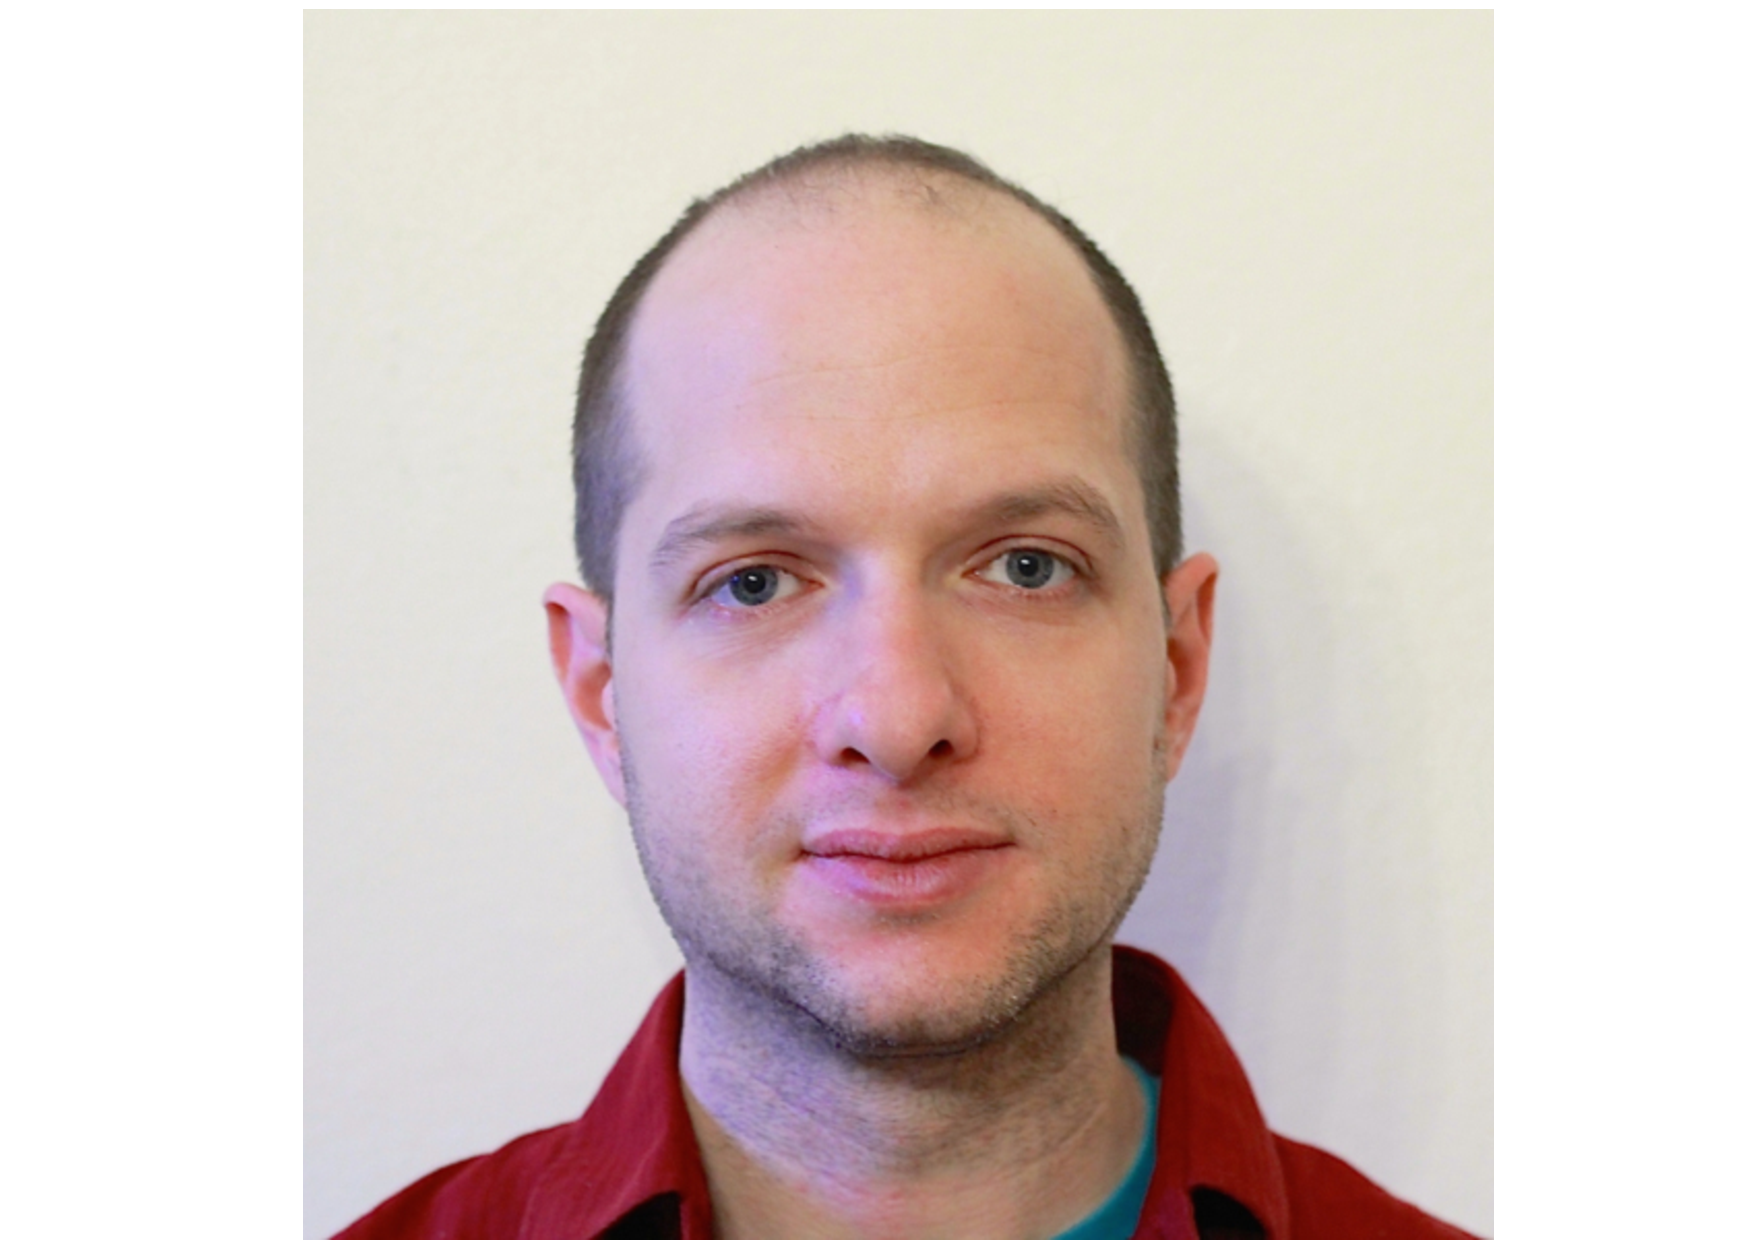
\includegraphics[width=0.3\textwidth]{Mesinger/Author}

Remember to include a brief biography of the Authors or Editors, including a photo.


\chapter*{Contributors}
 
%Only needed for edited collections. Include all contributors, listed alphabetically by surname, along with their affiliation.  


%\raggedright
{\parskip=12pt

\noindent\textbf{Peter Jones}\\
Department of Physics\\
University of New England\\
Acadia, Maine, USA

\noindent\textbf{Simon Smith}\\
Department of Electrical Engineering\\
University of Oxbridge, 
Camford, USA

}

\noindent\textbf{Simon Smith}\\
Department of Electrical Engineering\\
University of Oxbridge, 
Camford, USA

}

\noindent\textbf{Jordan Mirocha}\\
Department of Physics\\
McGill University \\
Montr\'eal, Quebec, Canada
 %only needed for edited books


\mainmatter


%\chapter{Chapter title}

\begin{bf}
  \author{Author Name}\\
  
Abstract\\
\end{bf}

This chapter discusses some important things


\section{A Section}

Lorem ipsum dolor sit amet, consectetur adipiscing elit. Duis eu egestas erat. Maecenas tincidunt lacinia tincidunt. Mauris id lectus nec neque feugiat condimentum vitae at diam. In vel orci nunc, non commodo mauris. Vivamus ipsum enim, vulputate quis pharetra non, molestie quis felis. Vivamus porttitor placerat turpis at accumsan. Nunc tortor velit, faucibus a rhoncus nec, blandit non elit. Nam consectetur lectus eu nisi blandit dapibus rhoncus dui tempus. Mauris fermentum dolor vel ipsum vulputate sit amet ultricies tortor lacinia. Donec ut nibh erat. Morbi nec mi ante. Integer nec vestibulum diam. Donec tincidunt pellentesque quam, ut interdum mauris venenatis condimentum. Nam condimentum, augue in aliquet gravida, neque dui elementum eros, id semper eros purus sed felis. Curabitur in justo sit amet sapien ultrices hendrerit at quis nibh. Quisque iaculis pulvinar tincidunt. 
\begin{eqnarray}
C(12) &= &\left[\overrightarrow{\pi}\cdot\overrightarrow{\phi}(x+r)\right] \nonumber \\ 
&\approx& 1-\mathrm{const}\frac{r^2}{L^2}\int_r^L\frac{x\rmd x}{x^2} + \cdots \nonumber  \\
&\approx& 1-\mathrm{const}\frac{r^2}{L^2}\ln\frac{x\rmd x}{x^2} + \cdots .\label{brokenlongeqn}
\end{eqnarray}

Aenean tellus risus, porta sit amet porta vitae, tincidunt ut felis. Class aptent taciti sociosqu ad litora torquent per conubia nostra, per inceptos himenaeos. Vestibulum ante ipsum primis in faucibus orci luctus et ultrices posuere cubilia Curae; Phasellus pulvinar placerat velit auctor egestas. Vivamus euismod fringilla tincidunt. Sed ut magna felis, id sollicitudin nunc. Quisque a dui eu erat consectetur egestas a quis justo. Aenean euismod congue diam, vel posuere urna fermentum sit amet. Lorem ipsum dolor sit amet, consectetur adipiscing elit. Mauris faucibus lacus eget est mollis auctor. Donec at nibh ligula, et posuere massa. Phasellus quis leo diam \cite{diamantaras1996pcn}.
Donec aliquam blandit risus, eu venenatis ante euismod eu. Curabitur cursus justo id arcu condimentum feugiat. Integer sapien urna, vulputate et adipiscing nec, convallis et justo. Suspendisse in ipsum at felis ornare interdum \cite{tulone2006pts},

\begin{figure}[]
\begin{center}

\includegraphics[width=0.5\textwidth]{Bernardi/01x01-eps-converted-to}
\end{center}
\caption{This is figure 1 in chapter 1.}
\end{figure}

\paragraph{Cras adipiscing} sagittis nunc vel luctus. Suspendisse volutpat augue quis erat semper consequat dignissim tellus euismod. Morbi hendrerit, tellus id aliquam iaculis, nibh leo tincidunt eros, vitae varius ligula felis in mi.

\begin{table}
\caption{Greek Letters.}
\begin{center}
\begin{tabular}{llllllll}
\hline
$\alpha $  & $ \beta $  & $ \gamma $  & $ \delta $  & $ \epsilon $  & $ \varepsilon $  & $ \zeta $  & $ \eta $ \\
 $ \theta $  &  $ \vartheta $  &  $ \gamma $  &  $ \kappa $  &  $ \lambda $  &  $ \mu $  &  $ \nu $  &  $ \xi $ \\
 $ o $  &  $ \pi $  &  $ \varpi $  &  $ \rho $  &  $ \varrho $  &  $ \sigma $  &  $ \varsigma $  &  $$ \\
 $ \tau $  &  $ \upsilon $  &  $ \phi$ &  $ \varphi $  &  $ \chi $  &  $ \psi $  &  $ \omega$  &  $ $ \\
 &  &  &  &  &  &  & \\
$ \Gamma $  & $ \Delta $  & $ \Theta $  &  $ \Lambda $  &  $ \Xi $  &  $ \Pi $  &  $ \Sigma $  & $ \Upsilon $ \\
 $ \Phi$ &  $ \Psi $  &  $ \Omega $  &  &  &  &  &\\
\hline
\end{tabular}
\end{center}\end{table}

\begin{figure}[]
\begin{center}

\includegraphics[width=0.6\textwidth]{Bernardi/01x02}
\end{center}
\caption{This is figure 2 in chapter 1.}
\end{figure}


\bibliographystyle{plain}
\bibliography{Bernardi/References}



\chapter{Theoretical Framework: The Fundamentals of the 21-cm Line}

\begin{bf}
  \author{Steven R. Furlanetto}\\

  Abstract\\

We review some of the fundamental physics necessary for computing the highly-redshifted spin-flip background. We first discuss the radiative transfer of the 21-cm line and define the crucial quantities of interest. We then review the processes that set the spin temperature of the transition, with a particular focus on Wouthuysen-Field coupling, which is likely to be the most important process during and after the Cosmic Dawn. Finally, we discuss processes that heat the intergalactic medium during the Cosmic Dawn, including the scattering of Lyman-$\alpha$, cosmic microwave background, and X-ray photons.
\end{bf}

\section{Radiative Transfer of the 21-cm Line} \label{rt-21cm}

Consider a spectral line labeled by 0 (the lower level) and 1 (the upper level). The radiative transfer equation for the specific intensity $I_\nu$ of photons at the relevant frequency is
\begin{equation}
{dI_\nu\over d\ell}={\phi(\nu) h\nu\over 4\pi}\left[n_1 A_{10} -
\left(n_0 B_{01} -n_1 B_{10}\right)I_\nu\right],
\label{rad}
\end{equation}
where $d\ell$ is a proper path length element, $\phi(\nu)$ is the line profile function, $n_i$
denotes the number density of atoms at the different levels, and $A_{ij}$ and $B_{ij}$ are the Einstein coefficients for the relevant transition (here $i$ and $j$ the initial and final states, respectively). For the 21-cm line, the line frequency is $\nu_{21} = 1420.4057$~MHz. The Einstein relations associate the radiative transition rates via $B_{10}=(g_0/g_1)B_{01}$ and $B_{10}=A_{10}(c^2/2 h\nu^3)$, where $g$ is the spin degeneracy factor of each state. For the 21-cm transition, $A_{10}=2.85\times 10^{-15} \ {\rm s^{-1}}$ and $g_1/g_0=3$.

The relative populations of hydrogen atoms in the two spin states determine the {\bf spin temperature}, $T_S$, through the relation
\begin{equation}
\left({n_1\over n_0}\right)=\left({g_1 \over g_0}\right)
\exp\left\{ {-T_*\over T_S}\right\}, 
\end{equation}
where $T_* \equiv E_{10} /k_B=68$~mK is equivalent to the transition energy $E_{10}$. In almost all physically plausible situations,  $T_\star$ is much smaller than any other temperature, including $T_S$, so all the exponentials in temperature can be Taylor expanded to leading order with high accuracy. Note, however, that $T_S$ implicitly assumes that the level populations can be described by a single temperature -- independent of each atom's velocity. In detail, velocity-dependent effects must be considered in certain circumstances \cite{hirata07}.

It is conventional to replace $I_{\nu}$ by the equivalent {\bf brightness temperature}, $T_b(\nu)$, required of a blackbody radiator (with spectrum $B_{\nu}$) such that $I_{\nu}=B_{\nu}(T_b)$. In the low frequency regime relevant to the 21 cm line, the Rayleigh-Jeans formula is an excellent approximation to the Planck curve, so $T_b(\nu)\approx I_{\nu} \, c^2/2k_B{\nu}^2$.

In this limit, the equation of radiative transfer  along a line of sight through a cloud of uniform excitation temperature $T_S$ becomes
\begin{equation}
T_b'(\nu) = T_{S}(1-e^{-\tau_{\nu}})+T_R'(\nu)e^{-\tau_{\nu}}
\label{eq:rad_trans}
\end{equation}
where $T_b'(\nu)$ is the emergent brightness measured at the cloud and at redshift $z$, the {\bf optical depth}  $\tau_\nu \equiv \int d s \, \alpha_{\nu}$ is the integral of the absorption coefficient ($\alpha_{\nu}$)  along the ray through the cloud, $T_R'$ is the brightness of the background radiation field incident on the cloud along the ray, and $s$ is the proper distance. Because of the cosmological redshift, for the 21-cm transition an observer will measure an apparent brightness at the Earth of $T_b(\nu) = T_b'(\nu_{21})/(1+z)$, where the observed frequency is $\nu=\nu_{21}/(1+z)$. Henceforth we will work in terms of these observed quantities.

The absorption coefficient is related to the Einstein coefficients via
\begin{equation}
\alpha = \phi(\nu) {h \nu \over 4 \pi} (n_0 B_{01} - n_1 B_{10}).
\end{equation}
Because all astrophysical  applications have $T_S \gg T_*$, approximately three of four atoms find themselves in the excited state ($n_0 \approx n_1/3$).  As a result, the stimulated emission correction represented by the first term is significant.  

The fundamental observable quantity is the change in brightness temperature induced by the 21-cm line by a patch of the intergalactic medium (IGM), relative to the incident radiation field. In most models that incident field is simply the cosmic microwave background, although if other sources create a low-frequency radio background at very high redshifts, or if there is a particular source behind the IGM patch along the line of sight from the observer, a larger radio background may exist.

Consider photons incident on the patch from this background. If any redshift into resonance with the 21-cm line, they can interact with the cloud -- but only for a short time, as they will redshift out of resonance as the Universe continues to expand. Thus the Hubble expansion rate sets an effective path length through the cloud, simply equal to the distance the photon travels while it remains within the line profile. The total absorption can be calculated by integrating the IGM density across this interval, in an exactly analogous procedure to the calculation of the Gunn-Peterson Lyman-$\alpha$ optical depth \cite{field59-obs, gunn65, scheuer65}. The result is
\begin{eqnarray}
\tau_{10} & = & \frac{3}{32 \pi} \, \frac{h c^3 A_{10}}{k_B T_S \nu_{10}^2} \, \frac{x_{\rm HI} n_{\rm H}}{(1+z) \, (d v_\parallel/d r_\parallel)}  \label{eq:optdepthcosmo} \\
 & \approx  & 0.0092 \, (1+\delta) \, (1+z)^{3/2}\, \frac{x_{\rm HI}}{T_S} \, \left[ \frac{H(z)/(1+z)}{d v_\parallel/d r_\parallel} \right],
\label{optdepthcosmo-approx}
\end{eqnarray}
where $n_H$ is the hydrogen number density, $x_{\rm HI}$ is the neutral fraction, $dv_\parallel/dr_\parallel$ is the velocity gradient along the line of sight (here scaled to the Hubble flow). In the second part,$T_S$ is in Kelvins, and we have scaled the density to the mean value by writing $n_H = \bar{n}_H^0 (1+z)^3 (1 + \delta)$, where $\bar{n}_H^0$ is the mean comoving density today.

In most circumstances, the CMB provides the background radiation source, for which with temperature $T_\gamma(z)$. Then $T_R' = T_{\gamma}(z)$, so that  we are observing the contrast between high-redshift hydrogen clouds and the CMB.   Because the optical depth is so small, we can then expand the exponentials in equation~(\ref{eq:rad_trans}), and
\begin{eqnarray}
& T_b(\nu) & \approx \frac{T_S-T_{\gamma}(z)}{1+z}\;\tau_{\nu_0} 
\label{eq:dtbone} \\
& \approx & 9\;x_{\rm HI}(1+\delta) \, (1+z)^{1/2}\, \left[1-\frac{T_{\gamma}(z)}{T_S}\right] \, \left[ \frac{H(z)/(1+z)}{d v_\parallel/d r_\parallel} \right] \ \mbox{mK}.
\label{eq:dtb}
\end{eqnarray}
Thus $T_b < 0$ if $T_S < T_{\gamma}$, yielding an absorption signal; otherwise it appears in emission relative to the CMB. Both regimes are likely important for the high-$z$ Universe. Note that $T_b$ saturates if $T_S \gg T_{\gamma}$, but the absorption can become arbitrarily large if $T_S \ll T_{\gamma}$.  The observability of the 21 cm transition therefore hinges on the spin temperature; we will next describe the mechanisms that control that factor.

\section{The Spin Temperature} \label{spin-temp}

Three competing processes determine $T_S$: {\it (i)} absorption of CMB photons (as well as stimulated emission); {\it (ii)} collisions with other particles; and{\it (iii)} scattering of UV photons.  In the presence of the CMB
alone, the spin states reach thermal equilibrium ($T_S=T_{\gamma}$) on a time-scale of $\sim T_*/(T_\gamma A_{10}) = 3 \times 10^5 (1+z)^{-1}$ yr -- much shorter than the age of the Universe at all redshifts after cosmological recombination, indicating that CMB coupling establishes itself rapidly. Indeed all the relevant processes adjust on very short timescales (compared to the Hubble time) so equilibrium is an excellent approximation.

However, the other two processes break this coupling. We let $C_{10}$ and $P_{10}$ be the de-excitation rates (per atom) from collisions and UV scattering, respectively.  We also let $C_{01}$ and $P_{01}$ be the
corresponding excitation rates.  In equilibrium, the spin temperature is then
determined by
\begin{equation}
n_1 \left( C_{10} + P_{10} + A_{10} + B_{10} I_{\rm CMB} \right) = n_0 \left( C_{01} + P_{01} + B_{01} I_{\rm CMB} \right),
\label{eq:detbal}
\end{equation}
where $I_{\rm CMB}$ is the specific intensity of CMB photons at $\nu_{21}$.  With the Rayleigh-Jeans approximation, equation (\ref{eq:detbal}) can be rewritten as
\begin{equation}
T_S^{-1} = \frac{T_\gamma^{-1} + x_c T_K^{-1} + x_\alpha T_c^{-1}}{1 + x_c + x_\alpha},
\label{eq:xdefn}
\end{equation}
where $x_c$ and $x_\alpha$ are coupling coefficients for collisions and UV scattering, respectively, and $T_K$ is the gas kinetic temperature.  Here we have used the principle of detailed balance through the relation
\begin{equation}
\frac{C_{01}}{C_{10}} = \frac{g_1}{g_0} e^{-T_\star/T_K} \approx 3 \left( 1 - \frac{T_\star}{T_K} \right).
\label{eq:c01db}
\end{equation}
We have also \emph{defined} the effective color temperature of the UV radiation field $T_c$ via
\begin{equation}
\frac{P_{01}}{P_{10}} \equiv 3 \left( 1 - \frac{T_\star}{T_c} \right).
\label{eq:tcolor}
\end{equation}
In the limit in which $T_c \rightarrow T_K$ (usually a good approximation), equation~(\ref{eq:xdefn}) may be written 
\begin{equation}
1 - \frac{T_\gamma}{T_S} = \frac{x_c + x_\alpha}{1 + x_c + x_\alpha} \, \left( 1 - \frac{T_\gamma}{T_K} \right).
\label{eq:xdefn-tfac}
\end{equation}

We must now calculate $x_c$,  $x_\alpha$, and $T_c$, which we shall do in the next subsections.

\subsection{Collisional Coupling} \label{coll}

We will first consider collisional excitation and de-excitation of the hyperfine levels, which become important in dense gas.  The coupling coefficient for collisions with species $i$ is
\begin{equation}
x_c^i \equiv  \frac{C_{10}^i}{A_{10}} \, \frac{T_\star}{T_\gamma} = \frac{n_i \, \kappa_{10}^i}{A_{10}} \, \frac{T_\star}{T_\gamma},
\label{eq:xcdefn}
\end{equation}
where $\kappa_{10}^i$ is the rate coefficient for collisional spin de-excitation in collisions (with units of cm$^3$ s$^{-1}$).  The total $x_c$ is the sum over all relevant species $i$, including collisions with (1) neutral hydrogen atoms, (2) free electrons, and (3) protons.  

These rate coefficients can be calculated by the quantum mechanical cross sections of the relevant processes \cite{zygelman05, furl07-electron, furl07-proton}. We will not list them in detail but show the rates in Figure~\ref{fig:collrates}.  Although the atomic cross-section is small, in the unperturbed IGM collisions between neutral hydrogen atoms nearly always dominate these rates because the ionized fraction is small.  Free electrons can be important in partially ionized gas; collisions with protons are only important at the lowest temperatures.

%%%%%: FIGURE: Collision rates
\begin{figure}[]
\begin{center}
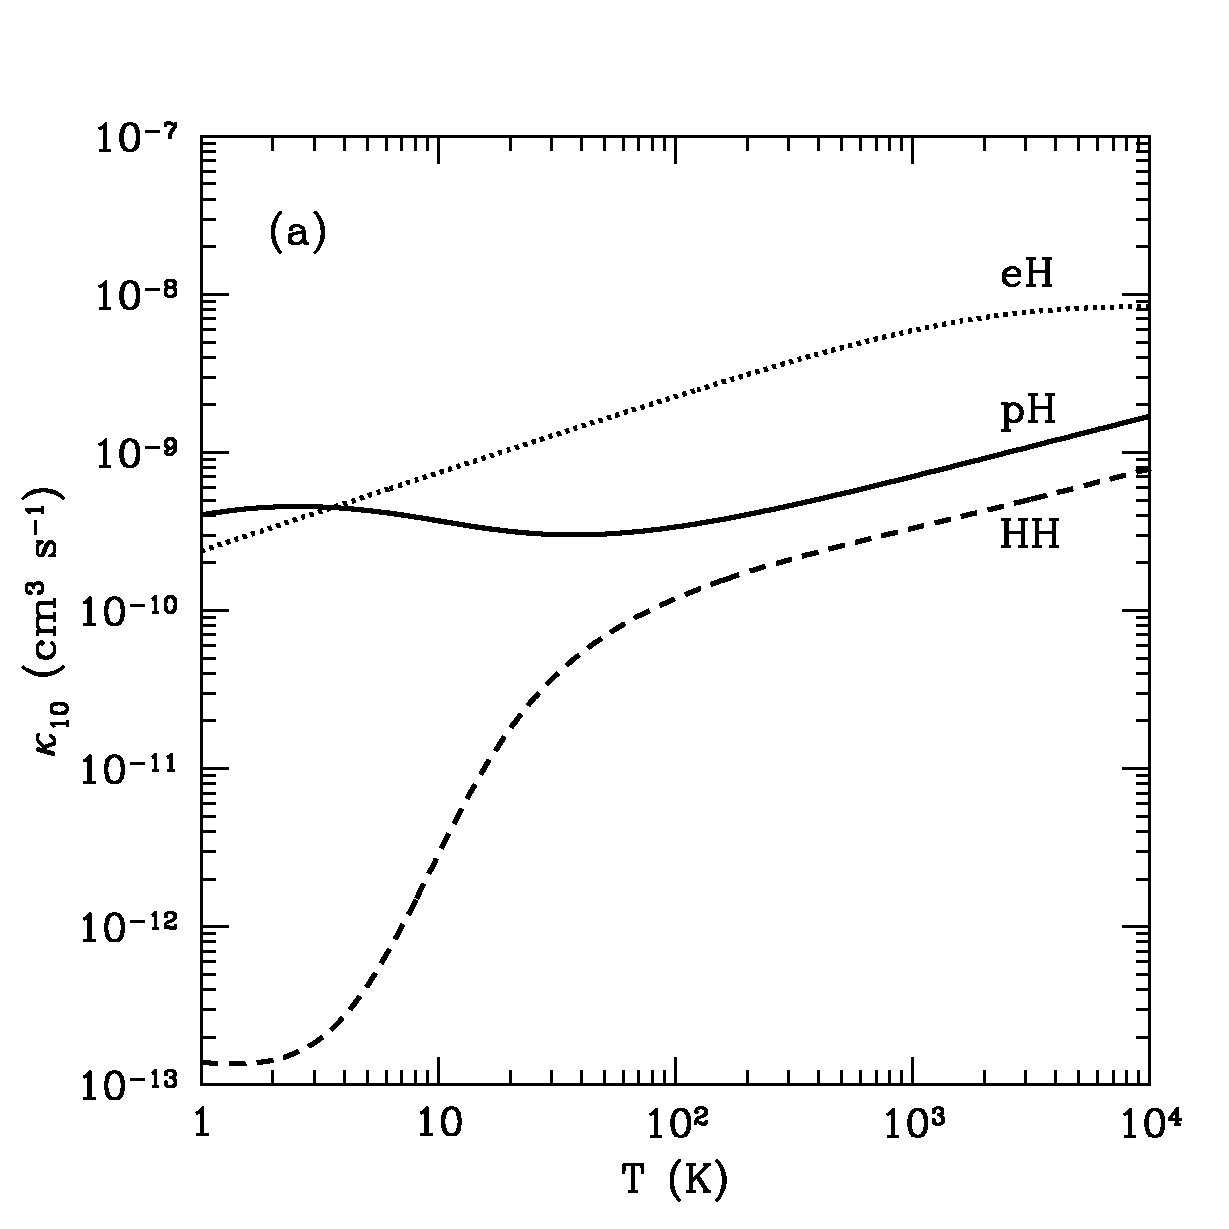
\includegraphics[width=0.5\textwidth]{Furlanetto/figure2-1}
\end{center}
\caption{De-excitation rate coefficients for H-H collisions (dashed
line), H-e$^-$ collisions (dotted line), and H-p collisions (solid
line).  Note that the net rates are also proportional to the densities
of the individual species, so H-H collisions still dominate in a
weakly-ionized medium. From \cite{furl07-proton}.}
\label{fig:collrates}
\end{figure}

Given the densities relevant to the IGM, collisional coupling is quite weak in a nearly neutral, cold medium.  Thus, the local density must be large in order for this process to effectively fix $T_S$. A convenient estimate of their
importance is the critical overdensity, $\delta_{\rm coll}$, at which
$x_c=1$ for H--H collisions:
\begin{equation}
1 + \delta_{\rm coll} = 0.99 \, \left[ \frac{\kappa_{10}(88 \ \mbox{K})}{\kappa_{10}(T_K)} \right] \, \left( \frac{0.023}{\Omega_b
    h^2} \right) \, \left( \frac{70}{1+z} \right)^2,
\label{eq:dcoll}
\end{equation}
where 88~K is the expected IGM temperature at $1+z=70$.\footnote{Note that this is \emph{smaller} than the CMB temperature at this time, because the IGM gas cools faster (due to adiabatic expansion) once Compton scattering becomes inefficient at $z \sim 150$.}  In the standard picture, at redshifts $z < 70$, $x_c \ll 1$ and $T_S \rightarrow T_{\gamma}$; by $z \sim 30$ the IGM essentially becomes invisible.  However, $\kappa_{10}$ is extremely sensitive to $T_K$ in this low-temperature regime.  If the Universe is somehow heated above the fiducial value, the threshold density can remain modest: $\delta_{\rm coll} \approx 1$ at $z=40$ if $T_K=300$~K.

\subsection{The Wouthuysen-Field Effect} \label{wf}

We must therefore appeal to a different mechanism to render the 21-cm transition visible during the era of the first galaxies.  This is known as the {\bf Wouthuysen-Field mechanism} (named after the Dutch physicist Siegfried
Wouthuysen and Harvard astrophysicist George Field who first explored it \cite{wouthuysen52, field58}). Figure~\ref{fig:wf} illustrates the effect. This shows the hyperfine sub-levels of the $1S$ and $2P$ states of HI and the permitted transitions between them.  Suppose a hydrogen atom in the hyperfine singlet state absorbs a Lyman-$\alpha$ photon.  The electric dipole selection rules allow $\Delta F=0,1$ except that $F=0 \rightarrow 0$ is prohibited (here $F$ is the total angular momentum of the atom).  Thus the atom must jump to either of the central $2P$ states.  However, these same rules now allow electrons in either of these excited states to decay to the $_1S_{1/2}$ triplet level.\footnote{Here we use the notation $_F L_J$, where $L$ and $J$ are the orbital and total angular momentum of the electron.}  Thus, atoms can change hyperfine states through the absorption and spontaneous re-emission of a Lyman-$\alpha$ photon (or indeed any Lyman-series photon; see below).

%%%%%: FIGURE: W-F levels
\begin{figure}[]
\begin{center}
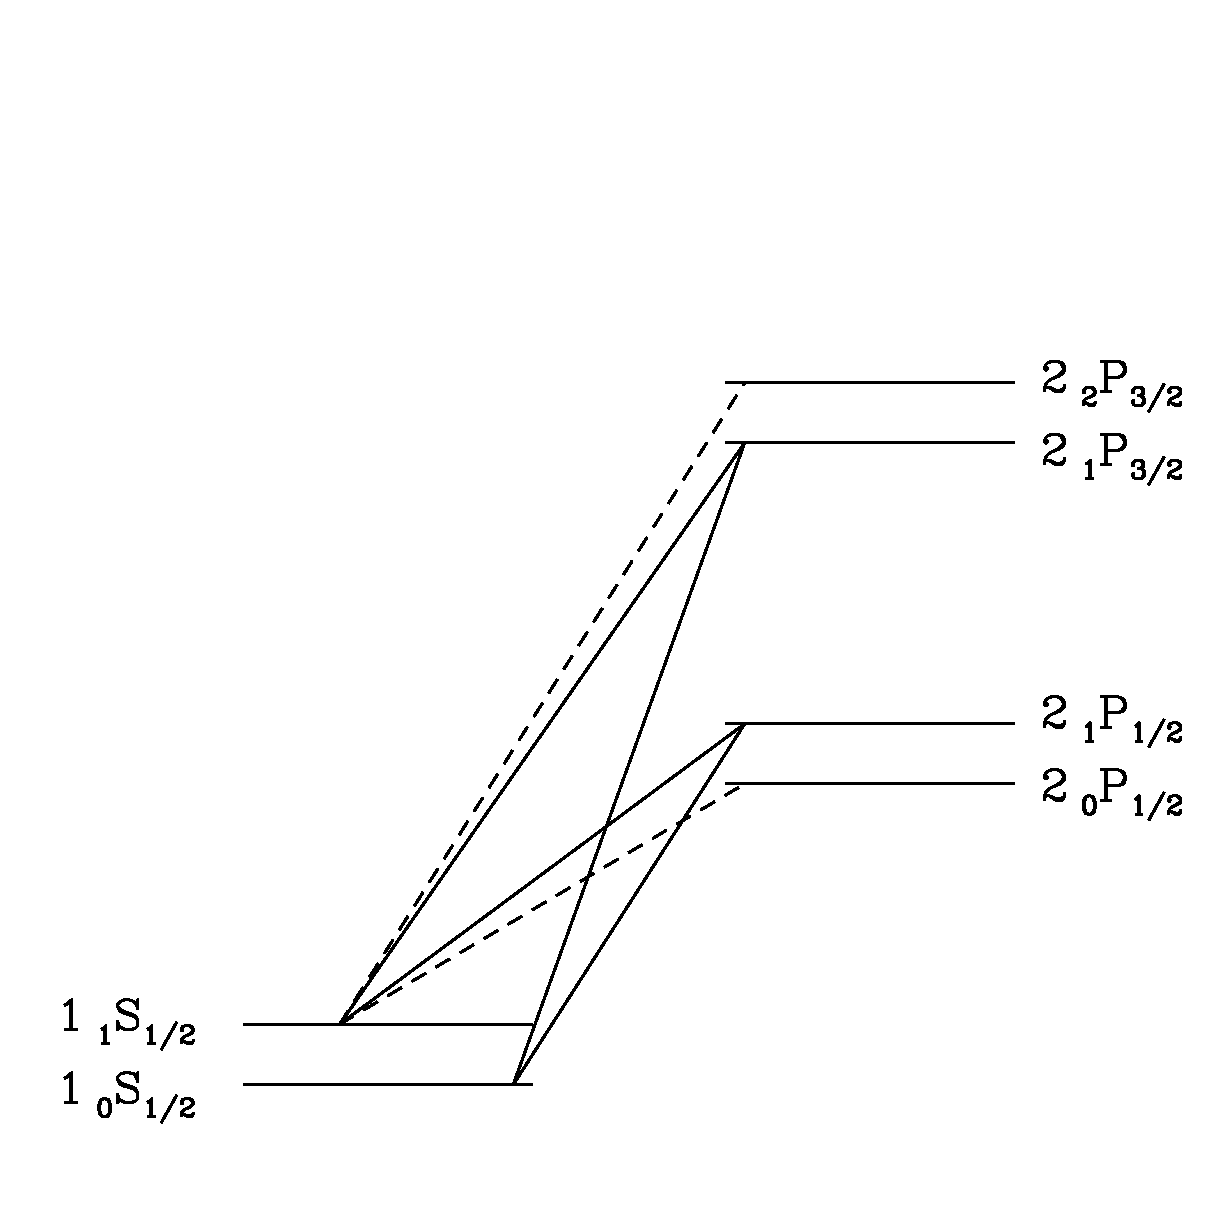
\includegraphics[width=0.6\textwidth]{Furlanetto/figure2-2}
\end{center}
\caption{Level diagram illustrating the Wouthuysen-Field effect.  We show the hyperfine splittings of the $1S$ and $2P$ levels.  The solid lines label transitions that can mix the ground state hyperfine levels, while the dashed lines label complementary allowed transitions that do not participate in mixing.  From \cite{pritchard06}.}
\label{fig:wf}
\end{figure}

The Wouthuysen-Field coupling rate depends ultimately on the total rate (per atom) at which Lyman-$\alpha$ photons scattered through the gas,
\begin{equation}
P_\alpha = 4 \pi \sigma_0 \int d \nu \, J_\nu(\nu) \phi_\alpha(\nu),
\label{eq:palpha}
\end{equation}
where $\sigma_\nu \equiv \sigma_0 \phi_\alpha(\nu)$ is the local Lyman-$\alpha$ absorption cross section, $\sigma_0 \equiv (\pi \, e^2/m_e \, c) f_{\alpha}$, $f_\alpha=0.4162$ is the oscillator strength of the Lyman-$\alpha$ transition, $\phi_\alpha(\nu)$ is the Lyman-$\alpha$ absorption profile, and $J_\nu$ is the angle-averaged specific intensity of the background radiation field.\footnote{By convention, we use the specific intensity in units of photons cm$^{-2}$ Hz$^{-1}$ s$^{-1}$ sr$^{-1}$ here, which is conserved during the expansion of the Universe (whereas a definition in terms of energy instead of photon number is subject to redshifting).}   

Transitions to higher Lyman-$n$ levels have similar effects \cite{hirata06, pritchard06}. Suppose that a UV photon redshifts into the Lyman-$n$ resonance as it travels through the IGM.  After absorption, it can either scatter (by the electron decaying directly to the ground state) or cascade through a series of intermediate levels and produce a sequence of photons.  The direct decay probability for any level is $\sim 0.8$, so a Lyman-$n$ photon will typically scatter $N_{\rm scatt} \approx (1-P_{nP\rightarrow1S})^{-1} \sim 5$ times before instead initiating a decay cascade.  In contrast, Lyman-$\alpha$ photons scatter hundreds of thousands of times before being destroyed, usually be redshifting all the way across the (very wide) Lyman-$\alpha$ profile.  As a result, coupling from the direct scattering of Lyman-$n$ photons is suppressed compared to Lyman-$\alpha$ by a large factor.

However, Lyman-$n$ photons can still be important because of their cascade products, as shown in Figure~\ref{fig:lygamma}.  Following Lyman-$\beta$ absorption, the only permitted decays are to the ground state (regenerating a Lyman-$\beta$ photon and starting the process again) or to the $2S$ level.  The H$\alpha$ photon produced in the $3P \rightarrow 2S$ transition (and indeed any photon produced in a decay to an excited state) escapes to infinity. Thus the atom will eventually find itself in the $2S$ state, which decays to the ground state via a forbidden two photon process with $A_{2S\rightarrow1S}=8.2$~s$^{-1}$.  These photons will also escape to infinity, so coupling from Lyman-$\beta$ photons can be completely neglected.\footnote{In a medium with very high number density, atomic collisions can mix the two angular momentum states, but that process is unimportant in the IGM.}

But now consider excitation by Lyman-$\gamma$, also shown in Figure~\ref{fig:lygamma}.  This can cascade (through $3S$ or $3D$) to the $2P$ level, in which case the original Lyman-$n$ photon is ``recycled'' into a Lyman-$\alpha$ photon, which then scatters many times through the IGM.  Thus, the key quantity for determining the coupling induced by Lyman-$n$ photons is the fraction $f_{\rm rec}(n)$ of cascades that terminate in Lyman-$\alpha$ photons.  Our discussion in the previous paragraph shows that $f_{\rm rec}(n=3)$ vanishes, but detailed quantum mechanical calculations show that the higher states all have $f_{\rm rec} \sim 1/3$ \cite{hirata06, pritchard06}. 

Focusing again on the Lyman-$\alpha$ photons themselves, we must relate the total scattering rate $P_\alpha$ to the indirect de-excitation rate $P_{10}$ \cite{field58, meiksin00}. Let us first label the $1S$ and $2P$ hyperfine levels a--f, in order of increasing energy, and let $A_{ij}$ and $B_{ij}$ be the spontaneous emission and absorption coefficients for transitions between these levels.  We write the background intensity at the frequency corresponding to the $i \rightarrow j$ transition as $J_{ij}$.  Then
\begin{equation}
P_{01} \propto B_{\rm ad} J_{\rm ad} \frac{A_{\rm db}}{A_{\rm da} + A_{\rm db}} + B_{\rm ae} J_{\rm ae} \frac{A_{\rm eb}}{A_{\rm ea} + A_{\rm eb}}.\label{eq:psum}
\end{equation}
The first term contains the probability for an a$\rightarrow$d transition ($B_{\rm ad} J_{\rm ad}$), together with the probability for the subsequent decay to terminate in state b; the second term is the same for transitions to and from state e (see Figure~\ref{fig:wf}).  Next we need to relate each$A_{ij}$ to the total spontaneous decay rate from the $2P$ level, $A_\alpha = 6.25 \times 10^8$~Hz, the total Lyman-$\alpha$ spontaneous emission rate.  This can be accomplished using a sum rule stating that the sum of decay intensities ($g_i A_{ij}$) for transitions from a
given $nFJ$ to all the $n' J'$ levels (summed over $F'$) is proportional to $2F+1$, which implies that the relative strengths of the permitted transitions are then $(1,\,1,\,2,\,2,\,1,\,5)$, where we have ordered the lines by (initial, final) states (bc, ad, bd, ae, be, bf).  With our assumption that the background radiation field is constant across the individual hyperfine lines, we find $P_{10} = (4/27) P_\alpha$ \cite{meiksin00}.

The coupling coefficient $x_\alpha$ is then
\begin{equation}
x_\alpha = \frac{4 P_\alpha}{27 A_{10}} \, \frac{T_\star}{T_{\gamma}} \equiv S_\alpha \frac{J_\alpha}{J_\nu^c}.
\label{eq:xalpha}
\end{equation}
The second part evaluates $J_\nu$ ``near" line center and sets $J_\nu^c \equiv 1.165 \times 10^{-10} [(1+z)/20]$~photons cm$^{-2}$ sr$^{-1}$ Hz$^{-1}$ s$^{-1}$.   $S_\alpha$ s a correction factor that accounts for (complicated) radiative transfer effects in the intensity near the line center (see below).  The coupling threshold $J_\nu^c$ for $x_\alpha = S_\alpha$ can also be written in terms of the number of Lyman-$\alpha$ photons per hydrogen atom in the Universe, which we denote $\tilde{J}_\nu^c = 0.0767 \, [(1+z)/20]^{-2}$.  This threshold is relatively easy to achieve in practice.

To complete the coupling calculation, we must determine $T_c$ and the correction factor $S_\alpha$.  The former is the effective temperature of the UV radiation field, defined in equation~(\ref{eq:tcolor}), and is determined by the shape of the photon spectrum at the Lyman-$\alpha$ resonance. The effective temperature of the radiation field \emph{must} matter, because the energy deficit between the different hyperfine splittings of the Lyman-$\alpha$ transition (labeled bc, ad, etc. above) implies that the mixing process is sensitive to the gradient of the radiation spectrum near the Lyman-$\alpha$ resonance.  More precisely, the procedure described after equation~(\ref{eq:psum}) yields
\begin{equation}
\frac{P_{01}}{P_{10}} = \frac{g_1}{g_0} \, \frac{n_{\rm ad} + n_{\rm ae}}{n_{\rm bd} + n_{\rm be}} \approx 3 \left( 1 + \nu_0 \frac{d \ln n_\nu}{d \nu} \right),
\label{eq:tcrad1}
\end{equation}
where $n_\nu = c^2 \, J_\nu/2 \nu^2$ is the photon occupation number.
Thus, by comparison to equation~(\ref{eq:tcolor}) we find
\begin{equation}
\frac{h}{k_B T_c} = - \frac{d \ln n_\nu}{d \nu}.
\label{eq:tcrad}
\end{equation}

A simple argument shows that $T_c \approx T_K$ \cite{field59-ts}: so long as the medium is extremely optically thick, the enormous number of Lyman-$\alpha$ scatterings forces the Lyman-$\alpha$ profile to be a blackbody of temperature $T_K$ near the line center.  This condition is easily fulfilled in the high-redshift IGM, where $\tau_\alpha \gg 1$.  In detail, atomic recoils during scattering tilt the spectrum to the red and are primarily responsible for establishing this equilibrium \cite{field59-res}.  

%%%%%: FIGURE: Radiative cascades
\begin{figure}[]
\begin{center}
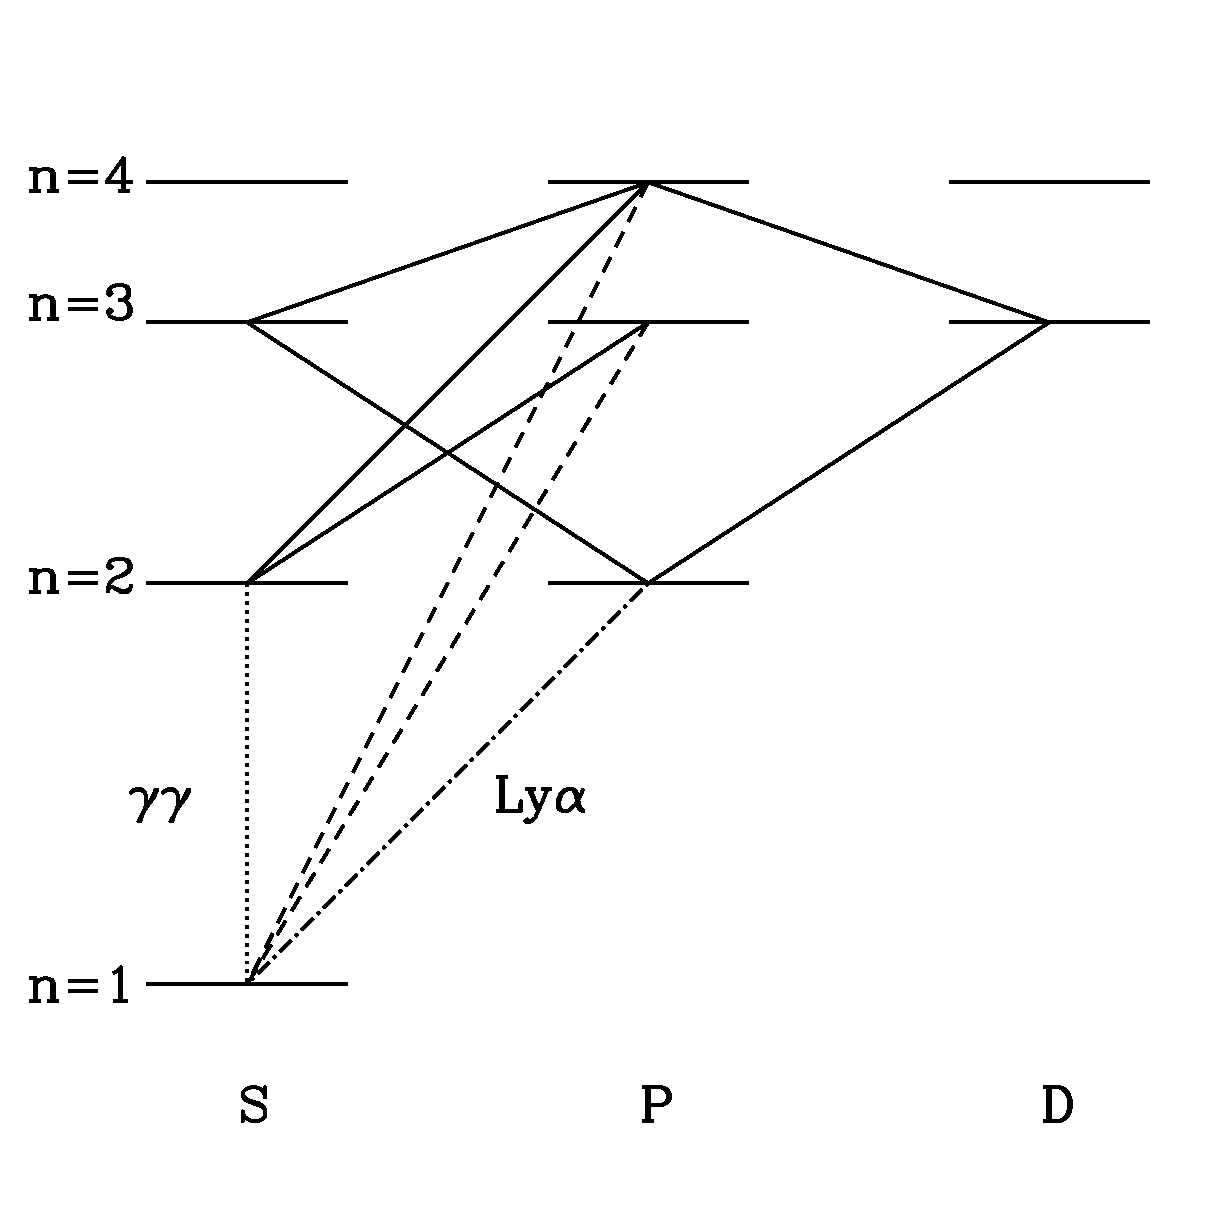
\includegraphics[width=0.6\textwidth]{Furlanetto/figure2-3}
\end{center}
\caption{Decay chains for Lyman-$\beta$ and Lyman-$\gamma$ excitations.  We show
  Lyman-$n$ transitions by dashed curves, Lyman-$\alpha$ by the dot-dashed
  curve, cascades by solid curves, and the forbidden $2S \rightarrow
  1S$ transition by the dotted curve. From \cite{pritchard06}.}
\label{fig:lygamma}
\end{figure}

The physics of the Wouthuysen-Field effect are actually much more complicated than naively expected because scattering itself modifies the shape of $J_\nu$ near the Lyman-$\alpha$ resonance \cite{chen04}. In essence, the spectrum must develop an absorption feature because of the increased scattering rate near the Lyman-$\alpha$ resonance. Photons lose energy at a fixed rate by redshifting, but each time they scatter they also lose a small amount of energy through recoil.  Momentum conservation during each scattering slightly decreases the frequency of the photon.  The strongly enhanced scattering rate near line center means that photons ``flow" through
that region more rapidly than elsewhere (where only the cosmological redshift applies), so the amplitude of the spectrum must be smaller.  Meanwhile, the scattering in such an optically thick medium also causes photons to diffuse away from line center, broadening the feature well beyond the nominal line width.

If the fractional frequency drift rate is denoted by ${\mathcal A}$, continuity requires $n_\nu {\mathcal A}=$~constant. Because ${\mathcal A}$ increases near resonance, the number density must fall.  On average, the energy loss (or gain) per scattering is \cite{chen04}
\begin{equation}
\frac{\Delta E_{\rm recoil}}{E} = \frac{h \nu}{m_p c^2} \, \left(1 - \frac{T_K}{T_c} \right),
\label{eq:recoil-loss}
\end{equation}
where the first factor comes from recoil off an isolated atom and the second factor corrects for the distribution of initial photon energies; the energy loss vanishes when $T_c = T_K$, and when $T_c < T_K$, the gas is heated by the scattering process.

To compute $S_\alpha$, we must calculate the photon spectrum near Lyman-$\alpha$.  We begin with the radiative
transfer equation in an expanding universe (written in comoving coordinates, and again using units of ~photons cm$^{-2}$ sr$^{-1}$ Hz$^{-1}$ s$^{-1}$ for $J_\nu$:
\begin{equation}
\frac{1}{c n_H \sigma_0} \, \frac{\partial J_\nu}{\partial t} = -\phi_\alpha(\nu) \, J_\nu + H \nu_\alpha \, \frac{\partial J_\nu}{\partial \nu} + \int d \nu' \, R(\nu,\nu') \, J_{\nu'} + C(t) \psi(\nu).
\label{eq:rt21}
\end{equation}
The first term on the right-hand side describes absorption, the second describes redshifting due to the Hubble flow, and the third accounts for re-emission following absorption.  $R(\nu,\nu')$ is the ``redistribution function" that specifies the frequency of an emitted photon, which depends on the relative momenta of the absorbed and
emitted photons as well as the absorbing atom. The last term accounts for the injection of new photons (via, e.g., radiative cascades that result in Lyman-$\alpha$ photons): $C$ is the rate at which they are produced and $\psi(\nu)$ is their frequency distribution.

The redistribution function $R$ is the difficult aspect of the problem, but it can be simplified if the frequency change per scattering (typically of order the absorption line width) is ``small."  In that case, we can expand $J_{\nu'}$ to second order in $(\nu-\nu')$ and rewrite equation~(\ref{eq:rt21}) as a diffusion problem in frequency.
The steady-state version of equation (\ref{eq:rt21}) becomes, in this so-called {\it Fokker-Planck} approximation, \cite{chen04}
\begin{equation}
\frac{d}{d x} \left( - {\mathcal A} \, J + {\mathcal D} \, \frac{d J}{d x} \right) + C \psi(x) = 0,
\label{eq:fokker}
\end{equation}
where $x \equiv (\nu-\nu_\alpha)/\Delta \nu_D$, $\Delta \nu_D$ is the Doppler width of the absorption profile, ${\mathcal A}$ is the frequency drift rate, and ${\mathcal D}$ is the diffusivity.  The Fokker-Planck approximation is valid so long as (i) the frequency change per scattering ($\sim \Delta \nu_D$) is smaller than the width of any spectral features, and either (iia) the photons are outside the line core where the Lyman-$\alpha$ line profile is slowly changing, or (iib) the atoms are in equilibrium with $T_c \approx T_K$.

Solving for the spectrum including scattering thus reduces to specifying ${\mathcal A}$ and ${\mathcal D}$.  The drift involves the Hubble flow, which sets ${\mathcal A}_H= - \tau_\alpha^{-1}$, where $\tau_\alpha$ is the Gunn-Peterson optical depth for the Lyman-$\alpha$ line \cite{gunn65, scheuer65}:
\begin{equation}
\tau_{\alpha} = \frac{\chi_\alpha \, n_{\rm HI}(z) \, c}{H(z) \nu_\alpha} \approx 3 \times 10^5 \, x_{\rm HI} \, \left( \frac{1+z}{7} \right)^{3/2}.
\label{eq:taugp}
\end{equation}
Because it is uniform, the Hubble flow does not introduce any diffusion. The remaining terms come from $R$ and
incorporate all the physical processes relevant to energy exchange in scattering.  The drift from recoil causes \cite{hirata06}
\begin{eqnarray}
{\mathcal D}_{\rm scatt} & = & \phi_\alpha(x)/2,
\label{eq:Dkin} \\
{\mathcal A}_{\rm scatt} & = &  -(\eta - x_0^{-1} ) \phi_\alpha(x),
\label{eq:Akin}
\end{eqnarray}
where $x_0 \equiv \nu_\alpha/\Delta \nu_D$ and $\eta \equiv (h \nu_\alpha^2)/(m_p c^2 \Delta \nu_D)$.  The latter is the recoil parameter measuring the average loss per scattering in units of the Doppler width.  The small energy defect between the hyperfine levels provides another source of slow energy exchange \cite{hirata06} and can be incorporated into the scattering in nearly the same way as recoil.

We can now solve equation~(\ref{eq:fokker}) once we choose the boundary conditions, which essentially correspond to the input photon spectrum (ignoring scattering) and the source function.  Because the
frequency range of interest is so narrow, two cases suffice: a flat input spectrum (which approximately describes photons that redshift through the Lyman-$\alpha$ resonance, regardless of the initial source spectrum)
and a step function, where photons are ``injected" at line center (through cascades or recombinations) and redshift away.  In either case, the first integral over $x$ in equation~(\ref{eq:fokker}) is trivial. At high temperatures where spin flips are unimportant to the overall energy exchange, we can write
\begin{equation}
\phi \frac{d J}{d x} + 2 \{ [\eta - (x + x_0)^{-1}] \phi + \tau_\alpha^{-1} \} J = 2 K / \tau_\alpha.
\label{eq:fokk-simp}
\end{equation}
The integration constant $K$ equals $J_\infty$, the flux far from resonance, both for photons that redshift into the line and for injected photons at $x<0$ (i.e., redward of line center); it is zero for injected photons at $x>0$.  

The formal analytic solution, when $K \neq 0$, is most compactly written in terms of $\delta_J \equiv (J_\infty -
J)/J_\infty$ \cite{chen04}:\footnote{Here we assume the gas has a sufficiently high temperature that the different hyperfine sub-transitions can be treated as one \cite{hirata06}.}
\begin{equation}
\delta_J(x) = 2 \eta \int_0^\infty d y \exp \left[ - 2 \{ \eta - (x+x_0)^{-1}\} y - {2 \over \tau_\alpha} \int_{x-y}^{x} \frac{d x'}{\phi_\alpha(x')} \right].
\label{eq:dj-soln}
\end{equation}
(An analogous form also exists for photons injected at line center.) The full problem, including the intrinsic Voigt profile of the Lyman-$\alpha$ line, must be solved numerically, but including only the Lorentzian wings from natural broadening allows a simpler solution \cite{furl06-lyheat}.  Fortunately, this assumption is quite accurate in the most interesting regime of  $T_K <  1000$~K.

%%%%%: FIGURE: Lyman-alpha spectral shape
\begin{figure}[]
\begin{center}
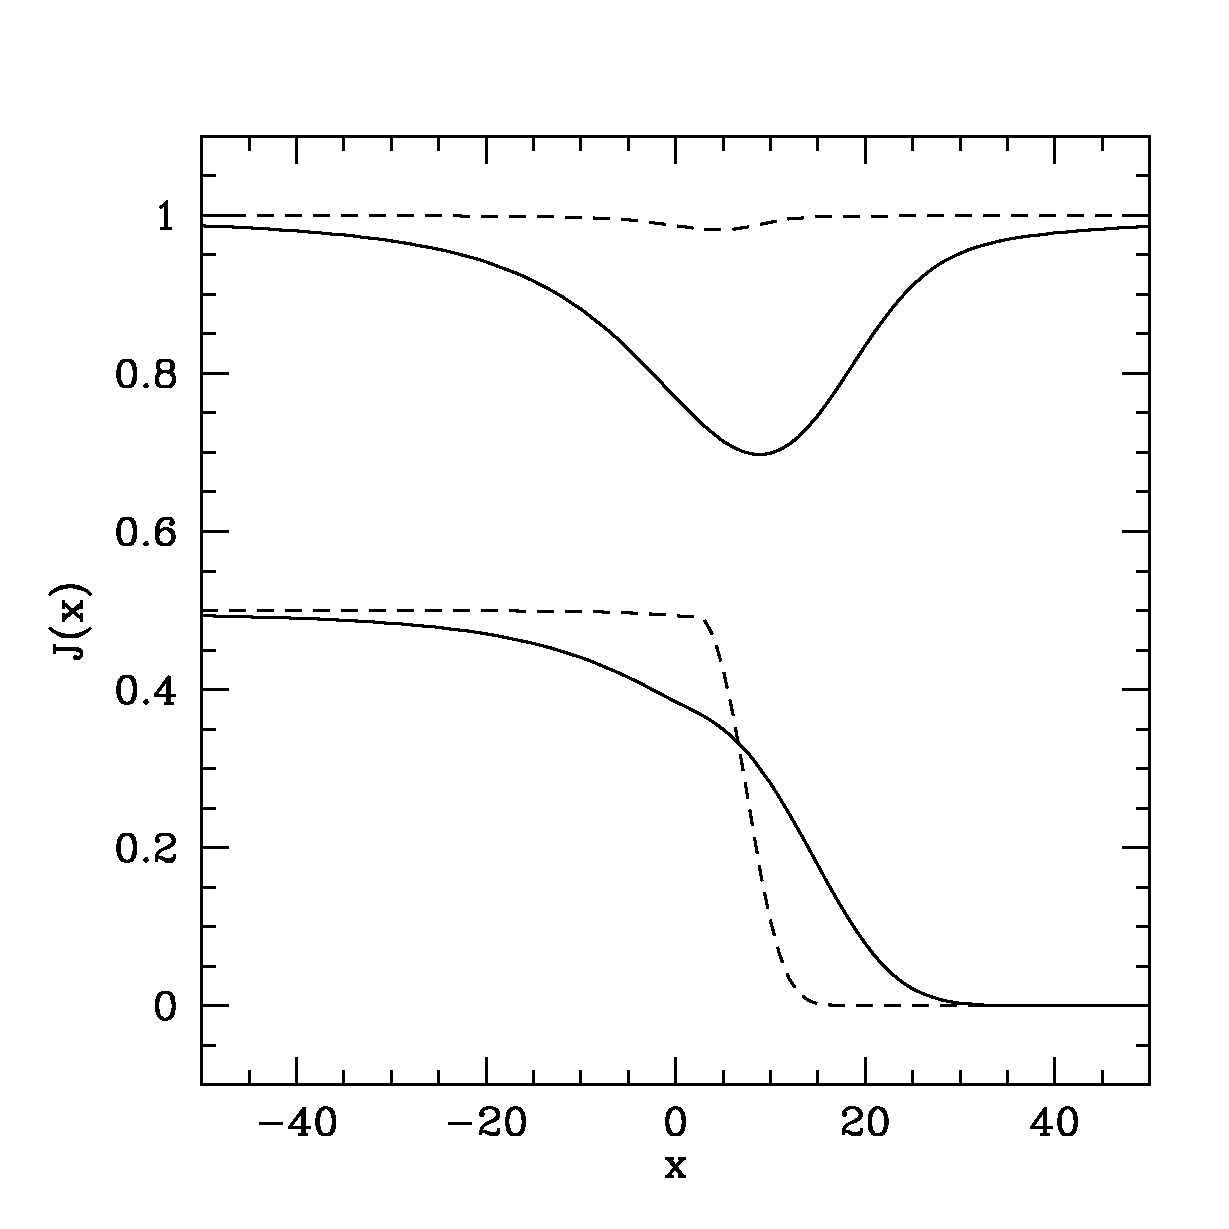
\includegraphics[width=0.6\textwidth]{Furlanetto/figure2-4}
\end{center}
\caption{Background radiation field near the Lyman-$\alpha$ resonance at $z=10$;
$x \equiv (\nu-\nu_\alpha)/\Delta \nu_D$ is the normalized deviation
from line center, in units of the Doppler width.  The upper and lower sets are for continuous photons
and photons injected at line center, respectively.  (The former are
normalized to $J_\infty$; the latter have arbitrary normalization.)
The solid and dashed curves take $T_K=10$ and $1000$~K,
respectively.  From \cite{furl06-lyheat}.}
\label{fig:lyshape}
\end{figure}

The crucial aspect of equation~(\ref{eq:dj-soln}) is that (as expected from the qualitative argument) an absorption feature appears near the line center, with its depth roughly proportional to $\eta$, our recoil parameter.  The feature is more significant when $T_K$ is small (because in that case the average effect of recoil is large). Figure~\ref{fig:lyshape} shows some example spectra (both for a continuous background and for photons injected at line center).

Usually, the most important consequence is the suppression of the radiation spectrum at line center compared to the assumed initial condition.  This decreases the total scattering rate of Lyman-$\alpha$ photons (and hence the Wouthuysen-Field coupling), with the suppression factor (defined in equation~\ref{eq:xalpha}) as \cite{chen04} 
\begin{equation}
S_\alpha = \int_{-\infty}^\infty d x \, \phi_\alpha(x)\, J(x) \approx
[1 - \delta_J(0)] \le 1,
\label{eq:salpha-defn}
\end{equation}
where the second equality follows from the narrowness of the line profile.  Again, the Lorentzian wing approximation turns out to be an excellent one; when $T_K \gg T_\star$, the suppression is \cite{furl06-lyheat}
\begin{equation} S_\alpha \sim \exp \left[ -0.803 \left({T_K\over
1~{\rm K}}\right)^{-2/3} \left( \frac{\tau_\alpha}{10^{6}}
\right)^{1/3} \right].
\label{eq:salpha-approx}
\end{equation}
Note that this form applies to both photons injected at line center as well as those that redshift in from infinity.  As we can see in Figure~\ref{fig:lyshape}, the suppression is most significant in cool gas.


\section{Heating of the Intergalactic Medium} 

We have seen that both collisions and the Wouthuysen-Field effect couple the spin temperature to the kinetic temperature of the gas. The 21-cm brightness temperature therefore depends on processes that heat the IGM. We will review several such mechanisms in this section.

\subsection{The Lyman-$\alpha$ Background}

The photons that trigger Lyman-$\alpha$ coupling exchange energy with the IGM, through the recoil in each scattering event. The typical energy exchange per scattering is small (see eq. \ref{eq:recoil-loss}), but the scattering rate is extremely large.  If the net heating rate per atom followed the naive expectation, $\sim
P_\alpha \times (h \nu_\alpha)^2/m_p c^2$, the kinetic temperature would surpass $T_\gamma$ soon after Wouthuysen-Field coupling becomes efficient.

However, the details of radiative transfer radically change these expectations \cite{chen04}.  In a static medium, the energy exchange \emph{must} vanish in equilibrium even though scattering continues at nearly the same rate.
Scattering induces an asymmetric absorption feature near $\nu_\alpha$ (Figure~\ref{fig:lyshape}) whose shape depends on the combined effects of atomic recoils and the scattering diffusivity.  In equilibrium, the latter exactly counterbalances the former.  

If we removed scattering, the absorption feature would redshift away as the Universe expands. Thus, the energy exchange rate from scattering must simply be that required to maintain the feature in place.  For photons redshifting into resonance, the absorption trough has total energy 
\begin{equation}
\Delta u_\alpha = (4\pi/c) \int (J_\infty - J_\nu) h \nu d \nu,
\end{equation}
where $J_\infty$ is the input spectrum, and we note that the $h \nu$ factor converts from our definition of specific intensity (which counts photons) to energy.  The radiation background loses $\epsilon_\alpha = H \Delta u_\alpha$ per
unit time through redshifting; this energy goes into heating the gas.
Relative to adiabatic cooling by the Hubble expansion, the fractional
heating amplitude is
\begin{eqnarray}
\frac{2}{3} \, \frac{\epsilon_\alpha}{k_B T_K n_H H(z) } & = & \frac{8 \pi}{3} \, \frac{h \nu_\alpha}{k_B T_K} \, \frac{J_\infty \, \Delta \nu_D}{c n_H} \, \int_{-\infty}^{\infty} d x \delta_J(x) \label{eq:epsalpha}
\\
& \approx & \frac{0.80}{T_K^{4/3}} \, \frac{x_\alpha}{S_\alpha} \left( \frac{10}{1+z} \right),
\label{eq:lyaheat}
\end{eqnarray}
Here we have evaluated the integral for the continuum photons that
redshift into the Lyman-$\alpha$ resonance; the ``injected" photons
actually cool the gas slightly.  The net energy exchange when
Wouthuysen-Field coupling becomes important (at $x_\alpha \sim
S_\alpha$) is therefore just a fraction of a degree, and in practice gas heating through Lyman-$\alpha$ scattering
is generally unimportant \cite{chen04,furl06-lyheat}.

Fundamentally, Lyman-$\alpha$ heating is inefficient because scattering diffusivity cancels the effects of recoil.  From Figure~\ref{fig:lyshape}, we see that the background spectrum is weaker on the blue side of the line than on the red.  The scattering process tends to move the photon toward line center, with the extra energy deposited in or extracted from the gas.  Because more scattering occurs on the red side, this tends to transfer energy from the gas back to the photons, mostly canceling the energy obtained through recoil.

\subsection{The Cosmic Microwave Background} 

The previous section shows that, when considered as a two-level process that acts in isolation, Lyman-$\alpha$ scattering has only a slight effect on the gas temperature. However, in reality this Lyman-$\alpha$ scattering always occurs in conjunction with scattering of CMB photons within the 21-cm transition. The combination leads to an enhanced heating rate \cite{venumadhav18}.

In essence, the process works as follows. The CMB photons scatter through the hyperfine levels of HI to heat those atoms above their expected temperature (determined in this simple case by adiabatic cooling). Meanwhile, Lyman-$\alpha$ photons scatter through the gas as well. As they do so, they mix the hyperfine levels of the HI ground state, as depicted in Figure~\ref{fig:wf} -- this is the Wouthuysen-Field effect. CMB scattering continues to heat the hyperfine level populations during the Lyman-$\alpha$ scattering, which then sweeps up this extra energy and ultimately deposits it as thermal energy through the net recoil effect.

We can estimate the energy available to this heating mechanism by considering the CMB energy reservoir \cite{venumadhav18}. The CMB energy density at the 21-cm transition is $u_\nu = (4 \pi/c) B_\nu \approx 8 \pi (\nu_{21}^2/c^3) k_B T_\gamma$. Over a redshift interval $\Delta z=1$, the total energy that redshifts through the line is $u_\nu \Delta \nu \approx 8 \pi (\nu_{21}/c)^3 k_B T_\gamma / (1+z)^2$. However, only a fraction $\tau_{10}$ actually interacts with the line. If all of this energy is used for heating, the temperature change per H atom would be
\begin{equation}
\Delta T_{\rm CMB-Ly\alpha} \approx \tau_{10} {u_\nu \Delta_\nu \over (3/2) n_H} \approx 5 x_{\rm HI} \  \left( {1 + z \over 20} \right)^{-1/2} \left( {10 \ {\rm K} \over T_S} \right) \ {\rm K}.
\label{eq:cmb-lya-heat}
\end{equation}

A more detailed calculation of the heating rate shows that it is somewhat slower, but it does amplify the effect of the Lyman-$\alpha$ heating alone by a factor of several \cite{venumadhav18}. In standard models of the early radiation backgrounds, the correction is still relatively modest, but it is not negligible. For example, in the fiducial model considered by \cite{venumadhav18}, the Lyman-$\alpha$ heating on its own modifies $T_K$ by $\sim 1$--5\%, but with the CMB scattering included the effect is $\sim 9$--15\%. Additionally, the CMB scattering can be enhanced in some exotic physics models that decrease the spin temperature substantially.

\subsection{The X-ray Background} 

Because they have relatively long mean free paths, X-rays from galaxies and quasars are likely to be the most important heating agent for the low-density IGM  \cite{madau97}.  In particular, photons with $E>1.5 x_{\rm HI}^{1/3} [(1+z)/10]^{1/2}$~keV have mean free paths exceeding the Hubble length \cite{oh01}.  Lower-energy X-rays will be absorbed in the IGM, depositing much of their energy as heat, as will a fraction of higher-energy X-rays.

X-rays heat the IGM gas by first photoionizing a hydrogen or helium atom.  The resulting ``primary'' electron retains most of the photon energy (aside from that required to ionize it) as kinetic energy, which it must then distribute to the general IGM through three main channels: (1) collisional ionizations, which produce more secondary electrons that themselves scatter through the IGM, (2) collisional excitations of HeI (which produce photons capable of ionizing HI) and HI (which produces a Lyman-$\alpha$ background), and (3) Coulomb collisions with free electrons (which distributes the kinetic energy .  The relative cross-sections of these processes determines what fraction of the X-ray energy goes to heating ($f_{\rm heat}$), ionization ($f_{\rm ion}$), and excitation ($f_{\rm excite}$); clearly it depends on both the ionized fraction $x_i$ and the input photon energy.  Through these scatterings, the primary photoelectrons, with $T \sim 10^6$~K, rapidly cool to energies just below the Lyman-$\alpha$ threshold, $<10$~eV, and thus equilibrate with the other IGM electrons.  After that, the electrons and neutrals equilibrate through elastic scattering on a timescale $t_{\rm eq} \sim 5 [10/(1+z)]^3$~Myr.  Because $t_{\rm eq} \ll H(z)^{-1}$, the assumption of a single temperature fluid is an excellent one.

%%%%%: FIGURE: X-ray heating
\begin{figure}[]
\begin{center}
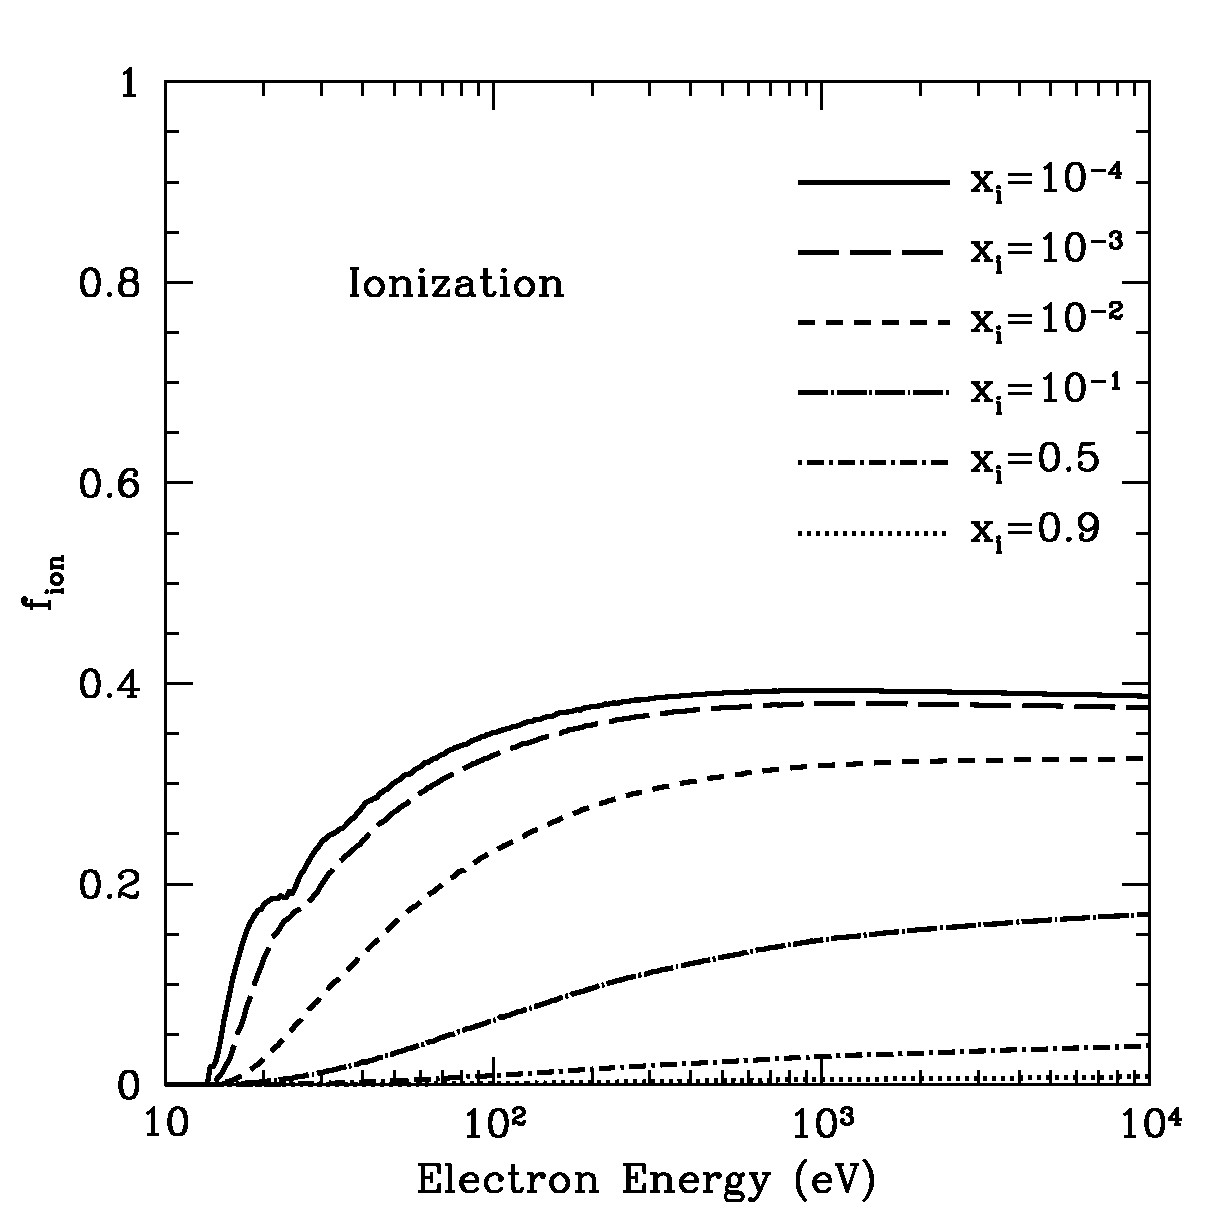
\includegraphics[width=0.4\textwidth]{Furlanetto/figure2-5a} 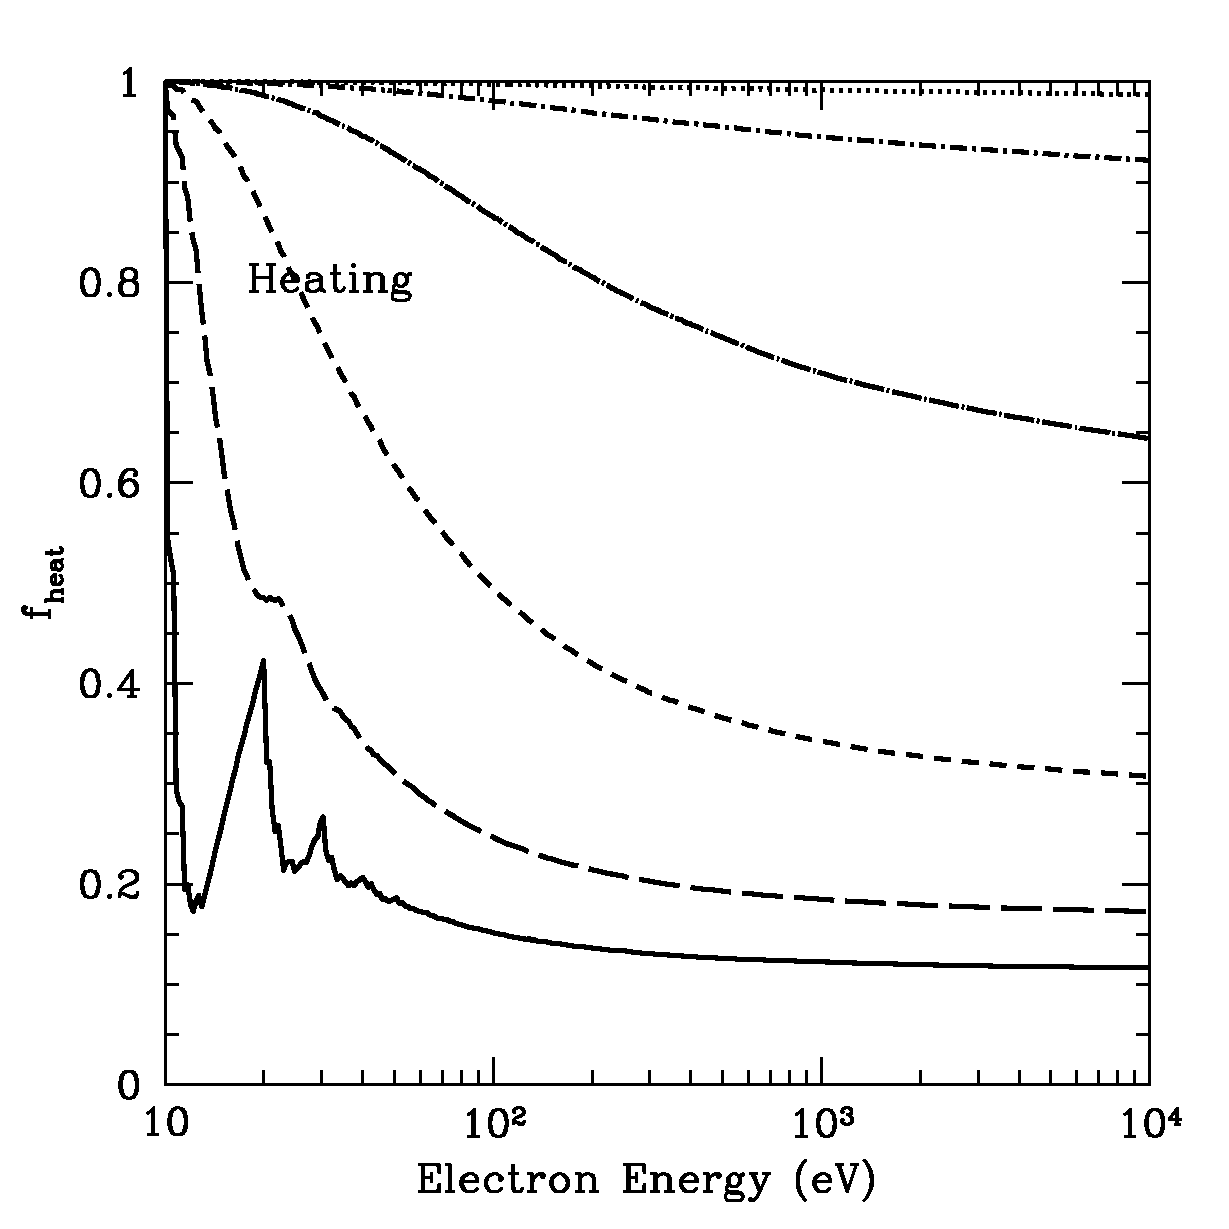
\includegraphics[width=0.4\textwidth]{Furlanetto/figure2-5b} \\
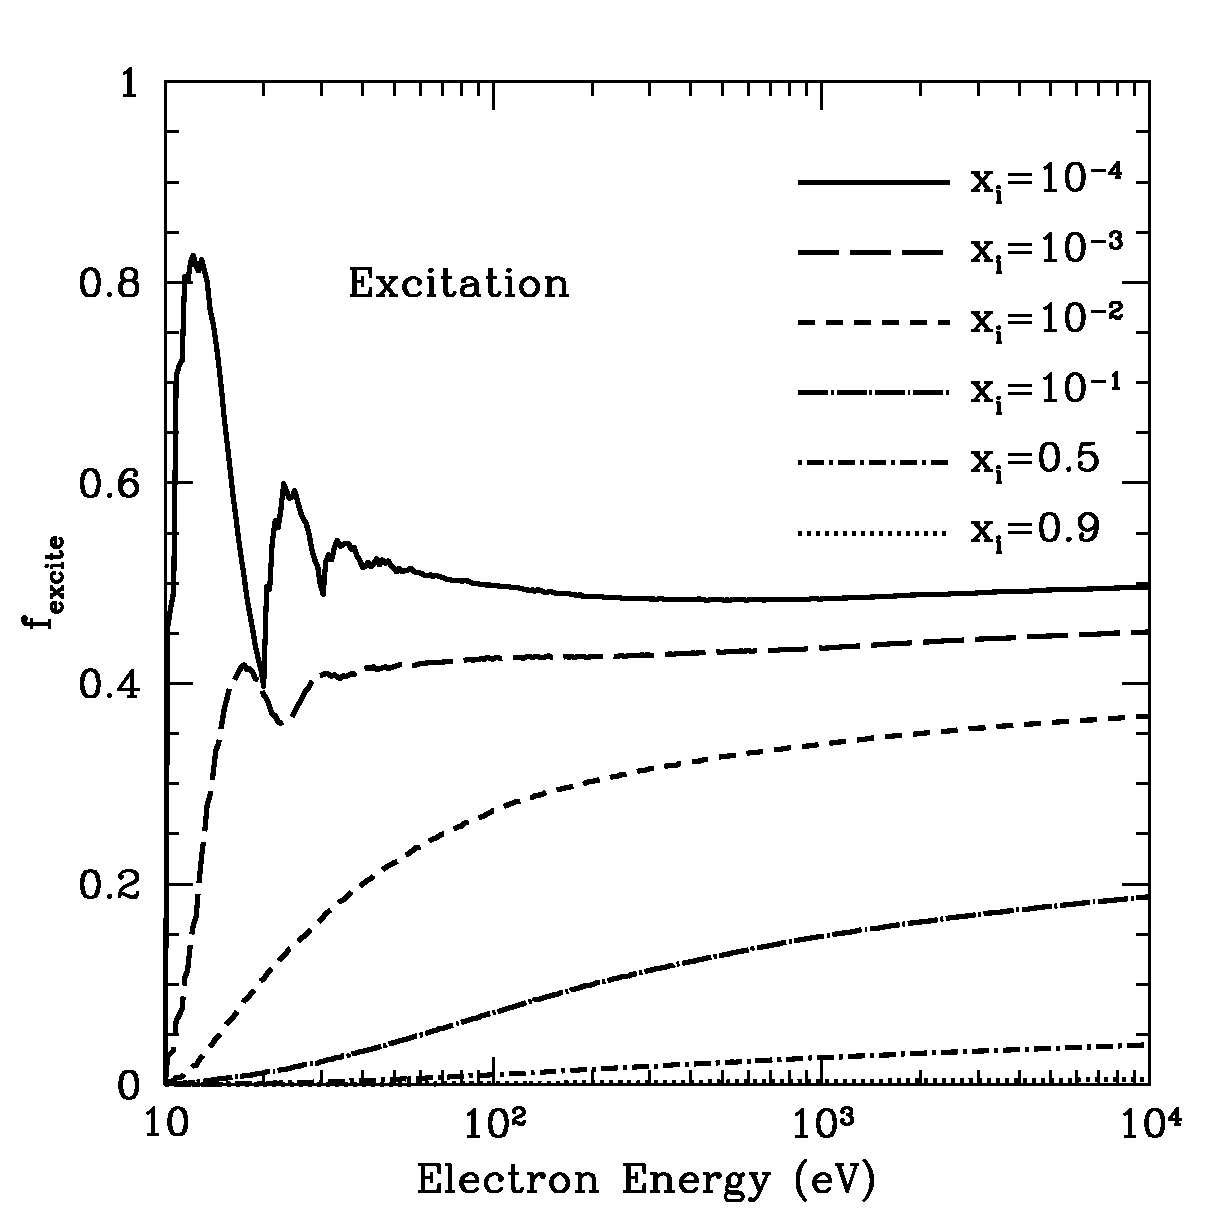
\includegraphics[width=0.4\textwidth]{Furlanetto/figure2-5c} 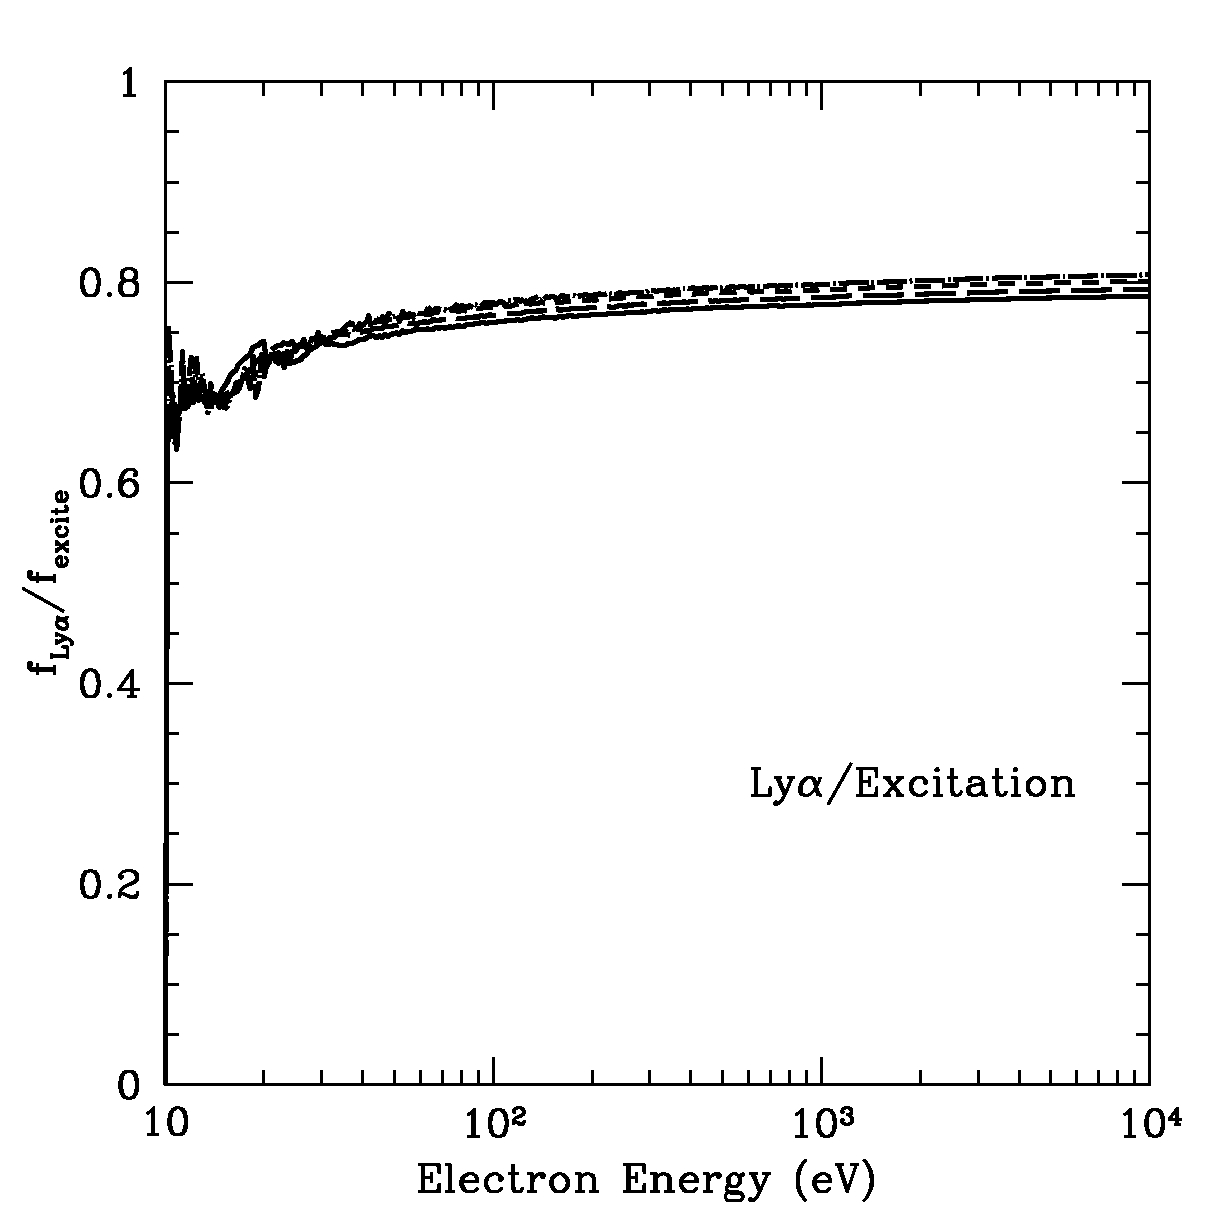
\includegraphics[width=0.4\textwidth]{Furlanetto/figure2-5d}
\end{center}
\caption{Energy deposition from fast electrons. We show the fraction of the initial energy deposited in ionization (upper left), heating (upper right), and collisional excitation (lower left), as a function of electron energy and for several different ionized fractions $x_i$. The lower right shows the fraction of the collisional excitation energy deposited in the HI Lyman-$\alpha$ transition, $f_{\rm Ly\alpha}$.  From \cite{furl10-xray}.}
\label{fig:xrayheat}
\end{figure}

The details of this process have been examined numerically \cite{shull85,valdes08,furl10-xray}, and Figure~\ref{fig:xrayheat} shows some example results. Note that the deposition fractions are smooth functions at high electron energies but, at low energies -- where the atomic energy levels become relevant -- can be quite complex. A number of approximate fits have been presented for the high-energy regime \cite{ricotti02, volonteri09}, but they are not accurate over the full energy range. A crude but useful approximation to the high-energy limit often suffices \cite{chen04-decay}:
\begin{eqnarray}
f_{\rm heat} & \sim & (1+2 x_i)/3 \nonumber \\
f_{\rm ion} \sim f_{\rm excite} & \sim & (1-x_i)/3,
\label{eq:fxapprox}
\end{eqnarray}
where $x_i$ is the ionized fraction. In highly ionized gas, collisions with free electrons dominate and $f_{\rm heat} \rightarrow 1$; in the opposite limit, the energy is split roughly equally between these three processes. However, the complexity of the behavior at low electron energies -- together with the increasing optical thickness of the IGM in that regime, and the fact that most sources are brighter in this soft X-ray regime -- suggest that a more careful treatment is needed for accurate work. \cite{furl10-xray} recommend interpolating the exact results.

\bibliographystyle{plain}
\bibliography{Furlanetto/ch2-refs}


\chapter{Chapter title}

\begin{bf}
  \author{Author Name}\\
  
Abstract\\
\end{bf}

This chapter discusses some important things


\section{A Section}

Lorem ipsum dolor sit amet, consectetur adipiscing elit. Duis eu egestas erat. Maecenas tincidunt lacinia tincidunt. Mauris id lectus nec neque feugiat condimentum vitae at diam. In vel orci nunc, non commodo mauris. Vivamus ipsum enim, vulputate quis pharetra non, molestie quis felis. Vivamus porttitor placerat turpis at accumsan. Nunc tortor velit, faucibus a rhoncus nec, blandit non elit. Nam consectetur lectus eu nisi blandit dapibus rhoncus dui tempus. Mauris fermentum dolor vel ipsum vulputate sit amet ultricies tortor lacinia. Donec ut nibh erat. Morbi nec mi ante. Integer nec vestibulum diam. Donec tincidunt pellentesque quam, ut interdum mauris venenatis condimentum. Nam condimentum, augue in aliquet gravida, neque dui elementum eros, id semper eros purus sed felis. Curabitur in justo sit amet sapien ultrices hendrerit at quis nibh. Quisque iaculis pulvinar tincidunt. 
\begin{eqnarray}
C(12) &= &\left[\overrightarrow{\pi}\cdot\overrightarrow{\phi}(x+r)\right] \nonumber \\ 
&\approx& 1-\mathrm{const}\frac{r^2}{L^2}\int_r^L\frac{x\rmd x}{x^2} + \cdots \nonumber  \\
&\approx& 1-\mathrm{const}\frac{r^2}{L^2}\ln\frac{x\rmd x}{x^2} + \cdots .\label{brokenlongeqn}
\end{eqnarray}

Aenean tellus risus, porta sit amet porta vitae, tincidunt ut felis. Class aptent taciti sociosqu ad litora torquent per conubia nostra, per inceptos himenaeos. Vestibulum ante ipsum primis in faucibus orci luctus et ultrices posuere cubilia Curae; Phasellus pulvinar placerat velit auctor egestas. Vivamus euismod fringilla tincidunt. Sed ut magna felis, id sollicitudin nunc. Quisque a dui eu erat consectetur egestas a quis justo. Aenean euismod congue diam, vel posuere urna fermentum sit amet. Lorem ipsum dolor sit amet, consectetur adipiscing elit. Mauris faucibus lacus eget est mollis auctor. Donec at nibh ligula, et posuere massa. Phasellus quis leo diam \cite{diamantaras1996pcn}.
Donec aliquam blandit risus, eu venenatis ante euismod eu. Curabitur cursus justo id arcu condimentum feugiat. Integer sapien urna, vulputate et adipiscing nec, convallis et justo. Suspendisse in ipsum at felis ornare interdum \cite{tulone2006pts},

\begin{figure}[]
\begin{center}

\includegraphics[width=0.5\textwidth]{Mirocha/01x01-eps-converted-to}
\end{center}
\caption{This is figure 1 in chapter 1.}
\end{figure}

\paragraph{Cras adipiscing} sagittis nunc vel luctus. Suspendisse volutpat augue quis erat semper consequat dignissim tellus euismod. Morbi hendrerit, tellus id aliquam iaculis, nibh leo tincidunt eros, vitae varius ligula felis in mi.

\begin{table}
\caption{Greek Letters.}
\begin{center}
\begin{tabular}{llllllll}
\hline
$\alpha $  & $ \beta $  & $ \gamma $  & $ \delta $  & $ \epsilon $  & $ \varepsilon $  & $ \zeta $  & $ \eta $ \\
 $ \theta $  &  $ \vartheta $  &  $ \gamma $  &  $ \kappa $  &  $ \lambda $  &  $ \mu $  &  $ \nu $  &  $ \xi $ \\
 $ o $  &  $ \pi $  &  $ \varpi $  &  $ \rho $  &  $ \varrho $  &  $ \sigma $  &  $ \varsigma $  &  $$ \\
 $ \tau $  &  $ \upsilon $  &  $ \phi$ &  $ \varphi $  &  $ \chi $  &  $ \psi $  &  $ \omega$  &  $ $ \\
 &  &  &  &  &  &  & \\
$ \Gamma $  & $ \Delta $  & $ \Theta $  &  $ \Lambda $  &  $ \Xi $  &  $ \Pi $  &  $ \Sigma $  & $ \Upsilon $ \\
 $ \Phi$ &  $ \Psi $  &  $ \Omega $  &  &  &  &  &\\
\hline
\end{tabular}
\end{center}\end{table}

\begin{figure}[]
\begin{center}

\includegraphics[width=0.6\textwidth]{Mirocha/01x02}
\end{center}
\caption{This is figure 2 in chapter 1.}
\end{figure}


\bibliographystyle{plain}
\bibliography{Mirocha/References}



\chapter{Physical cosmology from the 21-cm line}

\begin{bf}
  \author{Jonathan Pritchard}\\
  
a discussion of using 21-cm intensity mapping/interferometry to constrain the matter power spectrum and cosmological parameters.  The signal can also be used as a signpost for new physics beyond the standard model, such as heating and cooling of the primordial gas through interactions with dark matter.  Subtopics could include: redshift space distortions and their likely observability, measuring the matter power spectrum during the cosmic dawn and (eventually) the dark ages, IGM heating through dark matter annihilations, IGM cooling through interactions with exotic dark matter candidates.  \\
\end{bf}

This chapter discusses some important things

\section{Physical cosmology through the 21-cm epoch}
Summarise the different ways in which cosmology underpins the nature of the 21 cm signal.

\subsection{Dark matter} 
Discuss different dark matter models and impact

\subsection{PMBH}
Discuss primordial black holes and other exotic objects 

%%%%%
\section{Unique signatures of cosmology}
What might be distinctive signatures of cosmology in the 21cm signal?

\subsection{Non-Gaussianity} 
Impact of clustering on bubbles.

\subsection{IGM Heating} 
Various ways exotic physics can impact 21 cm signal

%%%%%
\section{Separating cosmology from astrophysics}
How might cosmology be separated from astrophysics?

\subsection{Redshift space distortions}
As route to separating different elements of signal

\subsection{Time evolution}
Looking at the dark ages, or via time evolution, or going to late times to post-EoR.

\section{Summary}

Lorem ipsum dolor sit amet, consectetur adipiscing elit. Duis eu egestas erat. Maecenas tincidunt lacinia tincidunt. Mauris id lectus nec neque feugiat condimentum vitae at diam. In vel orci nunc, non commodo mauris. Vivamus ipsum enim, vulputate quis pharetra non, molestie quis felis. Vivamus porttitor placerat turpis at accumsan. Nunc tortor velit, faucibus a rhoncus nec, blandit non elit. Nam consectetur lectus eu nisi blandit dapibus rhoncus dui tempus. Mauris fermentum dolor vel ipsum vulputate sit amet ultricies tortor lacinia. Donec ut nibh erat. Morbi nec mi ante. Integer nec vestibulum diam. Donec tincidunt pellentesque quam, ut interdum mauris venenatis condimentum. Nam condimentum, augue in aliquet gravida, neque dui elementum eros, id semper eros purus sed felis. Curabitur in justo sit amet sapien ultrices hendrerit at quis nibh. Quisque iaculis pulvinar tincidunt. 
\begin{eqnarray}
C(12) &= &\left[\overrightarrow{\pi}\cdot\overrightarrow{\phi}(x+r)\right] \nonumber \\ 
&\approx& 1-\mathrm{const}\frac{r^2}{L^2}\int_r^L\frac{x\rmd x}{x^2} + \cdots \nonumber  \\
&\approx& 1-\mathrm{const}\frac{r^2}{L^2}\ln\frac{x\rmd x}{x^2} + \cdots .\label{brokenlongeqn}
\end{eqnarray}

Aenean tellus risus, porta sit amet porta vitae, tincidunt ut felis. Class aptent taciti sociosqu ad litora torquent per conubia nostra, per inceptos himenaeos. Vestibulum ante ipsum primis in faucibus orci luctus et ultrices posuere cubilia Curae; Phasellus pulvinar placerat velit auctor egestas. Vivamus euismod fringilla tincidunt. Sed ut magna felis, id sollicitudin nunc. Quisque a dui eu erat consectetur egestas a quis justo. Aenean euismod congue diam, vel posuere urna fermentum sit amet. Lorem ipsum dolor sit amet, consectetur adipiscing elit. Mauris faucibus lacus eget est mollis auctor. Donec at nibh ligula, et posuere massa. Phasellus quis leo diam \cite{diamantaras1996pcn}.
Donec aliquam blandit risus, eu venenatis ante euismod eu. Curabitur cursus justo id arcu condimentum feugiat. Integer sapien urna, vulputate et adipiscing nec, convallis et justo. Suspendisse in ipsum at felis ornare interdum \cite{tulone2006pts},

\begin{figure}[]
\begin{center}

\includegraphics[width=0.5\textwidth]{Mirocha/01x01-eps-converted-to}
\end{center}
\caption{This is figure 1 in chapter 1.}
\end{figure}

\paragraph{Cras adipiscing} sagittis nunc vel luctus. Suspendisse volutpat augue quis erat semper consequat dignissim tellus euismod. Morbi hendrerit, tellus id aliquam iaculis, nibh leo tincidunt eros, vitae varius ligula felis in mi.

\begin{table}
\caption{Greek Letters.}
\begin{center}
\begin{tabular}{llllllll}
\hline
$\alpha $  & $ \beta $  & $ \gamma $  & $ \delta $  & $ \epsilon $  & $ \varepsilon $  & $ \zeta $  & $ \eta $ \\
 $ \theta $  &  $ \vartheta $  &  $ \gamma $  &  $ \kappa $  &  $ \lambda $  &  $ \mu $  &  $ \nu $  &  $ \xi $ \\
 $ o $  &  $ \pi $  &  $ \varpi $  &  $ \rho $  &  $ \varrho $  &  $ \sigma $  &  $ \varsigma $  &  $$ \\
 $ \tau $  &  $ \upsilon $  &  $ \phi$ &  $ \varphi $  &  $ \chi $  &  $ \psi $  &  $ \omega$  &  $ $ \\
 &  &  &  &  &  &  & \\
$ \Gamma $  & $ \Delta $  & $ \Theta $  &  $ \Lambda $  &  $ \Xi $  &  $ \Pi $  &  $ \Sigma $  & $ \Upsilon $ \\
 $ \Phi$ &  $ \Psi $  &  $ \Omega $  &  &  &  &  &\\
\hline
\end{tabular}
\end{center}\end{table}

\begin{figure}[]
\begin{center}

\includegraphics[width=0.6\textwidth]{Mirocha/01x02}
\end{center}
\caption{This is figure 2 in chapter 1.}
\end{figure}


\bibliographystyle{plain}
\bibliography{Mirocha/References}



\chapter{Inference from the 21cm signal}

\begin{bf}
  \author{Bradley Greig}\\
  
Abstract\\
\end{bf}

In the previous chapters we have discussed in-depth the astrophysical and cosmological information that is encoded by the cosmic 21-cm signal. However, once we have a measurement, how do we extract this information from the signal? This chapter focusses on the inference of the interesting astrophysics and cosmology once we obtain a detection of the 21-cm signal. 

Essentially, inference of the astrophysics can be broken down into three parts:
\begin{itemize}
\item[1.] \textbf{Compression of the observed data into a manageable dataset:} The observed 21-cm signal varies spatially as well as along the line-of-sight (frequency or redshift dimension) to provide a full three dimensional movie of the intergalactic medium in the early Universe. However, the signal is faint, requiring either statistical methods to sum the data in order to increase the signal-to-noise or sophisticated approaches to extract the faint signal directly. 
\item[2.] \textbf{An efficient method to model/simulate the 21-cm signal:} In order to interpret the observations and understand the astrophysical processes responsible, we must be able to produce physically motivated models capable of replicating the signal. Further, these must be as computationally efficient as possible in order to be able to realistically investigate the 21-cm signal.
\item[3.] \textbf{A robust probabilistic framework to extract the physics:} The observed 21-cm signal is dependent on numerous physical processes, which within our models or simulations are described by many unknown parameters. Further, these contain approximations in order to deal with the requisite dynamic range. We must be able to characterise our ignorance in a meaningful way in order to be truly able to infer the astrophysical processes of the epoch of reionisation and cosmic dawn.
\end{itemize}
\noindent
In this chapter we will focus on each separately, discussing the current state-of-the-art in inferring the 21cm signal.

\section{What do we actually measure?}

The 21-cm signal from the neutral hydrogen in the intergalactic medium is measured by its brightness temperature, $T_{\rm b}$. However, this cannot be measured directly, instead it is expressed as a brightness temperature contrast, $\delta T_{b}$, relative to the Cosmic Microwave Background (CMB) temperature, $T_{\rm CMB}$ \cite{Furlanetto:2006}: 
\begin{equation} \label{eq:delTb}
\delta T_{b}(\mathbf{x},\nu) \equiv T_{\rm b}(\mathbf{x},\nu) - T_{\rm CMB, 0}.
\end{equation}
As such, this brightness temperature contrast can be seen either in emission or absorption, dependent on the 21-cm brightness temperature which itself is dependent on the excitation state of the neutral hydrogen (i.e. its spin temperature, $T_{\rm S}$, see {\color{red} previous chapter}). We can re-express Equation~\ref{eq:delTb} in terms of $T_{\rm S}$ to recover {\color{red} (should have been introduced in a previous chapter)},
\begin{equation} \label{eq:delTb_Ts}
\delta T_{b}(\mathbf{x},\nu) \equiv \frac{T_{\rm S}(\mathbf{x},\nu) - T_{\rm CMB}(z)}{1+z} \left( 1 - {\rm e}^{-\tau_{\nu_{0}}(\mathbf{x},\nu) } \right),
\end{equation}
where $\tau_{\nu_{0}}$ is the optical depth of the 21-cm line. $\delta T_{b}(\mathbf{x},\nu)$ varies spatially due to its two-dimensional angular position on the sky while it varies along the line-of-sight direction owing to the 21-cm line being redshifted by cosmological expansion (i.e. adding a frequency or time dependence to the signal). Thus, measuring $\delta T_{b}(\mathbf{x},\nu)$ can reveal a full three-dimensional movie of the neutral hydrogen in the early Universe.

Unfortunately, $\delta T_{b}(\mathbf{x},\nu)$ is faint. Further, in reality it is buried under numerous astrophysical foregrounds all of which are orders of magnitude brighter {\color{red} (see relevant chapters for more detailed discussions)}. In order to deal with this faint signal coupled with the astrophysical foregrounds, typically we seek to compress the data to boost the signal-to-noise or specifically tailor methods to extract the faint signal. In this chapter, we will discuss the numerous methods proposed in order to tease out the faint astrophysical signal from the noise.

\section{Optimal methods for characterising the 21-cm signal}

The first step in our efforts to be able to infer information about the astrophysical processes responsible for reionisation and the cosmic dawn is to explore optimal methods to characterise the 21-cm signal. In this section, we summarise the wide variety of approaches considered in the literature, highlighting the leverage that each is able to provide with respect to the underlying astrophysical processes. Note that throughout this chapter, all investigations into detecting the 21-cm signal are generated theoretically, either analytically or numerically. Thus, we urge the reader to refer to the citations in order to understand the limiting assumptions.

\subsection{Global signal} \label{sec:global}

The simplest way to deal with such a faint signal is to average it over as large a volume as possible. Since the 21-cm signal is visible across the entire sky, one can produce a complete sky-averaged (global) 21-cm brightness temperature as a function of frequency (redshift). Although the two-dimensional spatial information from the 21-cm signal is lost, the main advantage is that it is relatively cheap to observe, requiring comparatively simple instrumentation {\color{red} (see future chapter on global signal or observations?)}. A fact that several experiments have used in an attempt to provide a measurement of the 21-cm signal, given that a single radio dipole is capable of seeing essentially the entire sky at any one time. In Figure~\ref{fig:global}, we show a representative model of the global 21-cm signal, highlighting the major cosmological milestones that have been discussed in previous chapters. Thus, in each frequency bin, we measure an all-sky average of the 21-cm brightness temperature.

\begin{figure}[]
\begin{center}
%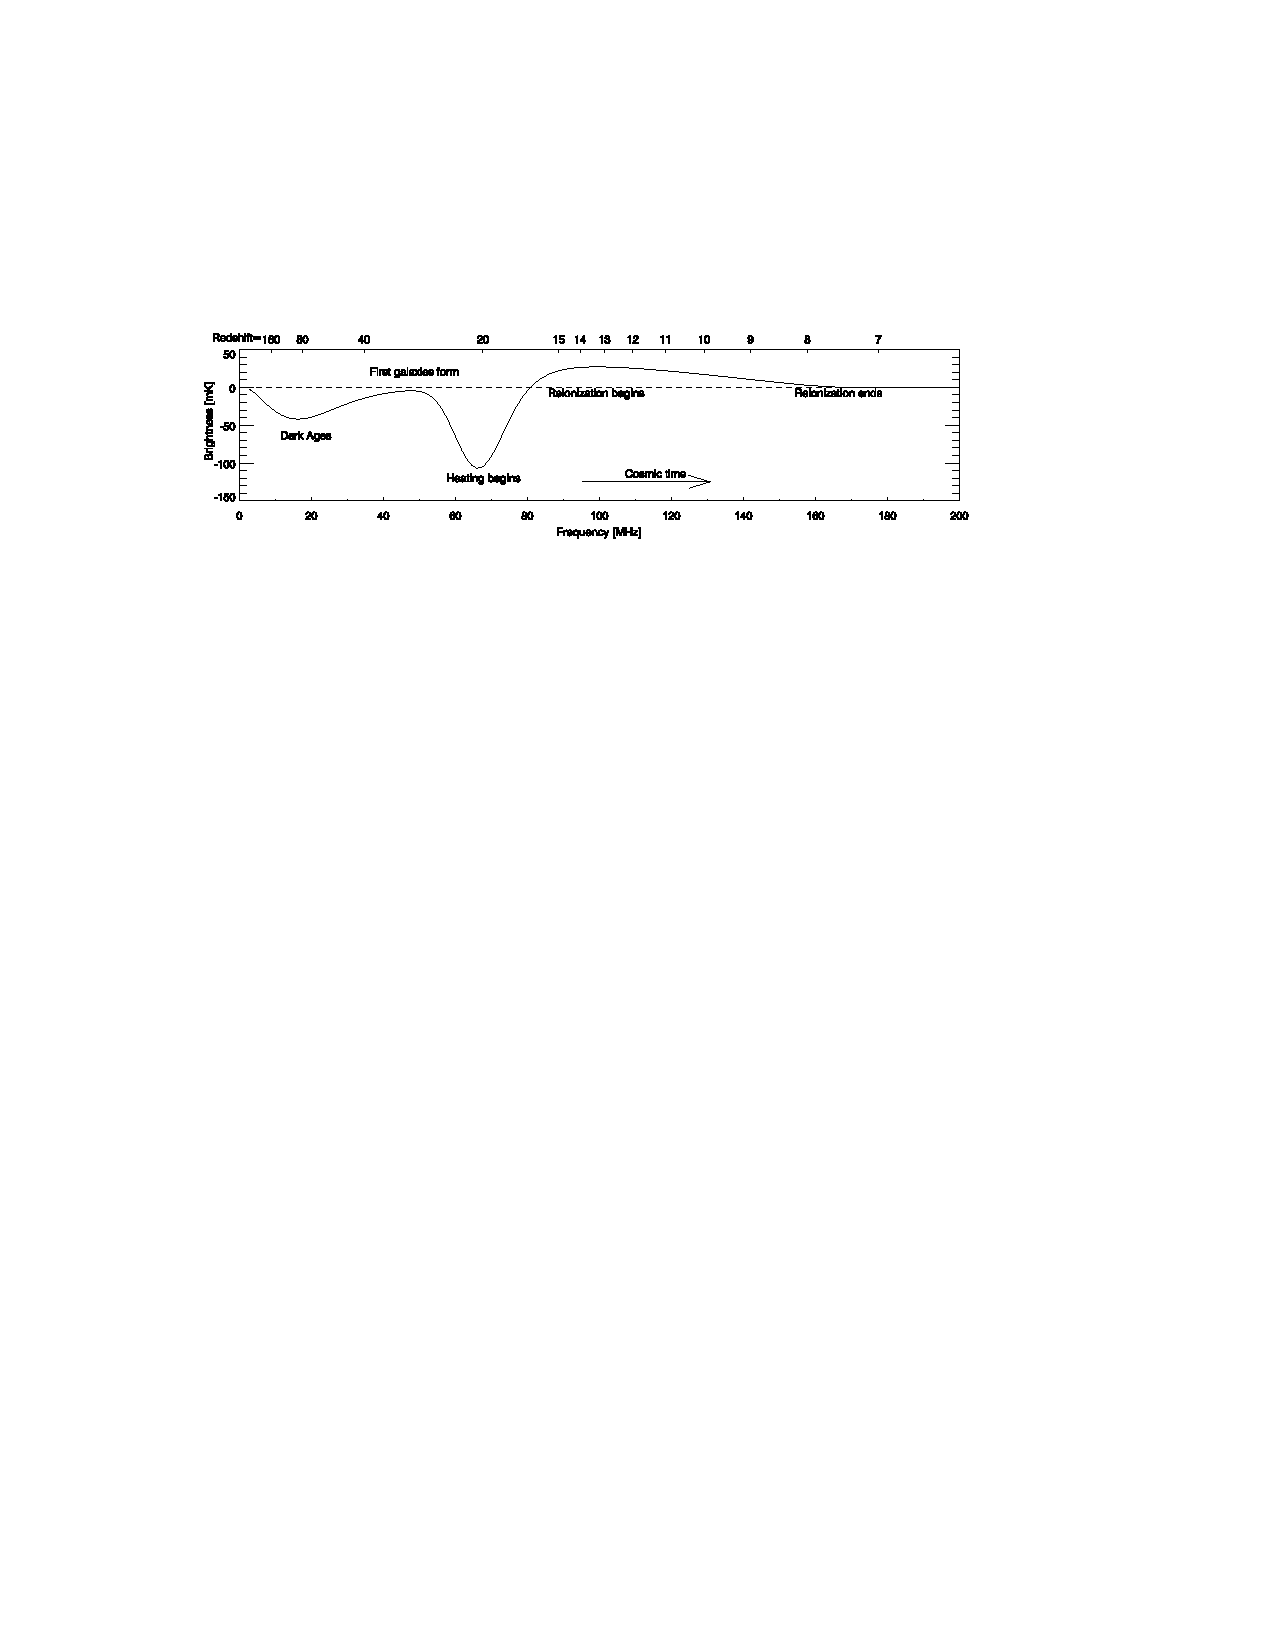
\includegraphics[width=1.\textwidth]{Greig/GlobalSignal}
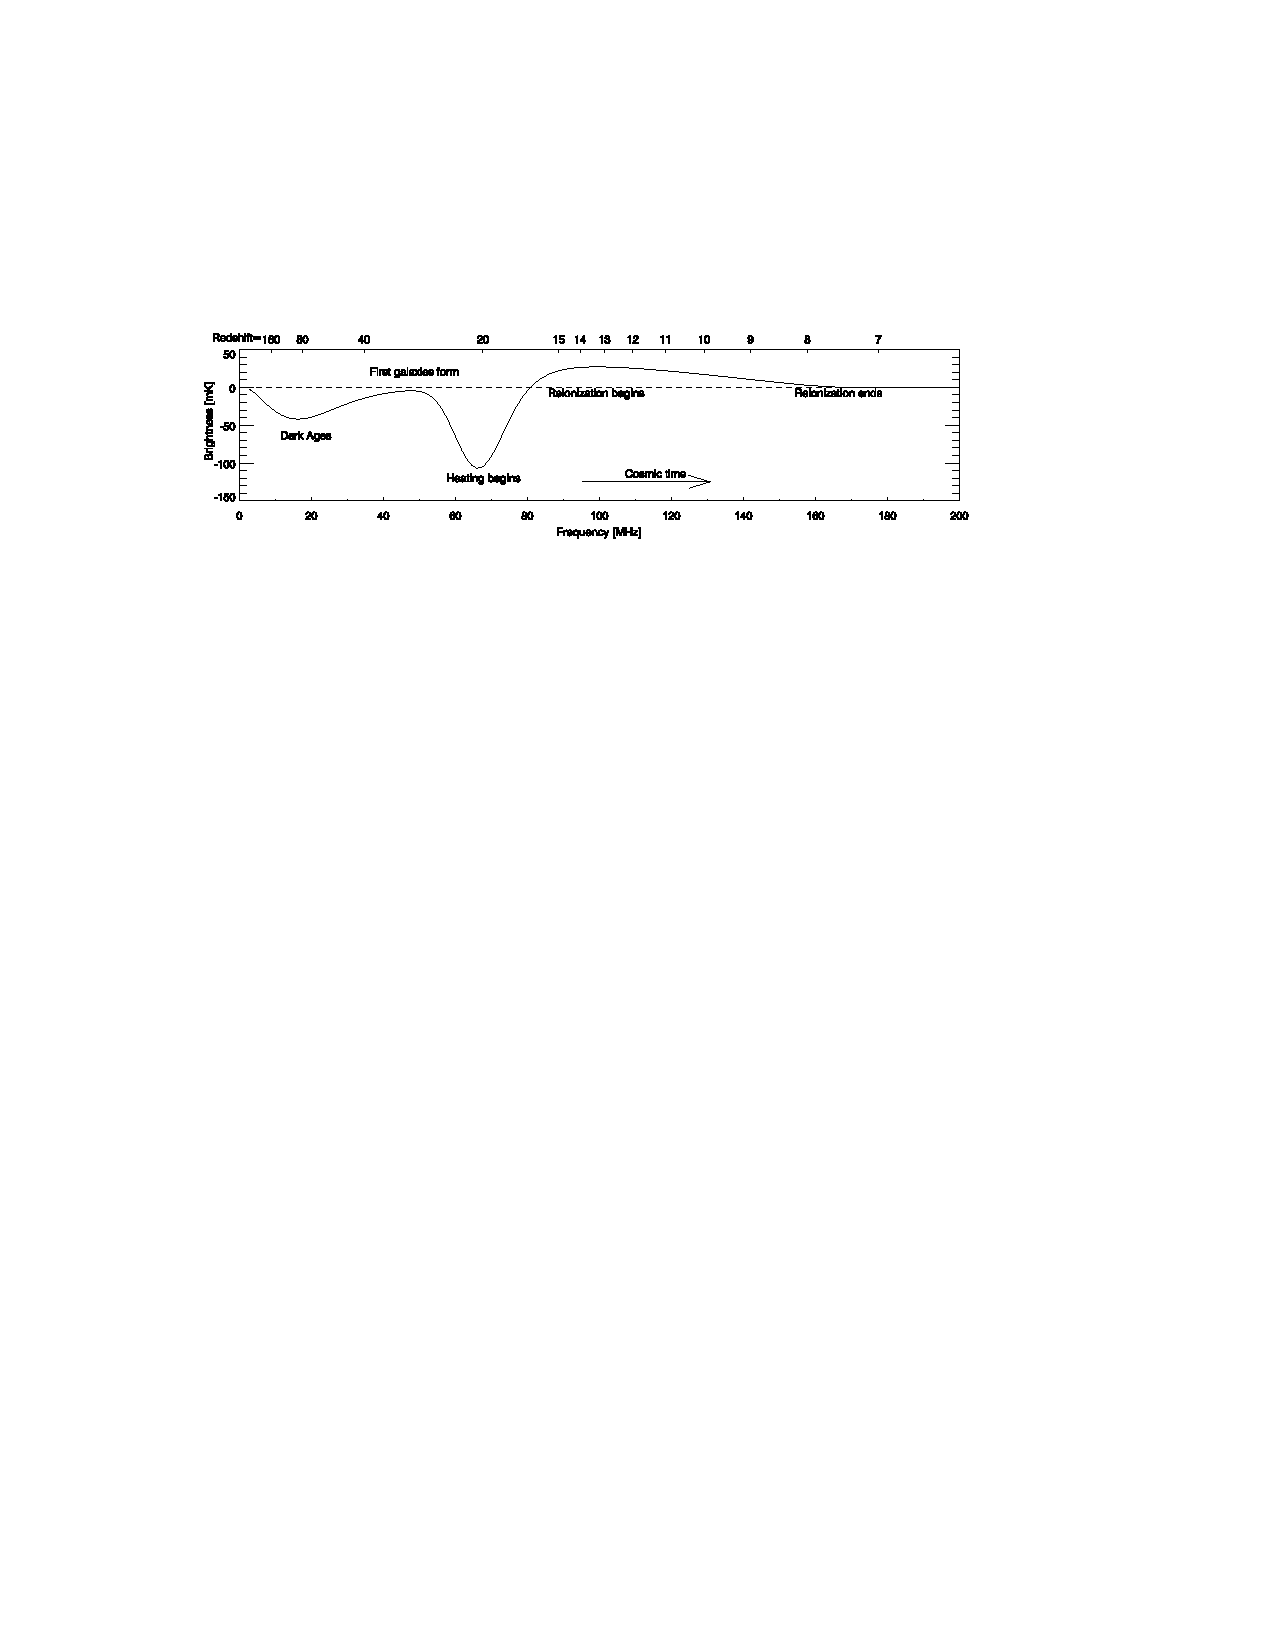
\includegraphics[trim = 0.2cm 0.6cm 0.2cm 0.2cm, scale = 1.0]{Greig/GlobalSignal}
\end{center}
\caption{A representative example of the all-sky averaged (global) 21-cm brightness temperature signal, demarcating the major cosmological transitions. Taken from \cite{Pritchard:2012}.}
\label{fig:global}
\end{figure}

The global signal has been studied extensively in the literature. {\color{red} Use this hook here to add in citations to works investigating the global signal}.

Roughly speaking the global 21-cm signal can be broken up into five major turning points (e.g. \cite{Furlanetto:2006,Pritchard:2010}) corresponding to: (i) a minimum during the dark ages where collisional coupling becomes ineffective, (ii) a maximum at the transition from the dark ages to the Ly$\alpha$ pumping regime (Ly$\alpha$ pumping from the first sources becomes efficient), (iii) a minimum at the commencement of X-ray heating taking the signal back towards emission, (iv) a maximum once the 21-cm signal becomes saturated during the EoR and finally (v) when reionisation is complete. Importantly, both the amplitude of the 21-cm signal as well as the frequency (redshift) of these transitions is strongly dependent on the underlying astrophysical processes. Thus, measuring both the amplitude and frequency of the turning points can reveal information into the underlying astrophysics.

In \cite{Mirocha:2013}, these authors connect these transitions more closely to the astrophysics. The second turning point (end of the dark ages) can, under certain simple assumptions, be used to place limits on the spin temperature, $T_{\rm S}$. Details on $T_{\rm S}$, through equation ({\color{red} should be in an earlier chapter}) can provide an estimate on the angle-averaged intensity of Ly$\alpha$ photons, $J_{\alpha}$. This provides insight into both the number density of sources and their corresponding emission spectrum (e.g. PopIII stars). The relative depth of the third turning point (heating epoch) can be used to place limits on the co-moving heating rate density, that is, the amount of heating that the IGM has undergone owing to heating sources (e.g. X-rays from HMXBs, the ISM or other more exotic scenarios {\color{red} should be discussed in an earlier chapter}). Again, distinguishing the number density and type of sources responsible. Finally, the saturation of the spin temperature, $T_{\rm S}$, during the epoch of reionisation collapses the brightness temperature into an approximate proportionality ({\color{red} cite appropriate equation}, $T_{\rm S} \propto x_{\rm H{\scriptstyle I}}(1+\delta_{\rm nl})$) with the underlying ionisation fraction, $x_{\rm H{\scriptstyle I}}$. Tracking the evolution of the ionised fraction, i.e. the reionisation history, reveals the time-span of reionisation. This reveals insights into the number density of ionising photons produced, and thus the types of sources responsible for reionising the Universe.

Up until very recently, the first transition was typically ignored, as it was assumed that this transition was well understood theoretically. That is, that the dark matter and baryons decoupled from the CMB temperature at the same time, both cooling adiabatically. It turns out that the dark matter decouples earlier than the baryons, meaning the dark matter is colder than the baryons. As such, the baryons can be cooled by a coupling between the dark matter and baryons (e.g. \cite{Tashiro:2014}) altering the amplitude of the 21-cm signal. In addition to this, relative velocity differences between the two fluids (dark matter and baryons) will affect the structure formation on small-scales (e.g. \cite{Tseliakhovich:2010}) again impacting on the temperature of the baryons. These will result in observable differences in the location and amplitude of this first turning point in the global signal, enabling dark matter models to be distinguishable (e.g. \cite{Munoz:2015,Fialkov:2018}).

To highlight the expected variation in the global 21-cm signal as a result of the underlying astrophysical processes, in Figure~\ref{fig:global_vary} we show $\sim~200$ theoretical models of the global 21-cm signal from \cite{Cohen:2017}. Here, the authors explore the maximal variation in the global 21-cm signal when varying the ionisation and heating properties of the astrophysical sources. Some common features in the signal are, the depth of the absorption trough deepens for lower X-ray luminosities (including some models which never appear in emission as a result of inefficient heating) or the turning points push to later times when the minimum masses of sources increases (i.e. require more massive haloes in which stars can form and produce ionising photons).

\begin{figure}[]
\begin{center}
%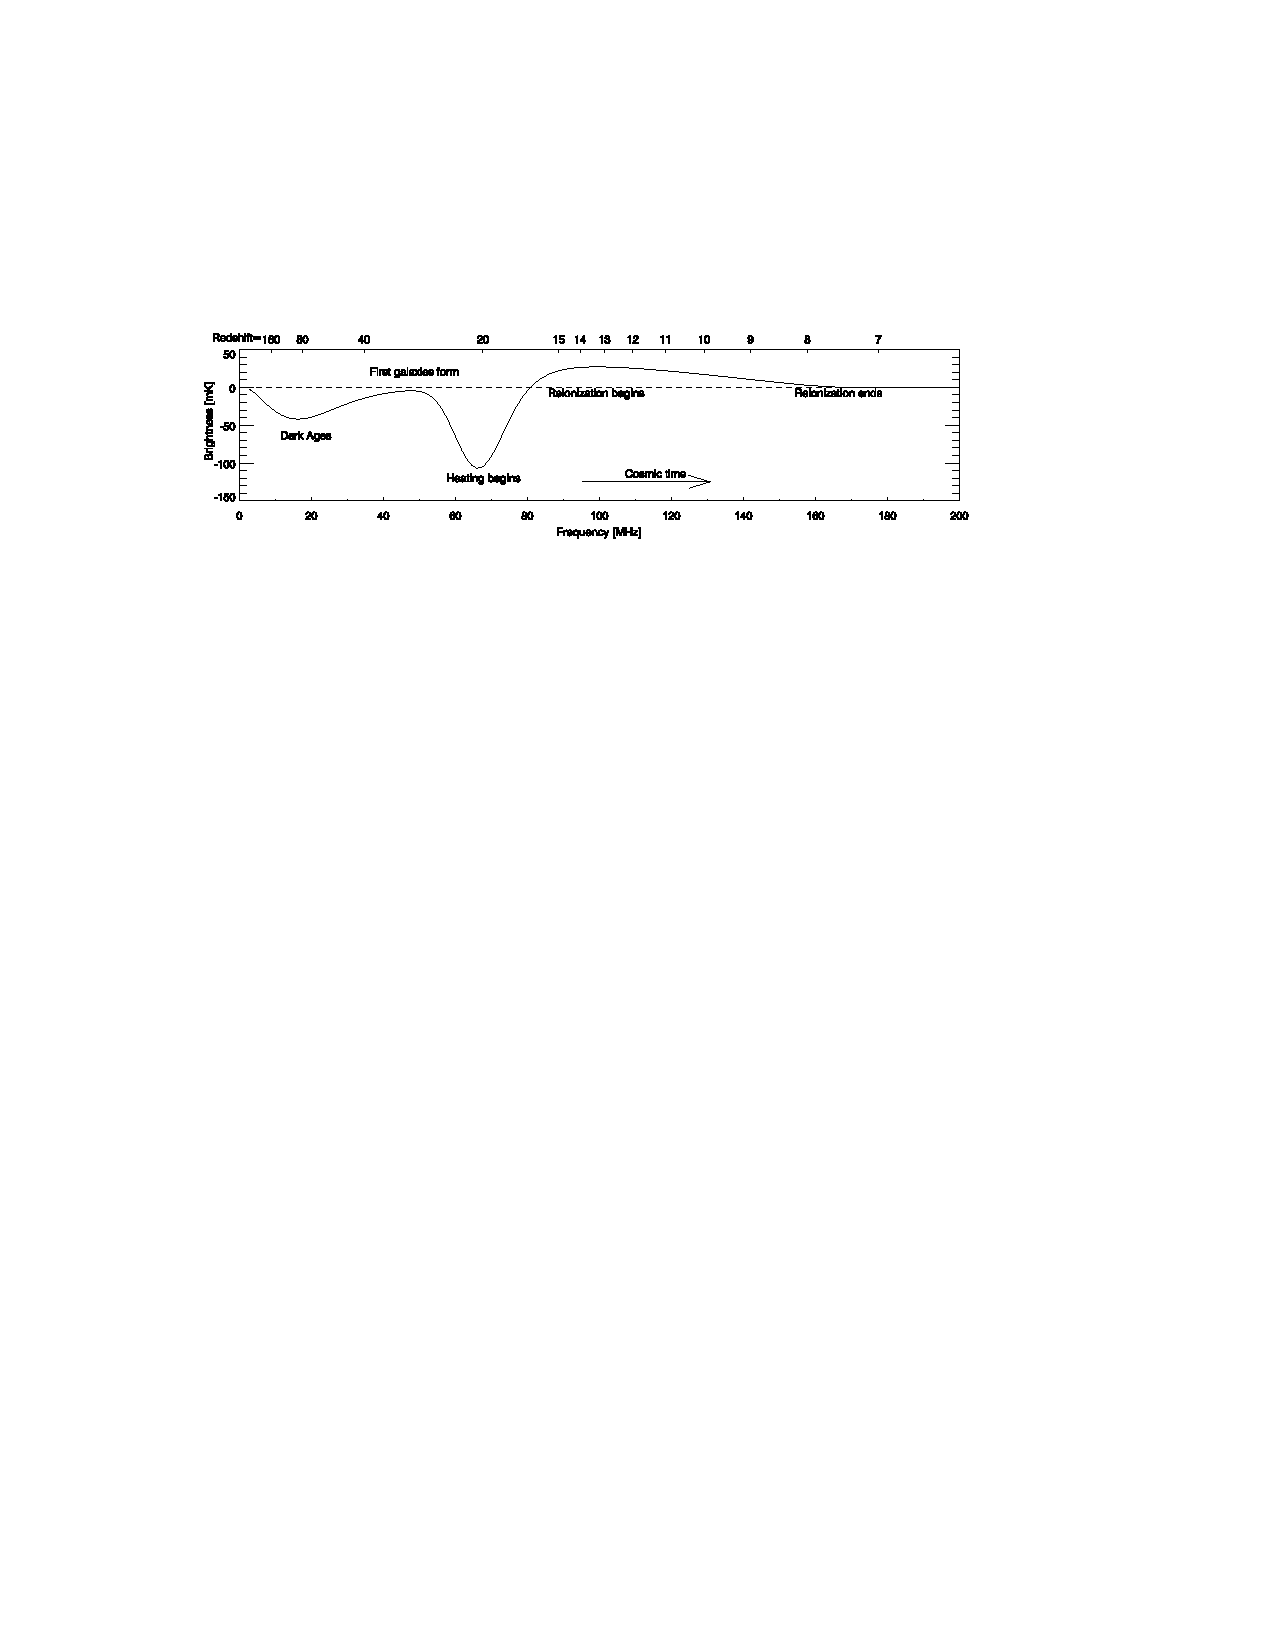
\includegraphics[width=1.\textwidth]{Greig/GlobalSignal}
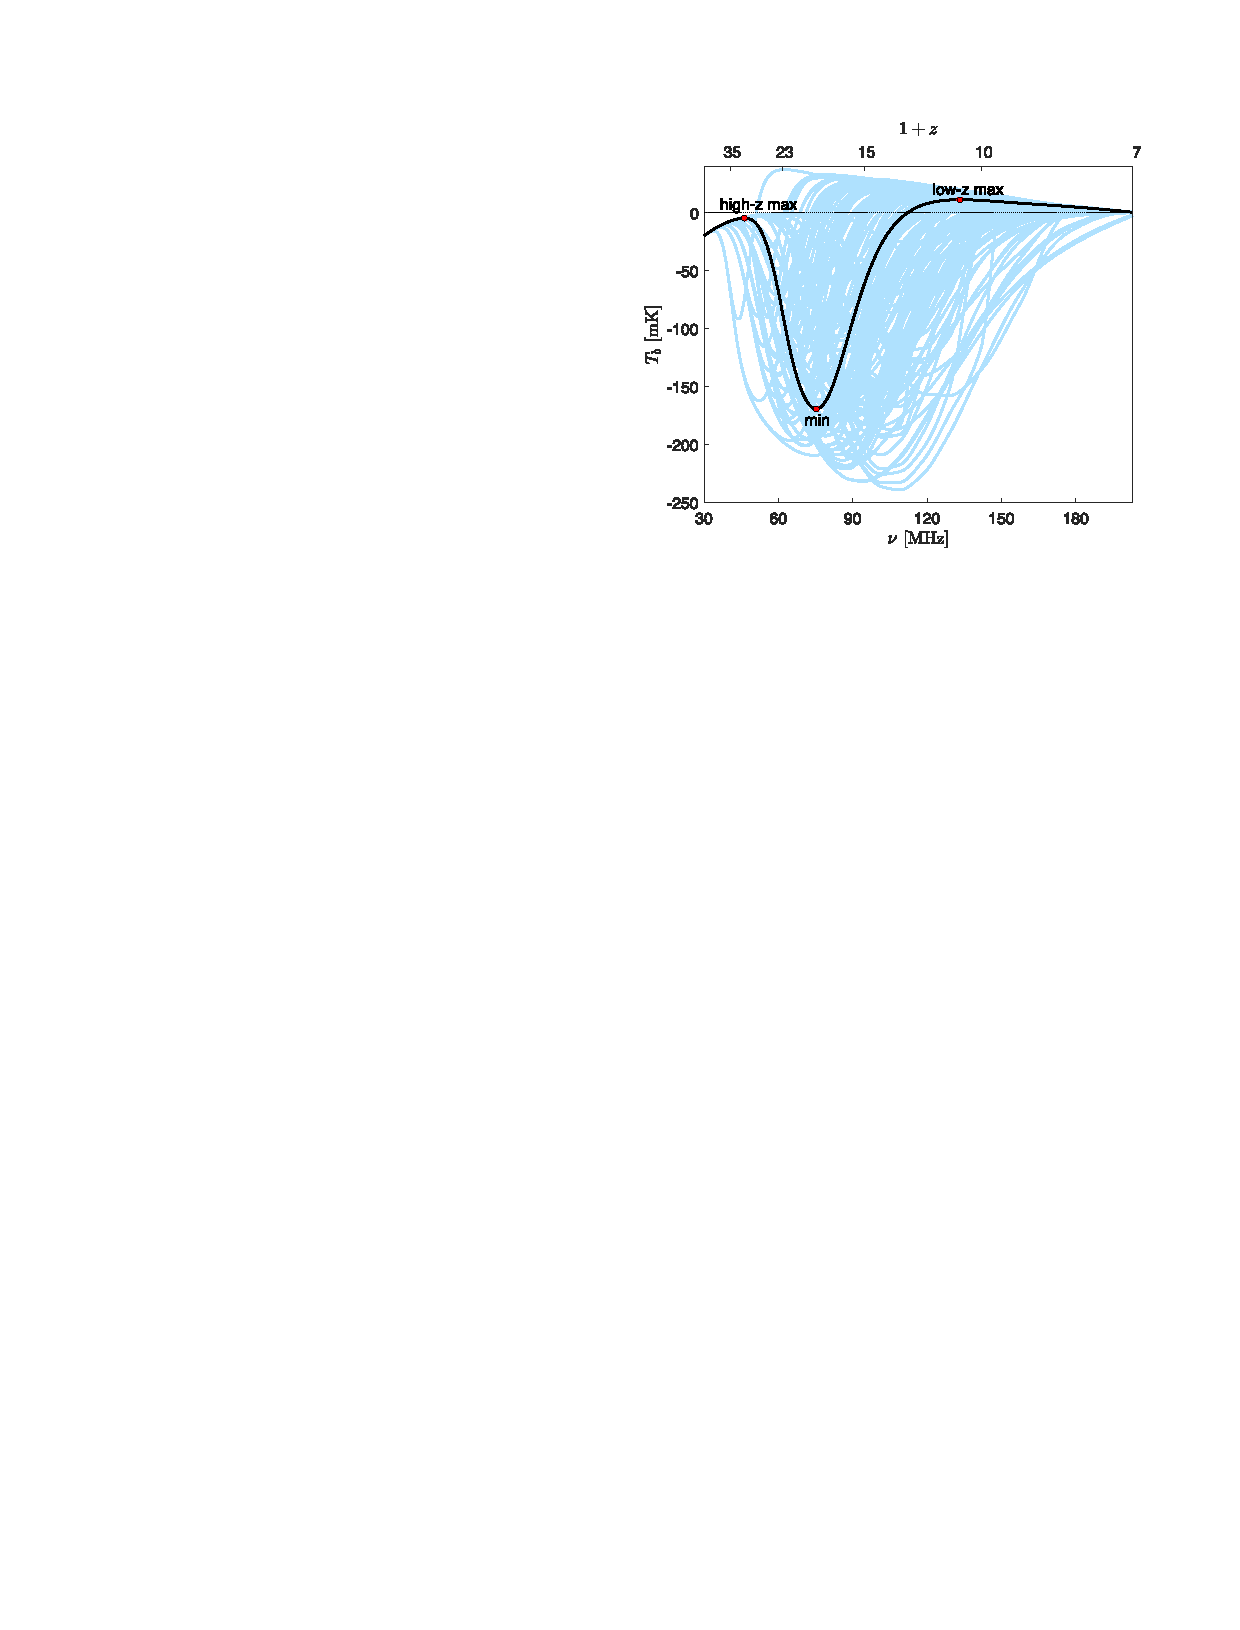
\includegraphics[trim = 0.2cm 0.6cm 0.2cm 0.2cm, scale = 0.9]{Greig/GSVariation}
\end{center}
\caption{The all-sky averaged (global) 21-cm brightness temperature signal obtained when varying the astrophysical parameters in $\sim~200$ theoretical models from \cite{Cohen:2017}.
}
\label{fig:global_vary}
\end{figure}

\subsection{Power spectrum}

After the global signal, the next simplest and most straightforward approach to characterise the 21-cm signal is through the power spectrum. This is the Fourier transform of the 2-point correlation function. Basically, a measure of the excess signal (above random) on all possible spatial scales. The workhorse statistic for any signal containing structural information, the power spectrum is simply the number of modes (in Fourier space) as a function of physical scale (or size). It produces a distribution of modes characterising the amount of structural information which is contained within the signal. The power spectrum is the natural method for observing the 21-cm signal from a radio interferometer, since these measure differences in the arrival times of the cosmological signal between radio dipoles or dishes of some fixed separation. Thus, a radio interferometer is sensitive to the spatial fluctuations rather than the total amplitude.

To obtain the 21-cm power spectrum, we normalise the 21-cm brightness temperature, $\delta T_{b}(\mathbf{x})$ to be a zero-mean quantity, $\delta_{21}(\mathbf{x}) = (\delta T_{b}(\mathbf{x}) - \delta\bar{T_{b}})/\delta\bar{T_{b}}$, which amplifies the fluctuations (spatial information) in the signal. The power spectrum, $P(\mathbf{k})$ is computed by the angle-averaged sum of the Fourier transform of the 21-cm brightness temperature fluctuations via,
\begin{eqnarray}
\langle \delta_{21}(\mathbf{k}_{1})\delta_{21}(\mathbf{k}_{2}) \rangle = (2\pi)^{3}\delta_{D}( \mathbf{k}_{1} + \mathbf{k}_{2})P(\mathbf{k}_{1}),
\end{eqnarray}
where $\delta_{D}$ is the Dirac delta function. Typically, the 21-cm power spectrum is converted into a dimensionless quantity through $\Delta^{2}(\mathbf{k}) = (k^{3}/2\pi^{2})P(\mathbf{k})$. Typically, the Fourier modes are then averaged in spherical shells to obtain the spherically averaged power spectrum, $P(k)$, which considerably improves the overall signal-to-noise, at the cost of averaging over some spatial information. Alternatively, one can also measure the two-dimensional cylindrically averaged power spectrum, $P(k_\parallel,~k_\perp)$ decomposing it into modes perpendicular to the line-of-sight ($k_\perp$; spatially averaging the two dimensional angular modes on the sky in annuli) and along the line-of-sight ($k_\parallel$; in frequency) direction. The strength of the two dimensional 21-cm power spectrum is that most of the contamination of the signal by the astrophysical foregrounds can be contained in what is referred to as the EoR `wedge' while the remaining Fourier modes can be clean tracers of the cosmological signal ({\color{red} cite references and/or subsequent chapter}).

The advantage of the power spectrum over the global signal, is that it provides a measure of the spatial fluctuations in the 21-cm signal. However, it does not encode all the available spatial information from the 21-cm signal. The power spectrum is a measure of how Gaussian the fluctuations are. If these fluctuations were truly Gaussian, the power spectrum would contain all the information, and any higher order $n$-point correlation functions would contain no additional information. The structural complexity of the large and small scale processes of reionisation and the cosmic dawn results in the signal being highly non-Gaussian. As such, the power spectrum does not reveal all available information, meaning there is further constraining power from the higher order $n$-point statistics. In section~\ref{sec:bispectrum} we will return to this. Nevertheless, the power spectrum still contains a wealth of information, and observationally is considerably easier to measure.

\begin{figure}[]
\begin{center}
%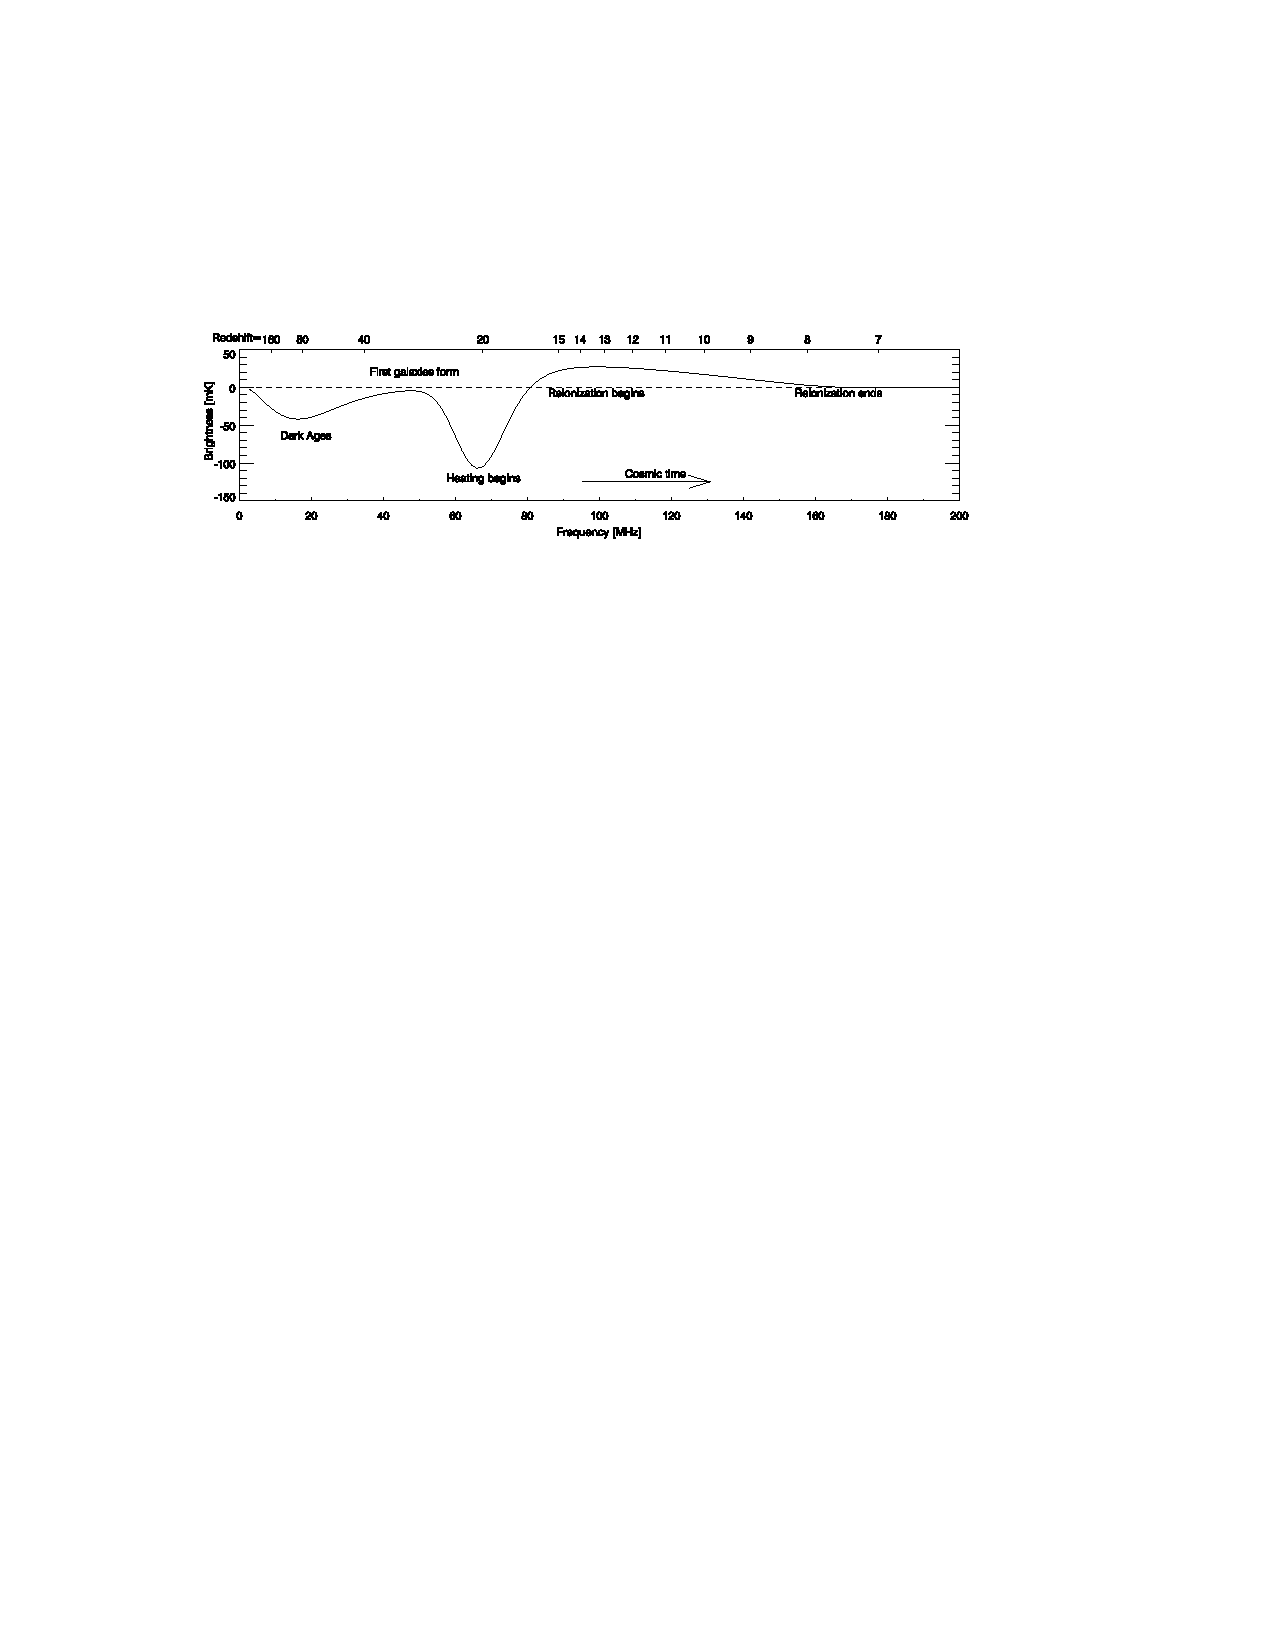
\includegraphics[width=1.\textwidth]{Greig/GlobalSignal}
\includegraphics[trim = 0.2cm 0.6cm 0.2cm 0.2cm, scale = 0.4]{Greig/PSMilestones}
\end{center}
\caption{The 21-cm power spectrum amplitude for two different Fourier modes, $k=0.1$~Mpc$^{-1}$ (solid) and $k=0.5$~Mpc$^{-1}$ (dashed). Peaks in the 21-cm power spectrum amplitude correspond to the different cosmic milestones. Taken from \cite{Mesinger:2016}.}
\label{fig:PSMilestones}
\end{figure}

The sensitivity of the 21-cm power spectrum to the underlying astrophysics can be highlighted when we decompose the 21-cm brightness temperature fluctuations through a perturbative analysis. In doing so, we can recover the following (see e.g. {\color{red} needs references}),
\begin{eqnarray}
\delta_{21} \propto C_{b}\delta_{b} + C_{x}\delta_{x} + C_{\alpha}\delta_{\alpha} + C_{T}\delta_{T} - \delta_{\partial v},
\end{eqnarray}
Simply put, fluctuations in the 21-cm brightness temperature field, $\delta_{21}$, are driven by a sum of contributions from the underlying density field, $\delta_{b}$, the ionisation fraction $\delta_{x}$, the Ly$\alpha$ coupling co-efficient, $\delta_{\alpha}$, the temperature of the neutral hydrogen $\delta_{T}$ and line-of-sight peculiar velocity gradient, $\delta_{\partial v}$. Computing the power spectrum then measures the combined signal from the power spectra of each field as well as the cross-power spectra of each. Thus, if we measure the 21-cm power spectrum across cosmic time, we will be sensitive to both the epochs when each component dominates (similar to the global signal) and also the spatial scales on which the signal is strongest. This, similar to the global signal is depicted in Figure~\ref{fig:PSMilestones}.

However, rather than using one single Fourier mode, we have a range of spatial scales over which to recover astrophysical information. This provides access to both the small-scale and large-scale physical processes. For example, during the EoR, the 21-cm power spectrum is dominated by the contribution from the ionisation field, which contains particular structural information on the reionisation process due to the characteristic size of the H$_{\rm \scriptsize II}$ regions as well as their clustering ({\color{red} cite references}). Similar is true for both the heating or Ly$\alpha$ coupling epochs, whereby the structural information provides insights into the intensity of the radiation, and the number density of sources producing it.

\begin{figure}[]
\begin{center}
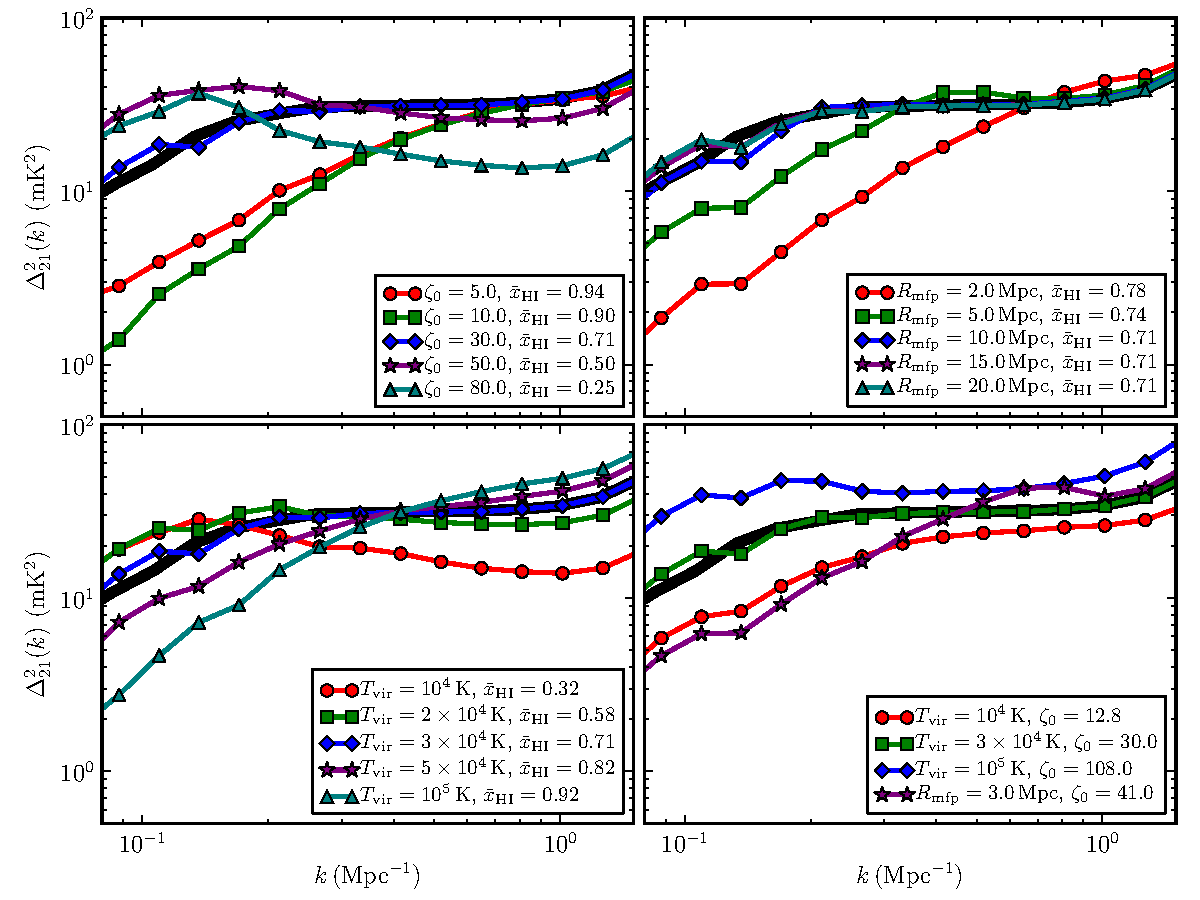
\includegraphics[trim = 0.2cm 1cm 0.2cm 0.2cm, scale = 0.75]{Greig/ParameterVariation_z9_0_book}
\end{center}
\caption{The three dimensional spherically averaged 21-cm power spectrum at $z=9.0$ when varying astrophysical parameters controlling different astrophysical processes, assuming $T_{\rm S} \gg T_{CMB}$~(\cite{Greig:2015}). Top left: the number of ionising photons produced per baryon (ionising efficiency, $\zeta$), top right: maximum ionising photon horizon (proxy for maximum allowable bubble size, $R_{\rm mfp}$) and bottom left: minimum mass of halo hosting star-forming galaxy (represented here as $T_{\rm vir}$). Bottom right: several models at the same ionisation fraction.}
\label{fig:PSvariation}
\end{figure}

In Figure~\ref{fig:PSvariation} we show the variation in the three dimensional spherically averaged 21-cm power spectrum at a single redshift ($z=9$) when varying three different astrophysical parameters under the assumption of $T_{\rm S} \gg T_{CMB}$(see e.g. \cite{Greig:2015}). Inset tables correspond to the parameter being varied and the resultant IGM neutral fraction (stage of reionisation). In the top left panel, we vary the ionising efficiency, $\zeta$, a proxy for the number of ionising photons produces by the sources. The shape of the 21-cm power spectrum differs considerably with ionising efficiency. In the early stages, the 21-cm PS matches the density (matter) power spectrum, while in the latter stages its follows the ionisation field {\color{red} this surely has been discussed in detail already and I don't have to elaborate on it?}. 

Similar behaviour is observed for varying $T_{\rm vir}$, a proxy for the minimum mass of halos hosting star-forming galaxies. Increasing this threshold, results in fewer sources to contribute to reionisation. In the top right panel, the maximum photon horizon, $R_{\rm mfp}$, is varied. Essentially, in this specific work it acts as a maximum allowable bubble size. Note that in this case, the change in $R_{\rm mfp}$ does not alter the neutral fraction strongly, thus the changes in the 21-cm power spectrum are purely as a result in changes to the size of the ionised regions. Finally, in the bottom right we highlight astrophysical models with the same IGM neutral fraction (i.e. the same stage of reionisation). Despite being at the same point in reionisation, the amplitude and shape of the 21-cm power spectrum differs considerably, highlighting the sensitivity of the 21-cm power spectrum to the underlying astrophysical parameters. 

While this example is only for the epoch of reionisation, the same strong sensitivity of the 21-cm power spectrum to the underlying astrophysics is true for both the heating or Ly$\alpha$ coupling epochs (see e.g. {\color{red} citations}). This highlights the strength and utility of the 21-cm power spectrum for recovering the astrophysical information. As such numerous authors have explored the impact of various astrophysical processes on the 21-cm power spectrum. {\color{red} refer to a variety of papers here, and potentially highlight the specific process used}.

\subsection{Bispectrum} \label{sec:bispectrum}

The logical extension beyond the power spectrum, the bispectrum, $B$, is simply the Fourier transform of the 3-point correlation function,
\begin{eqnarray}
\langle \delta_{21}(\mathbf{k}_{1})\delta_{21}(\mathbf{k}_{2})\delta_{21}(\mathbf{k}_{3}) \rangle = (2\pi)^{3}\delta_{D}( \mathbf{k}_{1} + \mathbf{k}_{2} + \mathbf{k}_{3})B(\mathbf{k}_{1},\mathbf{k}_{2},\mathbf{k}_{3}),
\end{eqnarray}
where the $\delta_{D}$ enforces that the Fourier modes must form closed triangles. It measures the excess probability of the underlying quantity as a function of three spatial positions in real space. The bispectrum provides a scale-dependent measure of the non-Gaussianity of the 21-cm signal, and as such contains additional astrophysical information beyond that held in the power spectrum. However, it suffers from lower signal-to-noise as there are less modes to average over to boost the signal.

Whereas the power spectrum is relatively trivial to interpret as it is a measure of the power over a single length scale, $k$, the bispectrum is the measure of power over all possible triangle configurations that satisfy the closure condition from $\delta_{D}$. Thus in order to simplify the interpretation of the bispectrum, it is common to consider several simplified triangle configurations. These are typically: (i) the equilateral triangle ($k_{1}  = k_{2} = k_{3}$), (ii) the isosceles triangle ($k_{1} > k_{2} = k_{3}$), (iii) folded triangle ($k_{1} = 2k_{2} = 2k_{3}$), (iv) elongated triangle ($k_{1} = k_{2} + k_{3}$) and (v) the squeezed triangle ($k_{1} \simeq k_{2} \gg k_{3}$). Each, corresponds to different physical properties of the real-space field.

While a detailed discussion of the 21-cm bispectrum is beyond the scope of this chapter, it is fruitful to provide a brief explanation and example of the various configurations (see for example \cite{Lewis:2011} and \cite{Watkinson:2019} for more detailed discussions). The equilateral configuration is essentially an extension of the power spectrum, in the sense that it is expressed as a single amplitude scale, $k$. Generally speaking, it produces the largest amplitude signal and as such is the most commonly studied configuration. It is sensitive to the spherical symmetry of the 21-cm signal such as the scale of the ionised H$_{\rm \scriptstyle II}$ regions during reionisation or the hot/cold spots due to IGM heating. Typically its amplitude grows during the EoR as the signal becomes more non-Gaussian due to the topology of the ionisation field. Shifting towards isosceles or folded triangles, these become more sensitive to planar or filamentary structures in the underlying 21-cm signal. Thus as the topology of either the ionised or X-ray heated regions deviate away from spherical symmetry (i.e. either multiple contributing sources or overlap of ionised regions) the signal should increase with increasing angle. The squeezed limit correlates the small-scale signal from two modes with a large-scale mode, for example capturing the impact of the large-scale environment (i.e. from X-ray heating) on the small-scale power spectrum (i.e. source clustering).

In addition to the structural information in the bispectrum amplitude, the relative sign of the bispectrum equally reveals insight into the underlying processes. As discussed in \cite{Majumdar:2018}, the sign of the bispectrum during reionisation can distinguish between whether the non-Gaussianity is driven by the topology of the ionised regions (where the bispectrum is negative) compared to being driven by the matter and cross-bispectra (where it is positive).

In Figure~\ref{fig:EqBS}, we compare the equilateral bispectrum at $z=7$, 8 and 9 from \cite{Shimabukuro:2017} for differing ionising efficiency, $\zeta$. For decreasing $\zeta$, the amplitude of the bispectrum increases due to its amplitude being dependent on the ionisation fraction. Thus, different reionisation models are easily distinguishable by the 21-cm bispectrum.

\begin{figure}[]
\begin{center}
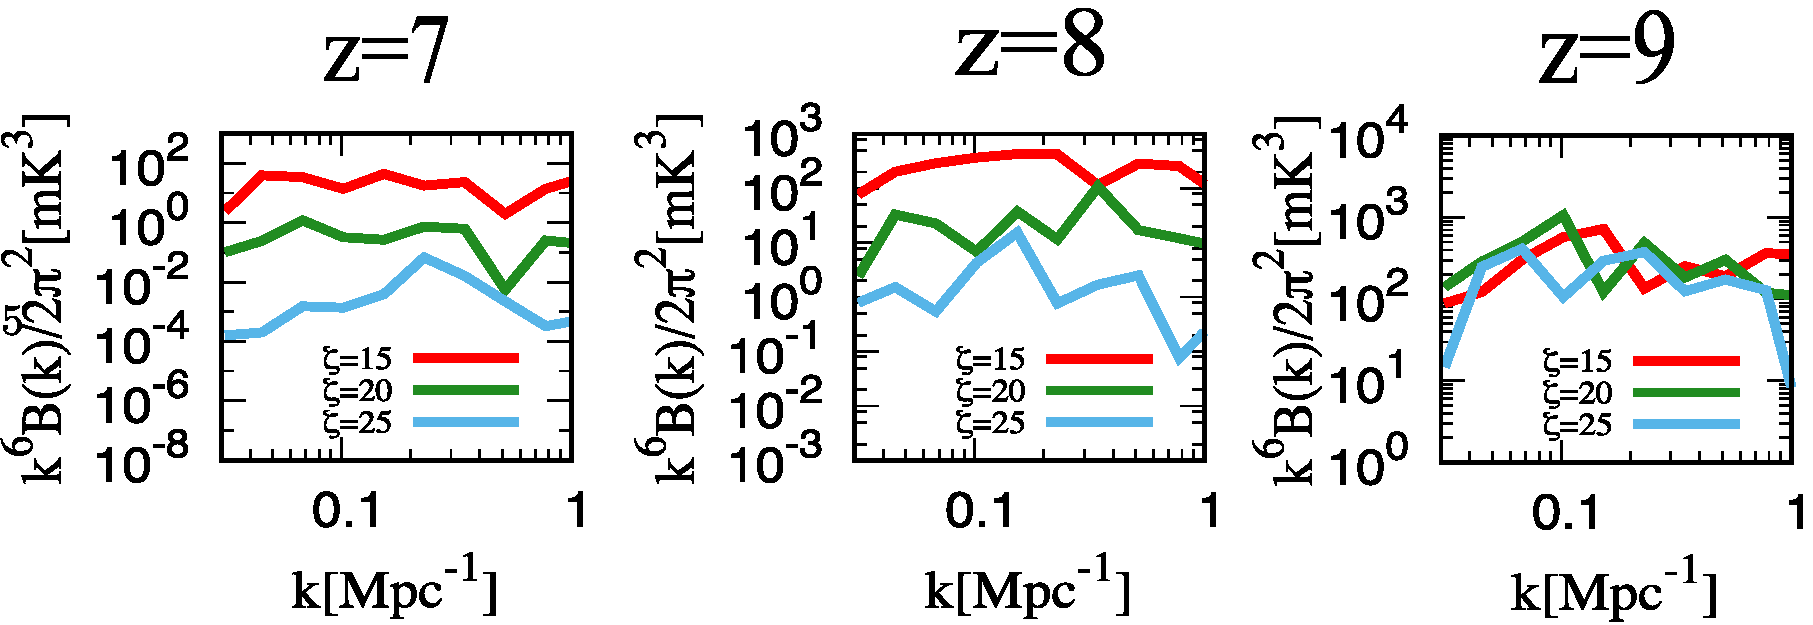
\includegraphics[trim = 0.2cm 1cm 0.2cm 0.2cm, scale = 0.5]{Greig/EqBS}
\end{center}
\caption{Variation in the amplitude of the equilateral bispectrum at $z=7$, 8 and 9 for different ionising efficiencies, $\zeta$, from \cite{Shimabukuro:2017}.}
\label{fig:EqBS}
\end{figure}

Note that the bispectrum is not measured independently from the power spectrum, thus both the power spectrum and bispectrum can be combined to considerably improve our understanding of the underlying astrophysics ({\color{red} can refer to the equivalent case for cosmology where the combination of the two improve the constraining power}).

In recent times, the 21-cm bispectrum has gained considerable traction in interpreting the astrophysics of reionisation and the cosmic dawn. {\color{red} add in citations here works exploring the bispectrum, and quickly what they are exploring}.

Some examples of the exploration of the 21-cm bispectrum. \cite{Watkinson:2019,Watkinson:2017,Shimabukuro:2016}

\subsection{Trispectrum} \label{sec:bispectrum}

I am certain someone looked at the trispectrum...

\subsection{One-point statistics}

Rather that measuring the Fourier transform (e.g. power spectrum) of the 21-cm brightness temperature signal, $\delta_{21}(\mathbf{x})$, we can instead measure the one-point statistics (or moments) of the probability distribution function (PDF). In fact, we have already discussed the lowest order one-point statistic, that is, the mean of $\delta T_{b}(\mathbf{x})$ given by the global signal (see \ref{sec:global}).  These one-point statistics of the PDF essentially measure the deviations away from a fully Gaussian PDF, thus they are by definition sensitive to the non-Gaussian nature of the 21-cm signal. Generally speaking, the one-point statistics of $\delta T_{b}(\mathbf{x})$ are given by,
\begin{eqnarray}
m_{n} = \frac{1}{N}\sum^{N}_{i=0}(\delta T_{b}(\mathbf{x_{i}}) - \bar{\delta T_{b}})^{n},
\end{eqnarray}
where $m_{n}$ is the $n$-th order moment and $N$ is the number of pixels over which the signal is measured. For the 21-cm signal, these moments would be generated from the observed two-dimensional tomographic maps of the 21-cm signal.

The next lowest order statistic of the PDF following the mean is the variance, $\sigma^{2}$. The variance is equivalent to the average of the power spectrum over all Fourier modes, $k$,
\begin{eqnarray}
\sigma^{2} = (\bar{\delta T_{b}})^{2} \int \frac{d^{3}k}{(2\pi)^{3}} P(\mathbf{k}).
\end{eqnarray}
As it is the average over all spatial information, the variance itself is less sensitive to the underlying astrophysics than the power spectrum. However, the strength of one-point statistics shines through when using the higher order moments in combination with the variance (or power spectrum). The next two higher order moments are referred to as the skewness and the kurtosis. Equivalent to the variance's relation to the power spectrum, the skewness and kurtosis are the average over all Fourier modes of the bispectrum and trispectrum respectively (the three and four-point correlation functions). As such, whereas the power spectrum only measures the 2-point correlations, the skewness and kurtosis reveals insights from the non-Gaussian properties of the 21-cm signal.

\begin{figure}[]
\begin{center}
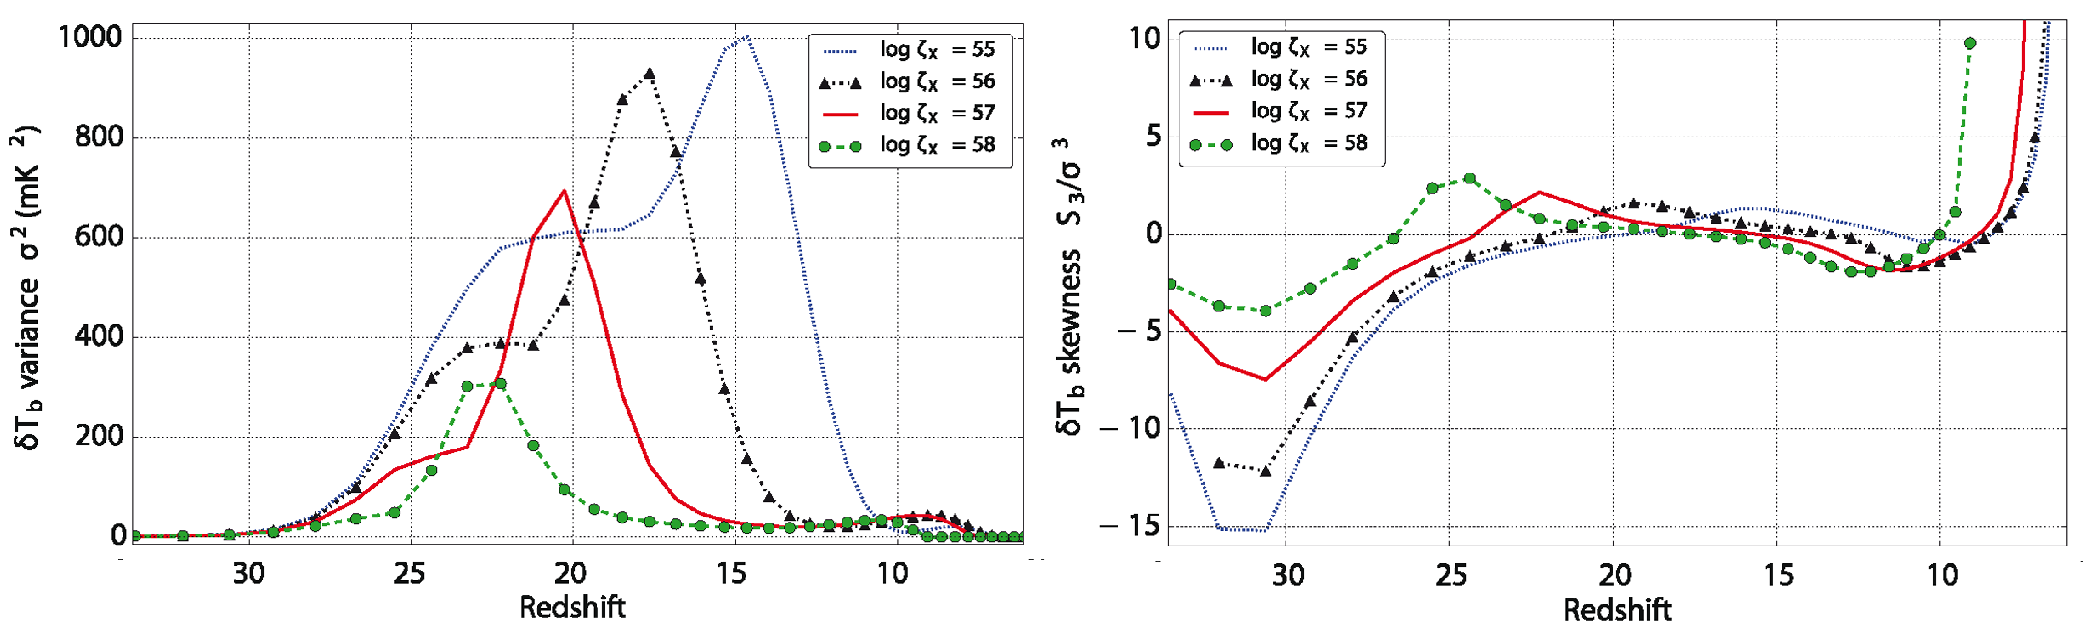
\includegraphics[trim = 0.2cm 1cm 0.2cm 0.2cm, scale = 0.45]{Greig/Skewness}
\end{center}
\caption{The variance (left) and normalised skewness (right) of the 21-cm brightness temperature when varying the efficiency of X-ray heating in the IGM from \cite{Watkinson:2015}.}
\label{fig:skewness}
\end{figure}

The amplitude of the variance is sensitive to differences in the 21-cm brightness temperature. For example, during the EoR, as the number of ionised regions increases (i.e. the contrast between the 21-cm signal from the neutral regions compared to zero signal from the ionised regions) the variance increases. It subsequently turns over as most of the volume is ionised. The skewness is a measure of the asymmetry of the underlying PDF. A negative skewness corresponds to a longer tail towards a lower amplitude signal and a positive skewness corresponds to a longer tail towards higher amplitude signals. The kurtosis is essentially a measure of the outliers of the distribution, with increasing positive (negative) kurtosis corresponding to larger positive (negative) amplitude outliers.

Figure~\ref{fig:skewness} shows an example of both the variance (left) and normalised skewness (right panel) of the 21-cm brightness temperature under different levels of X-ray heating. For increasing X-ray efficiencies (i.e. increase heating) the peak of the variance decreases in amplitude while shifting to earlier times. Increasing the efficiency allows the X-ray heating to occur earlier, reducing the contrast between the $T_{\rm CMB}/T_{\rm S}$ resulting in a lower amplitude peak in the variance. This same behaviour equally results in larger skewness for decreasing X-ray efficiency, owing to a more asymmetric PDF of 21-cm brightness temperatures due to the increasing contrast in $T_{\rm CMB}/T_{\rm S}$. Clearly from Figure~\ref{fig:skewness} it can be seen that these one-point statistics are capable of distinguishing between different astrophysical models.

{\color{red} Some (but not all) references for the one-point statistics. \cite{Harker:2009,Patil:2014,Kittiwisit:2016,Kubota:2016,Watkinson:2014,Shimabukuro:2015,Ross:2017}}

\subsection{Wavelets}

Thus far we have only considered either real-space quantities such as the one-point statistics or the Fourier transform of the $n$-point correlation functions (i.e. the power spectrum and bispectrum). The Fourier transform measures the amplitude of the fluctuations of a given spatial scale, and in order to increase the signal-to-noise we must average the signal over all line-of-sight modes within some observed bandwidth. As a result, we average over modes containing different redshift evolutions and thus increase the bias of the signal. This can be minimised somewhat, for the case of the power spectrum, by averaging the signal over relatively narrow observing bandwidths. However, it still results in some loss in fidelity of the signal.

Instead, in \cite{Trott:2016} the authors explore the potential usage of wavelets, which provide multiple alternatives to the Fourier basis set. Specifically, they explored the application of the Morlet Transform. This provides a family of curves which provide the ability to localise the 21-cm signal both spatially and in frequency. In doing so, the equivalent to the power spectrum, the Morlet power spectrum is capable of providing an unbiased estimator which maximises the three dimensional nature of the 21-cm signal. Preliminary analysis shows that the Morlet power spectrum performs more optimally than the Fourier power spectrum. A physical interpretation of the Morlet power spectrum in the context of the evolution of the 21-cm signal has yet to be explored.

\subsection{Topological measurements of the 21-cm signal}

All previous approaches discussed up till this point have characterised the 21-cm signal using some form of statistical analysis, on the basis of maximising the signal-to-noise. However, the most advanced radio interferometers ({\color{red} do I need to name them or refer to future chapter?}) should enable two dimensional images of the 21-cm signal. These images will contain the complicated morphology of the hot/cold patches of the 21-cm brightness temperature throughout the history of reionisation and the cosmic dawn. The relative sizes, shapes and clustering of these hot/cold patches can reveal numerous insights into the underlying astrophysical processes, such as the number density of sources, their contribution to the heating/ionisation of the IGM and the shape of the emitted spectrum of radiation. The study of these geometric shapes in mathematics is referred to as topology.

Topological studies of reionisation and the cosmic dawn are complimentary to the statistical methods described above. For example, reionisation proceeds through three main stages (e.g. \cite{Gnedin:2000,Furlanetto:2016}): pre-overlap, over-lap and post-overlap. In pre-overlap, the first ionised H {\scriptsize II} regions (or bubbles) grow completely in isolation roughly until $x_{\rm HI} \geq 0.1$. Over-lap ($ 0.9 \geq x_{\rm HI} \geq 0.1$) describes the merging of these ionised bubbles into essentially a single large connected ionised region. Finally, post-overlap $x_{\rm HI} \geq 0.9$ corresponds to the breaking down of the last remaining patches of neutral IGM into smaller and smaller islands. Topological studies are capable of breaking down these transitions by describing the ratios of ionised and neutral regions, how the ionised (or neutral) regions are connected together and how they are embedded in the larger structures as they form. This provides unique insights into the reionisation epoch not available from statistical methods.

There are numerous methods to attempt to characterise the topology of the 21-cm signal. Below, we summarise several of the main approaches taken in the literature. Fundamental to topological studies is the definition of how to identify regions of interest. Typically, a threshold value is required, with the quantity above/below this threshold being used to distinguish the two regions.

\subsubsection{Genus or the Euler characteristic}

The genus, $g$, is a topological property that defines the number of cuts one can make to an object (i.e. H {\scriptsize II} region) without dividing it into independent disconnected sub-regions. It can simply be expressed as,
\begin{eqnarray}
g = N_{\rm >th} - N_{\rm < th}
\end{eqnarray}
where $N_{\rm >th}$ and $N_{\rm < th}$ are the number of connected (or fully enclosed) regions above and below the threshold value for identification. By gradually increasing the threshold value from some initial starting value, a genus curve is constructed, which is a measure of the connectedness of the quantity as a function of different threshold values (e.g. $x_{H {\rm \scriptsize I}}$, $\delta T_{b}$). Typically, these threshold values are expressed in units of the standard deviation from the mean.

The genus has been explored, both in two and three dimensions, either in the context of the ionised (or neutral) field (\cite{Gleser:2006,Lee:2008,Friedrich:2011}) or the 21-cm brightness temperature field (\cite{Hong:2014,Wang:2015}). However, it has yet to be explored in the context of the heating epoch (i.e. $T_{\rm S} \gg T_{\rm CMB}$ is typically assumed). For a purely Gaussian field, the genus curve is symmetric around zero. Thus deviations from symmetry highlight the non-Gaussianity of the 21-cm signal. 

Differences in the evolution in the amplitude of the genus as a function of threshold density can distinguish different source biases and ionising efficiencies. For example, reionisation driven by larger, more biased sources exhibits a different topology than one driven by numerous fainter sources. This appears as changes in the amplitude of the genus as a function of threshold. When the ionised regions are isolated, the genus amplitude is higher than when they begin to overlap (as the total number of isolated ionised regions decreases).

\subsubsection{Minkowski functionals}

A more generalised description of the geometry or topology of the 21-cm signal can be obtained from what are referred to as Minkowski functionals. These are well known concepts from the branch of mathematics known as integral geometry. Three dimensional space is completely defined by four Minkowski functionals. Used heavily in cosmology, in particular large-scale structure {\color{red} need to add citations?}, recently they have gained favour for describing the topology of reionisation \cite{Gleser:2006,Friedrich:2011,Yoshiura:2017,Chen:2018}.

For a zero mean scaler function, $u(x)$, (e.g. $\delta T_{\rm b}$) within a volume, $V$, and standard deviation, $u$, we can define an excursion set, $F_{\nu}$, which contains all points that satisfy the threshold, $u(x) \geq \nu\sigma$, where $\nu = u_{\rm th}/\sigma$ and $u_{\rm th}$ is the threshold value. Mathematically, this gives rise to the following Minkowski functionals,
\begin{eqnarray}
V_{0}(\nu) = \frac{1}{V}\int_{V} {\rm d^3}x\,\Theta\left[u(x) - \nu \sigma\right] \\
V_{1}(\nu) = \frac{1}{6V}\int_{\partial F_{\nu}} {\rm d}s \\
V_{2}(\nu) = \frac{1}{6\pi V}\int_{\partial F_{\nu}} {\rm d}s\,\left[\kappa_{1}(x) + \kappa_{2}(x)\right] \\
V_{3}(\nu) = \frac{1}{4\pi V}\int_{\partial F_{\nu}} {\rm d}s\, \kappa_{1}(x)\kappa_{2}(x).
\end{eqnarray}
Here, $\Theta$ is the Heaviside step-function, $\partial F_{\nu}$ is the surface of the excursion set, ${\rm d}s$ is the surface element and $\kappa_{1}(x)$ and  $\kappa_{2}(x)$ are the principle curvatures (inverse of the principle radii) at $x$. The zeroth Minkowski functional, $V_{0}$, corresponds simply to the total volume of the excursion set (i.e. volume above the threshold value), $V_{1}$ and $V_{2}$ correspond to the total surface and mean curvature of the excursion set while $V_{3}$ is the integrated Gaussian curvature over the surface or the Euler characteristic (also $\chi$). The Euler characteristic is related to the genus, $g$, via $V_{3} = 2(1-g)$ thus it effectively describes the shape of the excursion set. Thus, the full set of Minkowski functionals contain additional information beyond that of just the genus.

Generally speaking the following behaviour is expected of the Minkowski functionals throughout reionisation and the cosmic dawn. $V_{0}$ describes the volume contained above/below the threshold value. For example, if $V_{0} \sim 0.5$ at $\delta T_{\rm b} = 0$ this implies the number of hot/cold patches are roughly equal. The $V_{0}$ curve will move from left to right (to increasing $\delta T_{\rm b}$) as heating occurs. $V_{1}$ (reflected in $V_{2}$) exhibits a similar shift to higher $\delta T_{\rm b}$, however it is initially strongly peaked with a high density tail containing the heated regions. This peak smooths out over a broader range of $\delta T_{\rm b}$ as heating continues. During reionisation, $V_{1}$, $V_{2}$ and $V_{3}$ will shift toward $\delta T_{\rm b}=0$ as the higher amplitude $\delta T_{\rm b}$ regions ionise first.  {\color{red} Is this description even relevant without a figure? Don't want to include too many figures...}

\begin{figure}[]
\begin{center}
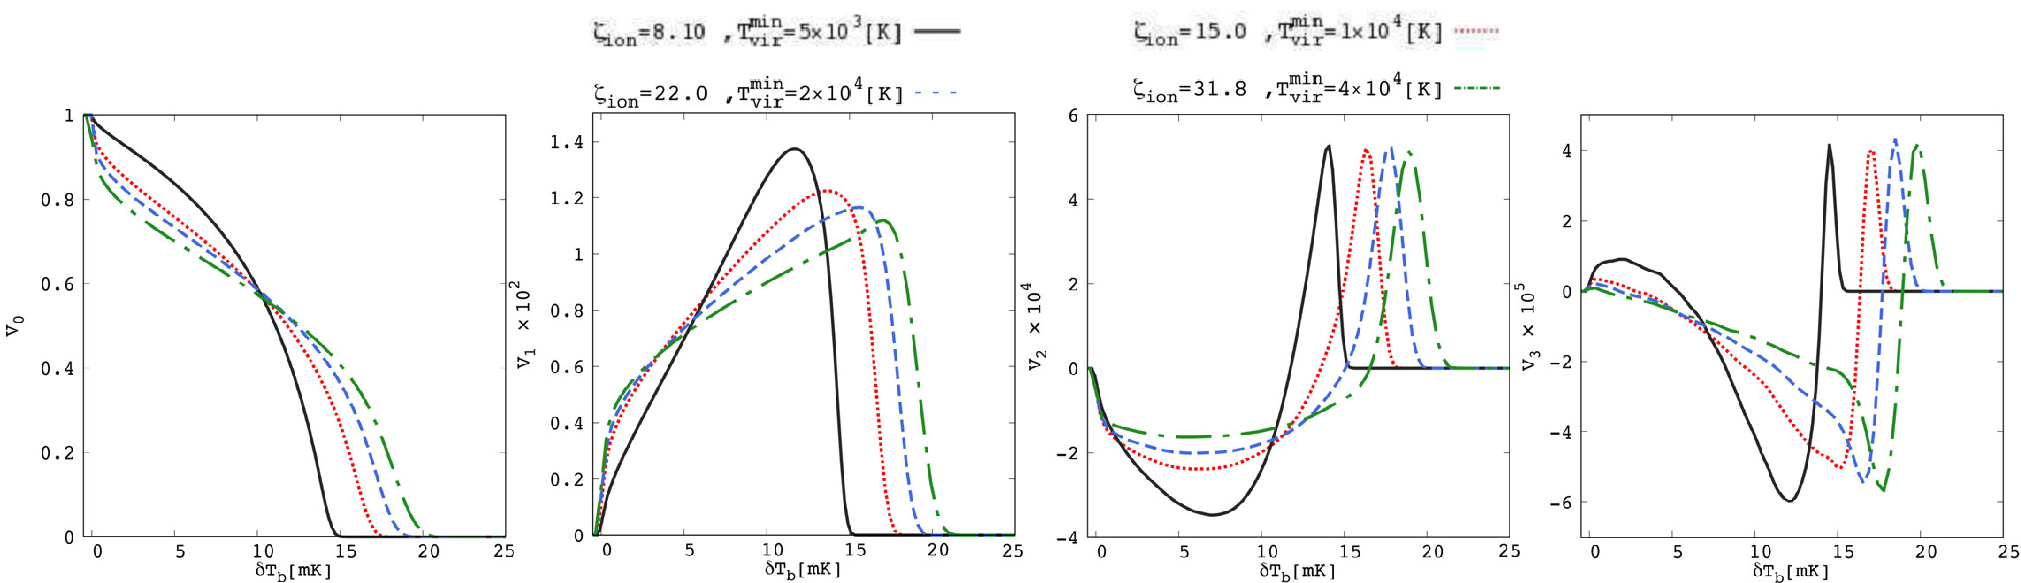
\includegraphics[trim = 0.2cm 1cm 0.2cm 0.2cm, scale = 0.475]{Greig/MFvary}
\end{center}
\caption{The impact of varying the astrophysical parameterisation for a fixed neutral fraction ($x_{H_{\rm \scriptstyle I}}\approx 0.5$) and redshift ($z=8.6$). Consider the impact of varying either the ionising efficiency $\zeta$ or the minimum halo mass for star-forming galaxies, $T_{\rm vir}$ on the four Minkowski functionals. Figure adapted from \cite{Yoshiura:2017}.}
\label{fig:MFs}
\end{figure}

In Figure~\ref{fig:MFs} we show the four Minkowski functionals for the 21-cm brightness temperature when varying the underlying astrophysical processes from \cite{Yoshiura:2017} at a fixed neutral fraction ($x_{H_{\rm \scriptstyle I}}\approx 0.5$) and redshift ($z=8.6$). Here, these authors consider variations in either the ionising efficiency, $\zeta$, or the minimum halo mass hosting star-forming galaxies, $T_{\rm vir}$. Clearly, different reionisation histories are distinguishable by the Minkowski functionals.

\subsubsection{Shape-finders}

An extension to Minkowski functionals, shape-finders ({\color{red} need citations to the method}) are a way to characterise the shapes of compact surfaces. Applied to reionisation (\cite{Bag:2018,Bag:2019}), these shape-finders can provide a means to characterise how the ionised regions grow. For example, they are useful in being able to distinguish between whether the topology is planar or filamentary. Shapefinders are derived directly from the Minkowski functionals via:
\begin{eqnarray}
{\rm Thickness}: T = \frac{3V_{0}}{V_{1}} \\
{\rm Breadth}: B = \frac{V_{1}}{V_{2}} \\
{\rm Length}: L =  \frac{V_{3}}{4\pi}.
\end{eqnarray}
These shape-finders are interpreted as providing the three principle axes of a physical object. The morphology of the ionised region can then be defined by either the planarity or its filamentarity:
\begin{eqnarray}
{\rm Planarity}: P = \frac{B - T}{B + T} \\
{\rm Filamentarity}: F = \frac{L - B}{L+B},
\end{eqnarray}
where $P\gg F$ corresponds to planar objects (i.e. sheets) while the opposite $F\gg P$ corresponds to a filament.

During the reionisation epoch, percolation theory shows that a single infinitely large, multiply connected ionised region will rapidly form ({\color{red} add citations}). When describing the largest singly connected ionised region, \cite{Bag:2018,Bag:2019} find that both $T$ and $B$ evolve slowly whereas $L$ increases rapidly. Thus, this large ionised region grows only along its `length' implying a highly filamentary structure.

\subsubsection{Persistent homology theory}

Homology characterises the topology of the ionisation bubble network into its fundamental components: ionised regions, tunnels (enclosed neutral filaments) and cavities (patches of neutral hydrogen). The persistence then quantifies the significance of the feature, for example its lifetime, by computing a birth and death date for an object.  Thus far, it has only been applied to the ionisation field (\cite{Elbers:2019}). These ionised regions ($\beta_{0}$), tunnels ($\beta_{1}$) and cavities ($\beta_{2}$) can be described by the so-called Betti numbers, which contain the total number of each. These can be related to the earlier Euler characteristic via, $\chi = \beta_{0} - \beta_{1} + \beta_{2}$. By breaking the Euler characteristic into the constituent components and tracking their individual growth reveals additional information on the topology, thus it is a more generalised method than either the genus of the Minkowski functionals.

\subsubsection{Fractal dimensions}

An alternative to classifying the ionised (neutral) regions embedded in the 21-cm signal is through a fractal dimensions analysis. Applied to reionisation (\cite{Bandyopadhyay:2017}), this provides a direct means to quantify the deviation away from a homogenous distribution, as well as the degree of clustering and lacunarity (a measure of the size of the ionised regions). The fractal dimension, $D_{q}$, also known as the Minkowski-Bouligand dimension, is a measure of how complicated the topology of the field in question is. A homogeneous distribution in three dimensions has a $D_{q}=3$. \cite{Bandyopadhyay:2017} show that the topology of reionisation exhibits a significant multi-fractal behaviour. These authors find that the fractal dimension is relatively insensitive to the minimum halo mass of the star-forming galaxies, however it was sensitive to the mass averaged ionisation fraction. Thus, the correlation dimension can be useful for constraining the global neutral fraction. Additionally, it is a strong discriminant of models of outside-in and inside-out reionisation.

\subsubsection{Contour Minkowski tensor}

In \cite{Kapahtia:2018,Kapahtia:2019}, these authors introduced the rank-2 contour Minkowski tensor ({\color{red} add citations}) in two-dimensions which can probe both the length and time scales of the ionised regions during reionisation. The Minkowski tensors are a generalisation of the scalar Minkowski functionals. The contour Minkowski tensor provides information on both the alignment of structures in two dimensions and their anisotropy. Since the ionised regions are not perfectly spherical, their shape anisotropy can be explored by the ratio of the two eigenvalues of the contour Minkowski tensor while the amplitude of the eigenvalues describes their size.

In this analysis, the number of connected regions and holes (e.g. the Betti numbers) given a specific threshold value are tracked. In addition, a characteristic radius of the structures and their shape anisotropy can be determined. For a description of the evolution of $\delta T_{\rm b}$, we refer the reader to \cite{Kapahtia:2019}, ignoring it here owing to its complexity due to the definition of the connected regions and holes as a function of the threshold value as the 21-cm signal transitions transition from hot/cold regions in the heating epoch to neutral/ionised regions during reionisation ({\color{red} would require several figures and long descriptions. Don't think thats required here (hopefully not)}). However, we emphasise that these authors explored varying the minimum mass hosting star-forming haloes and clearly show that different astrophysical parameters can be distinguishable.

\subsection{Bubble size distributions}

Throughout reionisation and the cosmic dawn, the morphology of the 21-cm signal is driven by processes that embed a morphological signature on the 21-cm signal. For example the ionised H$_{\rm \scriptsize II}$ regions or the hot/cold spots in the 21-cm brightness temperature during the heating epoch. Quite simply, if we could measure the distribution of these `bubbles' and how they evolve over cosmic time we would have a strong discriminant of the populations of sources responsible for the heating and ionisation of the IGM and also the spectrum of their emitted radiation. Effectively, this would behave as a statistical distribution function (number of bubbles given a physical scale) analogous to a halo mass function.

However, the bubbles do not remain isolated, very quickly overlapping into increasingly large and topologically complex structures. Thus, there is no unique way to characterise these bubbles. Nevertheless several methods have been explored in order to be able to construct a probabilistic distribution of the bubble sizes.

The simplest approach is to perform a friends-of-friends approach ({\color{red} add citations here}), which simply connects all cells above (below) a threshold value. However, very rapidly a single large ionised structure exists which fills most of the volume with only a small fraction of isolated regions remaining. The relative volume of this large ionised region and the distribution of the smaller regions can still differentiate reionisation morphologies, however there is less statistical weight.

An alternative approach is to place a sphere on every pixel, averaging out the signal across increasingly larger spheres until a radius is found where the average signal is above the threshold value ({\color{red} add citations here}). While this generates a more statistical meaningful distribution of bubbles, these sizes tend to overestimate the size of the topological feature of interest due to the assumed spherical symmetry.

Recently, more statistically robust methods have been introduced to measure the bubble size distributions. First of these is the mean free path method, which uses a Monte Carlo approach by considering a large number of random positions and determining the distance to the edge of the bubble from different random directions ({\color{red}} add citations here). This results in an unbiased estimator of the bubble size distribution. Next, adapted from the cosmological search for voids, the Watershed ({\color{red} add citations here}) method has been explored. This is a well known two-dimensional image segmentation algorithm creating contours of constant value (i.e. $\delta T_{b}$) which are treated as levels of a tomographic map. These are then `flooded' to obtain unique locations for the minima (e.g. ionised regions).

Remaining in the image processing regime, ({\color{red} add citations here}) introduced the superpixels method. This uses a region based method to identify regions of complex shapes (i.e. ionised regions) segmenting these regions into smaller segments called superpixels. The bubble size distribution is then obtained by averaging the value of the 21-cm brightness temperature within each segment ({\color{red} search for specific details on how this becomes a bubble distribution}).

Granulometry


\subsection{Individual bubbles}

Images will provide a direct tangible link to the process of reionisation. Revealing exactly where ionising bubbles are, and thus where to look for the sources responsible for the bubble creation. 

However, bubble identification will become rather problematic, as it is the differential brightness that is observed, not the raw brightness temperature. Need smart/sophisticated approaches to search and characterise the signal.

Look at individual regions of interest, i.e. around a bright QSO or large number of galaxies. 

Matched filters etc., are useful for finding/detecting isolated bubbles

\subsection{Stacked images}

May be difficult to detect individual objects, instead, one could stack 21cm spectra centred on known galaxies. See Paul Geil's paper.

Border's on potential discussions of synergies. Requires known locations of ionising sources with precise redshifts and positions of the sky. JWST/WFIRST. Is there 

\subsection{Other statistics}

Are there other statistics that I have overlooked/forgotten. Need to do a search of the literature to ensure I have covered everything.

\section{Efficient methods to model/simulate the 21cm signal}

Ideally we want to use the largest, most physically accurate simulations to match the observed 21cm signal. However, this is not practical. Instead, we must come up with methods to compensate accuracy for efficiency.\\
\\
Originally I envisaged this section to go as follows
\begin{itemize}
\item Discuss briefly that numerical simulations are great but too computationally expensive
\item Highlight semi-numerical/analytic simulations as fitting the bill by being faster etc.
\item Then discuss alternatives (i.e. emulators).
\end{itemize}
This will need to be re-worked given Jordan's plan to discuss this. I haven't yet thought of a logical plan to motivate this. I guess one way would be to concatenate it into just a simulation section and briefly summarise what was discussed in Jordan's chapter (which is a couple of chapters ago, so might be appropriate to do so). It's less obvious to move into discussing emulators in the absence of motivating the need for them by highlighting the complications of simulations in general.

\subsection{Numerical simulations}

Ideally, use large, numerical simulations to make a realisation which matches observation. Want to include as much physics as possible into these simulations. Doing so, comes at a serious cost. Simulating the 21cm signal is complicated! Brief summary on the required dynamic range. Briefly highlight the expensive nature of these simulations, Hydrodynamics, radiative transfer etc. Quickly becomes computationally prohibitive to run more than a couple of realisations. \textbf{Jordan's section (Modelling Tools) will likely cover most if not all of this}.

\subsection{Semi-numerical/analytic models of the 21cm signal}

Enter semi-numerical approaches, which broadly encapsulate the global average quantities of reionisation and the cosmic dawn and reproduce morphologically similar realisations of the 3D structure. The advantage here is that the computational costs are drastically reduced (orders of magnitude less). \textbf{Jordan's section (Modelling Tools) will likely cover most if not all of this}.

\subsection{Intelligent sampling of the parameter space}

Running simulations to span all of the allowed parameter space may be too computationally intensive. However, perhaps we can make intelligent assumptions/guesses about how many simulations to run, and on a specific area of physics to focus on. Some of the concepts here may overlap slightly with the Emulator section below. This sampling was discussed in one of Benoit's recent papers.

\subsection{Emulators}

An alternative to directly running a simulation to estimate some astrophysical statistic/model, one can instead construct a function which estimates what the statistical signal should be, given some astrophysical or cosmological parameter set. This is what is referred to as an emulator. Using simulations, a generator function is constructed which can approximate the statistics of the signal. Results in multiple orders of magnitude improvement in computational speed as no new simulations are required. However, it can only approximate statistics, it does not generate 3D simulations. 

Developing an emulator benefits from efficient parameter space approaches, as it minimises the size of the database required to construct the emulator. There are a variety of approaches to consider when attempting to minimise the sampling of the astrophysical parameter space. For example Latine-Hypercube, Gaussian processes... Can briefly discuss each method, and a few recent papers that explore methods to do this

There are numerous machine learning approaches to construct an emulator.

Discuss Nick Kern's of 21cmFAST and Cohen's global signal one of Anastasia's code.

Highlight and discuss Chardin et al. (2019). Emulation of reionisation simulations (construction of treion maps given source lists). arxiv:1905.06958

\subsection{Characterising our ignorance}

We are fully aware that semi-numerical approaches are inaccurate at 10s of per cent level. Additionally, they oversimplify/completely ignore the underlying astrophysical properties. However, if the global quantities (observables such as luminosity functions etc.) can still be reproduced within agreement, we can develop an understanding of how one might map from a semi-numerical simulation, to a more realistic simulation. Basically, tell the large, computationally expensive simulation where exactly to look in the region of parameter space.

Using summary statistics and globally average observables, we can develop a means to calibrate one simulation to mimic the outputs of another. In other words, develop a bias or functional form to smooth out uncertainties from one simulation to mimic the results of a more detailed simulation.

Describe ongoing attempts to quantify this. i.e. use luminosity functions to calibrate simulations, apply redshift corrections to deal with photon non-conservation etc.

These correction factors etc., will be crucial for inferring astrophysics and cosmology from the 21cm signal


\section{Inference methods for 21cm}

Having discussed methods to model/simulate the 21cm signal, now need to shift focus to methods to infer information about the astrophysics/cosmology from the 21cm signal.

\subsection{Fisher Matrices}

Simplest method, which takes derivatives with respect to model parameters of a functional form (i.e. a 21cm statistical signal) to infer parameter constraints. Effectively, exploits how sensitive the 21cm signal is to specific parameters. Limiting assumption include Gaussianity etc.

Successfully used for cosmology

\subsection{Bayesian MCMC}

Significantly more robust method to parameter inference. Outline Bayes' theorem. Highlight that this basically boils down to exploring by random walks, using a likelihood function and priors to accept/penalise regions of parameter space. Very useful for recovering constraints. Again, successfully used in Cosmology etc.

Describe its use in the context of 21cm. Introduce 21CMMC, and a couple of other codes that use MCMC (Sultan's simfast21, Jordan's global signal, Geraint's MCMC, Simon's Mhysa). Highlight that 21CMMC is the only direct MCMC. Emphasise that techniques such as emulators can be coupled with MCMC to improve overall computational efficiency at the cost of some further inaccuracies.

Don't forget the Bernardi and Zwart papers.

\subsection{Nested sampling and model inference}

We have a wide variety of simulations, each with their own strength's and weaknesses. In principle, various models/simulations/physical prescriptions can be discriminated against using model selection or inference. Related to MCMC, nested sampling can focus on model selection rather than simply astrophysical recovery. Can refer to Tom Binnie's recent paper.

\subsection{Neural Networks}

Instead of using MCMC to recover parameters from statistics, we can use the full 2/3D images of the 21cm signal with neural networks. One can construct a database of simulations and extract the 21cm signal to construct a neural network. This network can then learn an large number of properties, i.e. how changes in the topology are affected by astrophysical parameters etc. Using this technique one can directly convert from an observed 2D image to the underlying astrophysics. Like emulators, the application of the network is extremely quick. Downsides are parameter errors etc. and in some sense physical intuition. It tells you an answer, but not why.

Simulated images of the 21cm signal have already been used to infer astrophysical and cosmological constraints. For example with convolutional networks (e.g Nicolas or Paul La Plante). Discuss other machine learning approaches.



\iffalse

Lorem ipsum dolor sit amet, consectetur adipiscing elit. Duis eu egestas erat. Maecenas tincidunt lacinia tincidunt. Mauris id lectus nec neque feugiat condimentum vitae at diam. In vel orci nunc, non commodo mauris. Vivamus ipsum enim, vulputate quis pharetra non, molestie quis felis. Vivamus porttitor placerat turpis at accumsan. Nunc tortor velit, faucibus a rhoncus nec, blandit non elit. Nam consectetur lectus eu nisi blandit dapibus rhoncus dui tempus. Mauris fermentum dolor vel ipsum vulputate sit amet ultricies tortor lacinia. Donec ut nibh erat. Morbi nec mi ante. Integer nec vestibulum diam. Donec tincidunt pellentesque quam, ut interdum mauris venenatis condimentum. Nam condimentum, augue in aliquet gravida, neque dui elementum eros, id semper eros purus sed felis. Curabitur in justo sit amet sapien ultrices hendrerit at quis nibh. Quisque iaculis pulvinar tincidunt. 
\begin{eqnarray}
C(12) &= &\left[\overrightarrow{\pi}\cdot\overrightarrow{\phi}(x+r)\right] \nonumber \\ 
&\approx& 1-\mathrm{const}\frac{r^2}{L^2}\int_r^L\frac{x\rmd x}{x^2} + \cdots \nonumber  \\
&\approx& 1-\mathrm{const}\frac{r^2}{L^2}\ln\frac{x\rmd x}{x^2} + \cdots .\label{brokenlongeqn}
\end{eqnarray}

Aenean tellus risus, porta sit amet porta vitae, tincidunt ut felis. Class aptent taciti sociosqu ad litora torquent per conubia nostra, per inceptos himenaeos. Vestibulum ante ipsum primis in faucibus orci luctus et ultrices posuere cubilia Curae; Phasellus pulvinar placerat velit auctor egestas. Vivamus euismod fringilla tincidunt. Sed ut magna felis, id sollicitudin nunc. Quisque a dui eu erat consectetur egestas a quis justo. Aenean euismod congue diam, vel posuere urna fermentum sit amet. Lorem ipsum dolor sit amet, consectetur adipiscing elit. Mauris faucibus lacus eget est mollis auctor. Donec at nibh ligula, et posuere massa. Phasellus quis leo diam \cite{diamantaras1996pcn}.
Donec aliquam blandit risus, eu venenatis ante euismod eu. Curabitur cursus justo id arcu condimentum feugiat. Integer sapien urna, vulputate et adipiscing nec, convallis et justo. Suspendisse in ipsum at felis ornare interdum \cite{tulone2006pts},

\begin{figure}[]
\begin{center}

\includegraphics[width=0.5\textwidth]{Greig/01x01-eps-converted-to}
\end{center}
\caption{This is figure 1 in chapter 1.}
\end{figure}

\paragraph{Cras adipiscing} sagittis nunc vel luctus. Suspendisse volutpat augue quis erat semper consequat dignissim tellus euismod. Morbi hendrerit, tellus id aliquam iaculis, nibh leo tincidunt eros, vitae varius ligula felis in mi.

\begin{table}
\caption{Greek Letters.}
\begin{center}
\begin{tabular}{llllllll}
\hline
$\alpha $  & $ \beta $  & $ \gamma $  & $ \delta $  & $ \epsilon $  & $ \varepsilon $  & $ \zeta $  & $ \eta $ \\
 $ \theta $  &  $ \vartheta $  &  $ \gamma $  &  $ \kappa $  &  $ \lambda $  &  $ \mu $  &  $ \nu $  &  $ \xi $ \\
 $ o $  &  $ \pi $  &  $ \varpi $  &  $ \rho $  &  $ \varrho $  &  $ \sigma $  &  $ \varsigma $  &  $$ \\
 $ \tau $  &  $ \upsilon $  &  $ \phi$ &  $ \varphi $  &  $ \chi $  &  $ \psi $  &  $ \omega$  &  $ $ \\
 &  &  &  &  &  &  & \\
$ \Gamma $  & $ \Delta $  & $ \Theta $  &  $ \Lambda $  &  $ \Xi $  &  $ \Pi $  &  $ \Sigma $  & $ \Upsilon $ \\
 $ \Phi$ &  $ \Psi $  &  $ \Omega $  &  &  &  &  &\\
\hline
\end{tabular}
\end{center}\end{table}

\begin{figure}[]
\begin{center}

\includegraphics[width=0.6\textwidth]{Greig/01x02}
\end{center}
\caption{This is figure 2 in chapter 1.}
\end{figure}

\fi

\bibliographystyle{plain}
\bibliography{Greig/References}



\chapter{Chapter title}

\begin{bf}
  \author{Author Name}\\
  
Abstract\\
\end{bf}

This chapter discusses some important things


\section{A Section}

Lorem ipsum dolor sit amet, consectetur adipiscing elit. Duis eu egestas erat. Maecenas tincidunt lacinia tincidunt. Mauris id lectus nec neque feugiat condimentum vitae at diam. In vel orci nunc, non commodo mauris. Vivamus ipsum enim, vulputate quis pharetra non, molestie quis felis. Vivamus porttitor placerat turpis at accumsan. Nunc tortor velit, faucibus a rhoncus nec, blandit non elit. Nam consectetur lectus eu nisi blandit dapibus rhoncus dui tempus. Mauris fermentum dolor vel ipsum vulputate sit amet ultricies tortor lacinia. Donec ut nibh erat. Morbi nec mi ante. Integer nec vestibulum diam. Donec tincidunt pellentesque quam, ut interdum mauris venenatis condimentum. Nam condimentum, augue in aliquet gravida, neque dui elementum eros, id semper eros purus sed felis. Curabitur in justo sit amet sapien ultrices hendrerit at quis nibh. Quisque iaculis pulvinar tincidunt. 
\begin{eqnarray}
C(12) &= &\left[\overrightarrow{\pi}\cdot\overrightarrow{\phi}(x+r)\right] \nonumber \\ 
&\approx& 1-\mathrm{const}\frac{r^2}{L^2}\int_r^L\frac{x\rmd x}{x^2} + \cdots \nonumber  \\
&\approx& 1-\mathrm{const}\frac{r^2}{L^2}\ln\frac{x\rmd x}{x^2} + \cdots .\label{brokenlongeqn}
\end{eqnarray}

Aenean tellus risus, porta sit amet porta vitae, tincidunt ut felis. Class aptent taciti sociosqu ad litora torquent per conubia nostra, per inceptos himenaeos. Vestibulum ante ipsum primis in faucibus orci luctus et ultrices posuere cubilia Curae; Phasellus pulvinar placerat velit auctor egestas. Vivamus euismod fringilla tincidunt. Sed ut magna felis, id sollicitudin nunc. Quisque a dui eu erat consectetur egestas a quis justo. Aenean euismod congue diam, vel posuere urna fermentum sit amet. Lorem ipsum dolor sit amet, consectetur adipiscing elit. Mauris faucibus lacus eget est mollis auctor. Donec at nibh ligula, et posuere massa. Phasellus quis leo diam \cite{diamantaras1996pcn}.
Donec aliquam blandit risus, eu venenatis ante euismod eu. Curabitur cursus justo id arcu condimentum feugiat. Integer sapien urna, vulputate et adipiscing nec, convallis et justo. Suspendisse in ipsum at felis ornare interdum \cite{tulone2006pts},

\begin{figure}[]
\begin{center}

\includegraphics[width=0.5\textwidth]{Bernardi/01x01-eps-converted-to}
\end{center}
\caption{This is figure 1 in chapter 1.}
\end{figure}

\paragraph{Cras adipiscing} sagittis nunc vel luctus. Suspendisse volutpat augue quis erat semper consequat dignissim tellus euismod. Morbi hendrerit, tellus id aliquam iaculis, nibh leo tincidunt eros, vitae varius ligula felis in mi.

\begin{table}
\caption{Greek Letters.}
\begin{center}
\begin{tabular}{llllllll}
\hline
$\alpha $  & $ \beta $  & $ \gamma $  & $ \delta $  & $ \epsilon $  & $ \varepsilon $  & $ \zeta $  & $ \eta $ \\
 $ \theta $  &  $ \vartheta $  &  $ \gamma $  &  $ \kappa $  &  $ \lambda $  &  $ \mu $  &  $ \nu $  &  $ \xi $ \\
 $ o $  &  $ \pi $  &  $ \varpi $  &  $ \rho $  &  $ \varrho $  &  $ \sigma $  &  $ \varsigma $  &  $$ \\
 $ \tau $  &  $ \upsilon $  &  $ \phi$ &  $ \varphi $  &  $ \chi $  &  $ \psi $  &  $ \omega$  &  $ $ \\
 &  &  &  &  &  &  & \\
$ \Gamma $  & $ \Delta $  & $ \Theta $  &  $ \Lambda $  &  $ \Xi $  &  $ \Pi $  &  $ \Sigma $  & $ \Upsilon $ \\
 $ \Phi$ &  $ \Psi $  &  $ \Omega $  &  &  &  &  &\\
\hline
\end{tabular}
\end{center}\end{table}

\begin{figure}[]
\begin{center}

\includegraphics[width=0.6\textwidth]{Bernardi/01x02}
\end{center}
\caption{This is figure 2 in chapter 1.}
\end{figure}


\bibliographystyle{plain}
\bibliography{Bernardi/References}



\chapter{Foregrounds and their mitigation}
\begin{bf}
	\author{Emma Chapman (Imperial College London) \\and Vibor Jeli\'c (Ru{\dj}er Bo\v{s}kovi\'c Institute)}\\

	Abstract\\
The low-frequency radio sky is dominated by the diffuse synchrotron emission of our Galaxy and extragalactic radio sources related to Active Galactic Nuclei and star-forming galaxies. This foreground emission  is much brighter than the cosmological 21~cm emission from the Cosmic Dawn and Epoch of Reionization. Studying the physical properties of the foregrounds is therefore of fundamental importance for their mitigation in the cosmological 21~cm experiments. This chapter gives a comprehensive overview of the foregrounds and our current state-of-the-art knowledge about their mitigation.
\end{bf}

\section{What are the foregrounds?}
A detection of the redshifted 21~cm emission from the Cosmic Dawn (CD) and Epoch of Reionization (EoR) is a daunting task due to a number of challenges, which are different in nature and complexity. One of them is the extremely prominent foreground emission, which dominates the sky at low radio frequencies.  This emission intervenes like fog on an autumn morning and obscures our view towards the neutral hydrogen regions from the times of the first ``stars'' in the Universe. To clear the view and to make the detection possible, we need to study the foreground emission in great detail and acquire knowledge about its properties.

The foreground emission can be dived in two main categories: (i) Galactic foregrounds, mostly associated with the diffuse synchrotron and to some extent free-free emission from the Milky Way; and (ii) extragalactic foregrounds, associated with the radio emission from star-forming galaxies and Active Galactic Nuclei, and less relevant radio halos and relics. For an illustration of different foreground components see Fig.~\ref{fig:fgcube}. The former component dominates at angular scales larger than a degree and its contribution to the total foreground power is estimated to about 70\% at 150~MHz \cite{shaver99}. The later component dominates at small angular scales and its contribution is estimated to about 30\% \cite{shaver99}.  Both components are expected to be spectrally smooth due to the dominant synchrotron nature of their emission. 

In comparison to the cosmological 21~cm signal, the foreground emission is three to four orders of magnitudes brighter in total power. This mounts to two to three orders of magnitudes in fluctuations. Thus, the global redshifted 21~cm experiments, which use a single antenna for the measurement (e.g. EDGES, PAPER), need to deal with an order of magnitude brighter foreground emission than the ones using interferometers (e.g. LOFAR and MWA). 

\begin{figure}[!t]
   \centering
    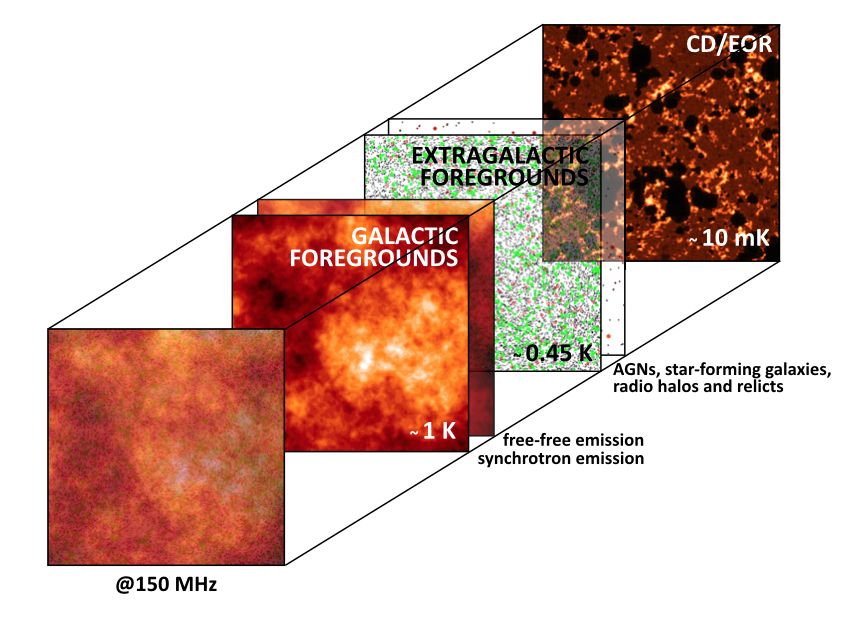
\includegraphics[width=0.95\textwidth]{Chapman_Jelic/Images/fgcube.png}
    \caption{An illustration of different foreground components in the redshifted 21~cm experiments. The images are based on \cite{jelic08, jelic10} simulations of the foreground emission and 21cmFAST simulations \cite{mesinger11}.}
    \label{fig:fgcube}
\end{figure}

Various authors studied the foregrounds in the context of the cosmological 21~cm measurements \cite{shaver99, dimatteo02, dimatteo04, oh03, cooray04, jelic08, deoliveiracosta08, bowman09, jelic10}. These studies mainly used simulations based on statistical properties of the foregrounds extrapolated from the higher radio frequencies.  \cite{shaver99} have given the first overview of the foreground components, while \cite{jelic08} carried the first comprehensive simulation of the foregrounds. This simulation is used extensively in development of the robust foreground mitigation techniques for the LOFAR-EoR project \cite{jelic08,Harker2009MNRAS.393.1449H, Harker2009MNRAS.397.1138H, Harker2010MNRAS.405.2492H, Chapman2012MNRAS.423.2518C, Chapman2013MNRAS.429..165C} and more recently for the SKA CD/EoR project \cite{Chapman2015aska.confE...5C, Chapman2016MNRAS.458.2928C}.  In addition, there are  more complex simulations of both Galactic and extragalactic emission, tailored for studies of the interstellar medium and magnetic fields in the Milky Way \cite{waelkens09,sun09,haverkorn19} or of different populations of the radio sources at low-radio frequencies \cite{wilman08,wilman10,bonaldi19}. These simulations can be also used as the foreground template in the cosmological 21~cm studies.

The first extensive observational study of the foregrounds at low-radio frequencies was conducted by \cite{bernardi09, bernardi10} using the WSRT radio telescope. Three different fields were observed and Galactic emission was constrained both at low and high Galactic latitudes. Once the new low-frequency instruments came online (e.g. LOFAR and MWA), our knowledge of the foregrounds started to grow extensively. In the following sections a more comprehensive overview of the foregrounds is given both in total intensity and polarisation. 

\subsection{Galactic foregrounds in total intensity}
Galactic diffuse synchrotron emission is a dominant foreground component from a few tens of MHz to a few tens of GHz. It is non-thermal in its nature, produced mostly by the relativistic cosmic-ray electrons and to some extent positrons that spiral around the interstellar magnetic field lines and emit radiation.  Above a few tens of GHz free--free emission from diffuse ionized gas and thermal dust emission start to dominate over the synchrotron emission (see Fig.~\ref{fig:galcomp}). 

\begin{figure}[!t]
\centering
    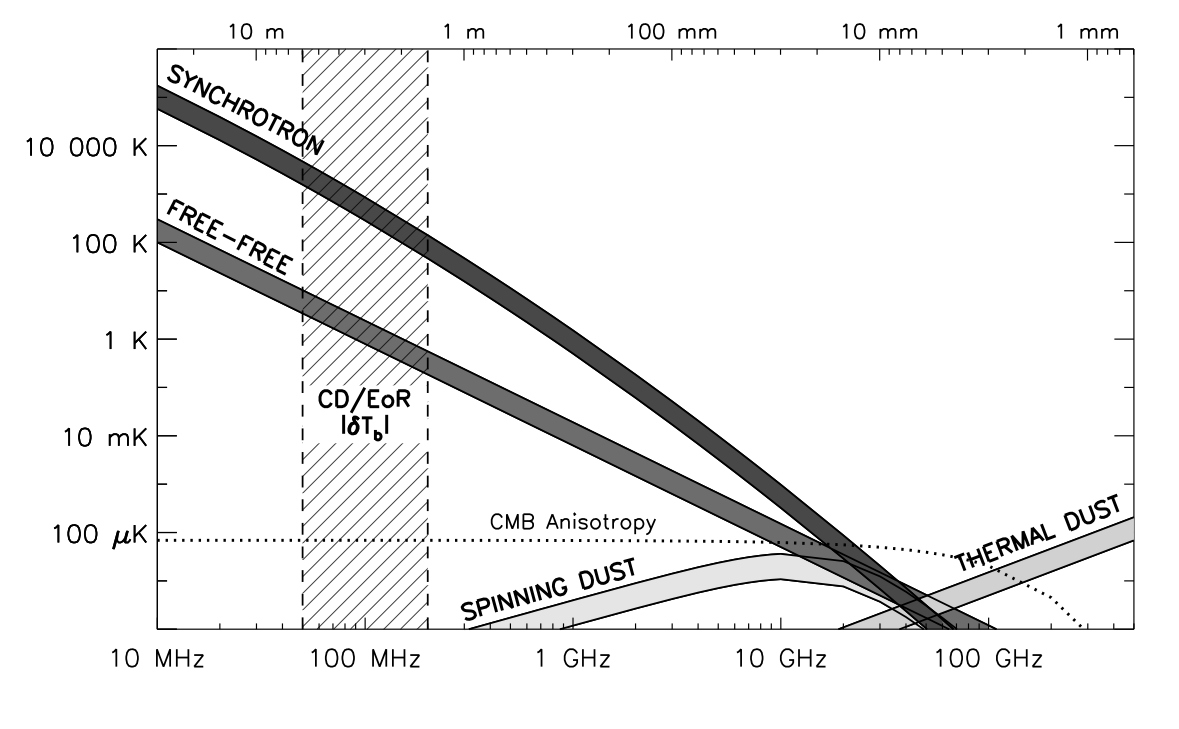
\includegraphics[width=.95\textwidth]{Chapman_Jelic/Images/galcomp.png}
    \caption{The main Galactic diffuse foreground components given as a function of frequency in the total intensity: (i) synchrotron emission from cosmic-ray electrons; (ii) free-free emission from diffuse ionized gas; and (iii) thermal dust emission. There is also a forth component associated with small rapidly spinning dust grains. Synchrotron emission dominates at frequencies below $\sim 10$ GHz, while thermal dust emission dominates at frequencies above $\sim 100$ GHz. Over the whole frequency range of the CD/EoR experiments, Galactic synchrotron emission is 3 -- 4 orders of magnitude stronger in total power (illustrated by the dark grey area) and 2 -- 3 orders of magnitude stronger in fluctuations than the cosmological 21~cm signal ($|\delta T_b|$). In the CMB experiments, on the contrary, there is a sweetspot around $~70$ GHz where the CMB anisotropies are relatively bright compared to the Galactic foreground emission.}
    \label{fig:galcomp}
\end{figure}

For a fairly complete theory of the synchrotron emission  please refer to e.g.~\cite{pacholczyk70,  rybicki86}, while here we outline the basics. The radiated synchrotron power emitted by a single electron is proportional to the square of the electron relativistic kinetic energy, the magnetic energy density, and the pitch angle between the electron velocity and the magnetic field.  The angular distribution of the radiation is given by the Larmor dipole pattern in the electron's frame, but in the observer's frame is beamed sharply in the direction of motion. 

As the electron spirals around the magnetic field, it is in effect accelerating and emitting radiation over a range of frequencies. Its synchrotron spectrum has a logarithmic slope of 1/3 at low-frequencies, a broad peak near the critical frequency $\nu_c$, and sharp fall off at higher frequencies. The critical frequency is directly proportional to the square of the electron energy and the strength of the perpendicular component of the magnetic field. The longer the electron travels, the more energy it losses, the narrower spiral it makes, and the critical frequency is smaller. 

In the case of the Milky Way we need to take into consideration an ensemble of the cosmic-ray electrons, mainly originating from supernovae located close to the Galactic plane and then diffusing outwards. Given a typical magnetic field strength of a few $\mu$G, the cosmic-ray electrons with energies between 0.5 to 20 GeV account for the observed synchrotron radiation from tens of MHz to hundreds of GHz. Their energy spectrum can be approximated with the power law with slope $\delta$:
\begin{equation}\label{eq:ncr}
n_{CR}(E)dE\propto E^{-\delta}dE,
\end{equation}
where $n_{CR}(E)dE$ is the number of cosmic-ray electrons per unit volume with energies between $E$ and $E+dE$. A distribution of their pitch angles is assumed further to be almost random and isotropic due to relatively long timescales (up to several millions of years) over which they lose their relativistic energies and due to repeatedly scattering that occurs in their environments. 

The observed synchrotron spectrum is then given by summing the emission spectra of individual electrons, which are smeared out in the observed spectrum by broad power law energy distribution of the comic-ray electrons. Thus, the synchrotron intensity at frequency $\nu$ depends only on $n_{CR}$ and $\delta$ from Eq.~\ref{eq:ncr} and the strength of the magnetic field component perpendicular to the line-of-sight $B_\perp$:
\begin{equation}\label{eq:Isyn}
I_{\nu}\propto n_{CR}B_\perp^{(\delta+1)/2}\nu^{(1-\delta)/2}.
\end{equation}
The observed $I_{\nu}$ can be also described as a featureless power law in regards to the observed intensity $I_0$ at a reference frequency $\nu_0$:
\begin{equation}
I_{\nu}=I_0\left( \frac{\nu}{\nu_0} \right)^{-\alpha},
\end{equation}
where observed spectral index $\alpha$ is directly connected to the cosmic-ray  index $\delta$ as $\alpha=(\delta-1)/2$. Moreover,  the observed intensity is commonly expressed in terms of the brightness temperature $T_{b}(\nu)\sim\nu^{-\beta}$, using the Rayleigh-Jeans law which holds at radio frequencies. In this case the observed spectral index is $\beta=2+\alpha=2+(\delta-1)/2$. 

The comic-ray energy slope is estimated to  $-3.0<-\delta<-2.5$ at GeV energies \cite{lawson87, strong11, orlando13}. This corresponds to the synchrotron spectral index of $-1<-\alpha<-0.8$ or $-3<-\beta<-2.8$ observed at GHz frequencies \cite{reich88, platania98}.  At MHz frequencies the synchrotron spectrum is flatter \cite{rogers08, guzman11} and references within). Typical values at mid and high Galactic latitudes are $-2.59 < -\beta < -2.54$ between 50 and 100 MHz \cite{mozdzen19} and $-2.62 < -\beta < -2.60$  between 90 and 190 MHz \cite{mozdzen17}, as measured by the EDGES instrument.  

A difference in the spectral index at MHz and GHz frequencies is due to ageing of the cosmic-ray energy spectrum. As the cosmic-ray electrons propagate trough the interstellar medium, they loose their energies by a number of energy loss mechanisms \cite{longair11} that involve interactions with matter, with magnetic fields and with radiation. This then depletes the population of relativistic electrons and changes their original energy (injection) spectra. For example, the energy loss trough synchrotron radiation is larger for cosmic-ray electrons with higher energies ($\sim E_{CR}^2$). The critical frequency is also proportional to $\sim E_{CR}^2$, so over time, the cosmic-ray spectra becomes steeper together with the synchrotron spectra at higher frequencies.  In a similar way, as the cosmic-ray electrons diffuse away from the Galactic plane, the ageing effect also makes a steepening of the synchrotron spectrum at higher Galactic latitudes \cite{strong07}.

Besides the spectral index variations across the sky, brightness temperature variations of the Galactic diffuse synchrotron emission reflect spatial fluctuations of the comic-ray electron density and magnetic field strength in the interstellar medium. Synchrotron emission is hence the brightest along the Galactic plane, where is the largest concentration of supernovae, a major source of the cosmic-ray particles, while the darkest parts are within the halo. This can be seen in \cite{landecker70} all-sky map obtained at 150~MHz (see Fig.~\ref{fig:GDSE}), where typical high latitude brightness is between 150 K and 250 K. Given a low resolution of this map ($\sim5^\circ$), Haslam map at 408~MHz (see Fig.~\ref{fig:GDSE}, \cite{haslam81,haslam82,remazeilles15} is more commonly used as a template for emission at low radio frequencies. 

\begin{figure}[!t]
\centering
    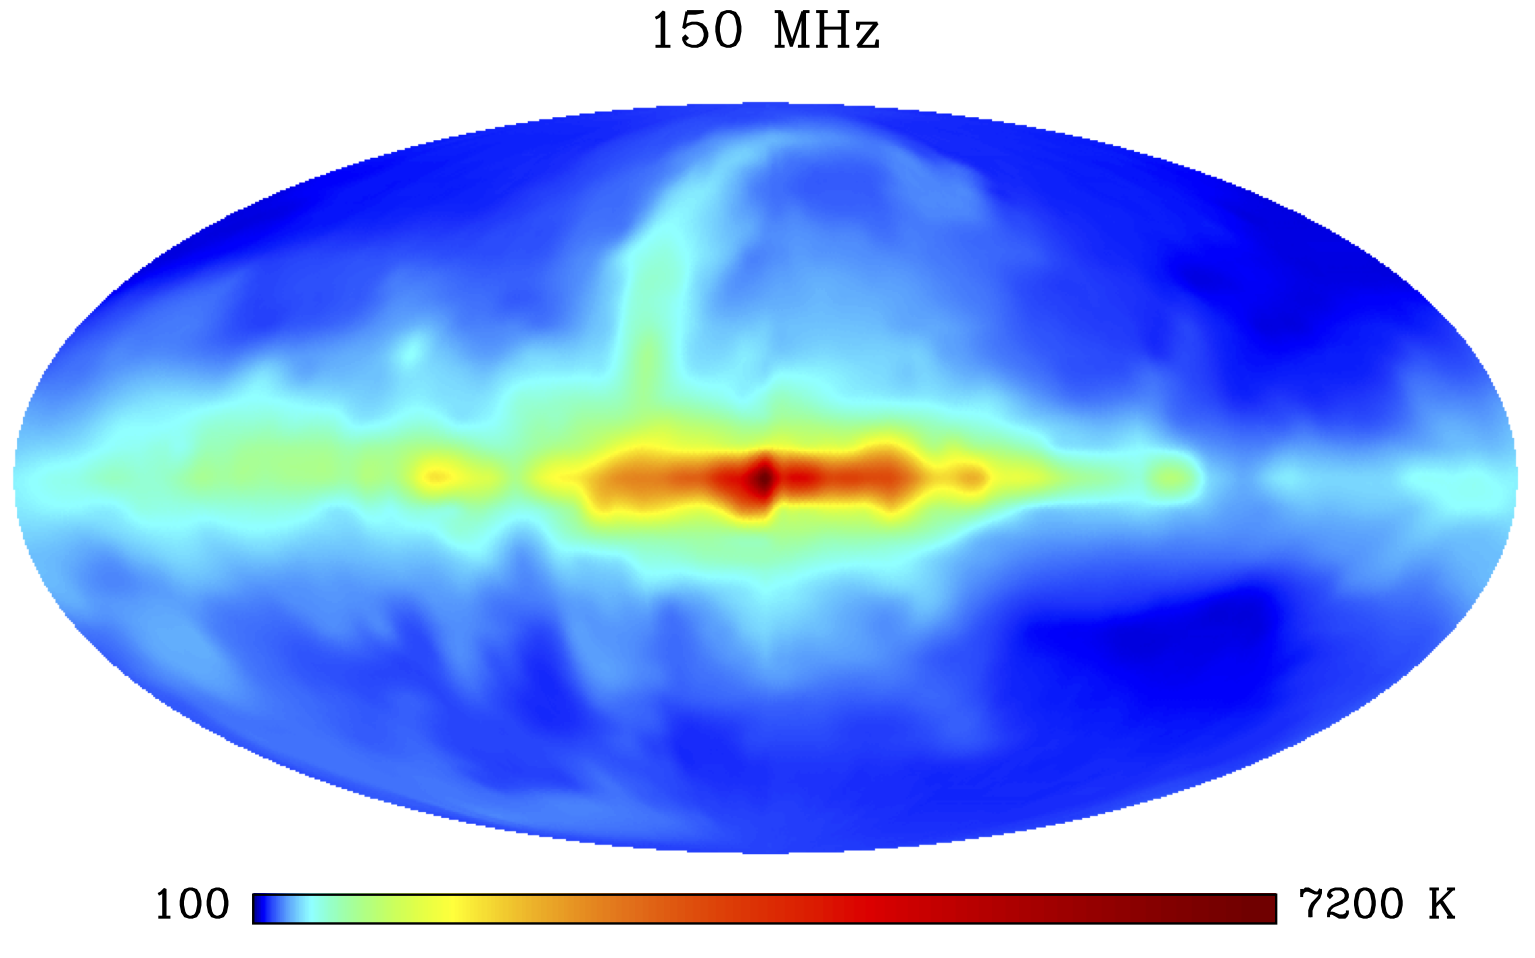
\includegraphics[width=0.475\textwidth]{Chapman_Jelic/Images/landecker.png}
    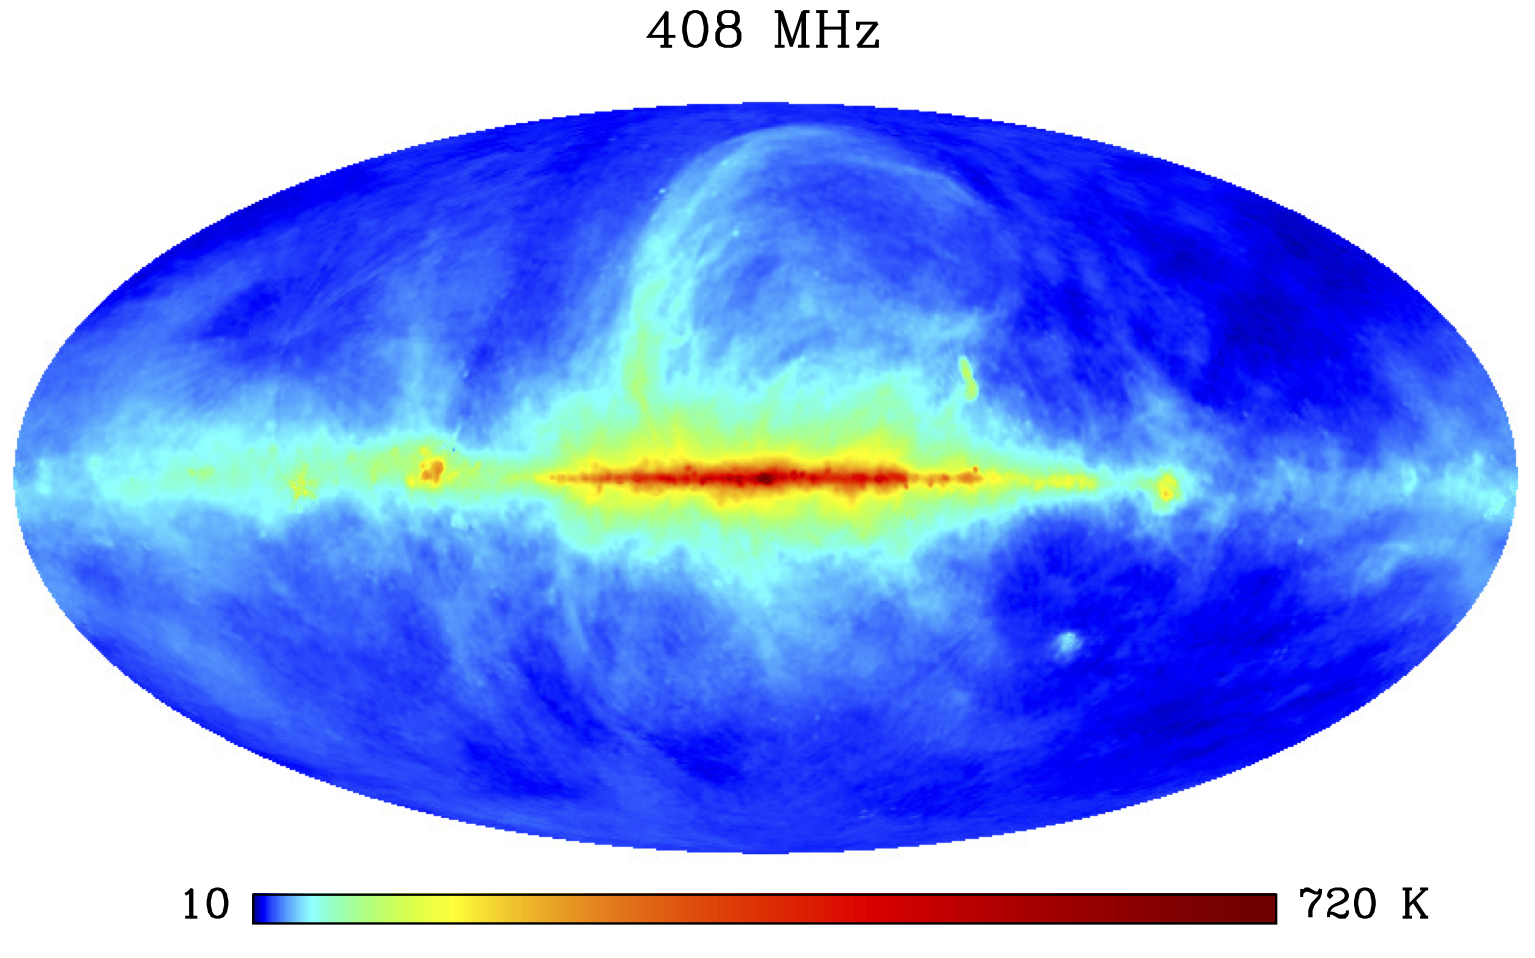
\includegraphics[width=0.475\textwidth]{Chapman_Jelic/Images/haslam.png}
    \caption{All sky maps of Galactic radio emission at 150 MHz \cite{landecker70} and 408 MHz \cite{haslam81, haslam82,remazeilles15}. This data is available on the Legacy Archive for Microwave Background Data Analysis (LAMBDA, https://lambda.gsfc.nasa.gov), a service of the Astrophysics Science Division at the NASA Goddard Space Flight Center.}
    \label{fig:GDSE} 
\end{figure}

A number of recent dedicated observations additionally constrained Galactic synchrotron emission in selected areas at high Galactic latitudes. The WSRT observations at 150 MHz show an excess of power attributed to the diffuse synchrotron with an rms of 3--5~K on scales greater than 30~arcmin (observations of the fields around 3C 196 and the North Celestial Pole \cite{bernardi10}. The LOFAR observation of the North Celestial Pole \cite{patil17} also clearly shows diffuse emission on scales larger than 1 degree, while slightly higher levels are found on scales greater than 54~arcmin in the MWA observations at 154~MHz of the fields near the South Galactic Pole \cite{lenc16}.

\subsection{Extragalactic foregrounds in total intensity}
Extragalactic radio sources have composite nature.  They are mostly the galaxies that have the active galactic nuclei (AGNs) or the star-forming galaxies (SFGs). 

Radio (synchrotron) emission in the AGNs, so called radio--loud AGNs, is related to the accretion of matter by a supermassive black hole at the centre of its host galaxy, typically an elliptical galaxy.  This produces narrow  jets in a direction perpendicular to the plane of the accretion. The jets can be as large as a few to ten times the size 
of the host galaxy and many of them have diffuse endings, so called radio lobes. Observed morphology of radio loud AGNs varies and can be classified in different ways. For example, \cite{fanaroff74} classified them based on their radio luminosity and brightness of their components (nucleus, jets and lobes). FR-I type galaxies have lower radio powers with the edge darkened morphology, while  FR-II type galaxies have higher radio powers with the edge brightened morphology.

Radio emission in the SFGs is produced like in the Milky Way by synchrotron radiation from supernovae related relativistic electrons and by free-free emission from H{\sc ii} regions. Observed radio emission of these galaxies is usually also tightly connected, although still not well understood why, to the observed infrared luminosity measuring the star-formation rate (e.g.\cite{helou85,condon92,jarvis10}), hence the name the SFGs. 

At low--radio frequencies different populations of the radio galaxies are still poorly constrained, especially a faint part of their distribution. There is a low-frequency extragalactic catalogue obtained with the MWA radio telescope in the south (GLEAM, \cite{hurleywalker17}) and the ongoing LOFAR Two-metre Sky Survey (LoTTs,\cite{shimwell17, shimwell19}) in the north. Until we get deeper with these surveys we need to rely on the data obtained at higher radio frequencies.

Normalised differential source counts for different populations of radio sources at 1.4 GHz is given in Fig.~\ref{fig:extragal}. Thanks to the recent very deep surveys (e.g. COSMOS, \cite{bondi08, smolcic17a, smolcic17b, smolcic17c} the extragalactic radio sources are constrained well up to the flux densities of $500~{\rm \mu Jy}$. The population of the SFGs dominate at $\mu{\rm Jy}$ levels, while population of the radio loud AGNs dominates at flux densities $\geq1~{{\rm mJy}}$ (for a review see \cite{prandoniIAUS333} and references therein). There is also a third population of the sources detected below $\sim100~{\rm \mu Jy}$, commonly referred to as radio--quite AGNs. These sources do not have large scale radio jets and lobes like radio--loud AGNs. They are probably the SFGs hosting also an active nucleus that contributes to the radio emission \cite{delvecchio17}. 

\begin{figure}[!t]
   \centering
    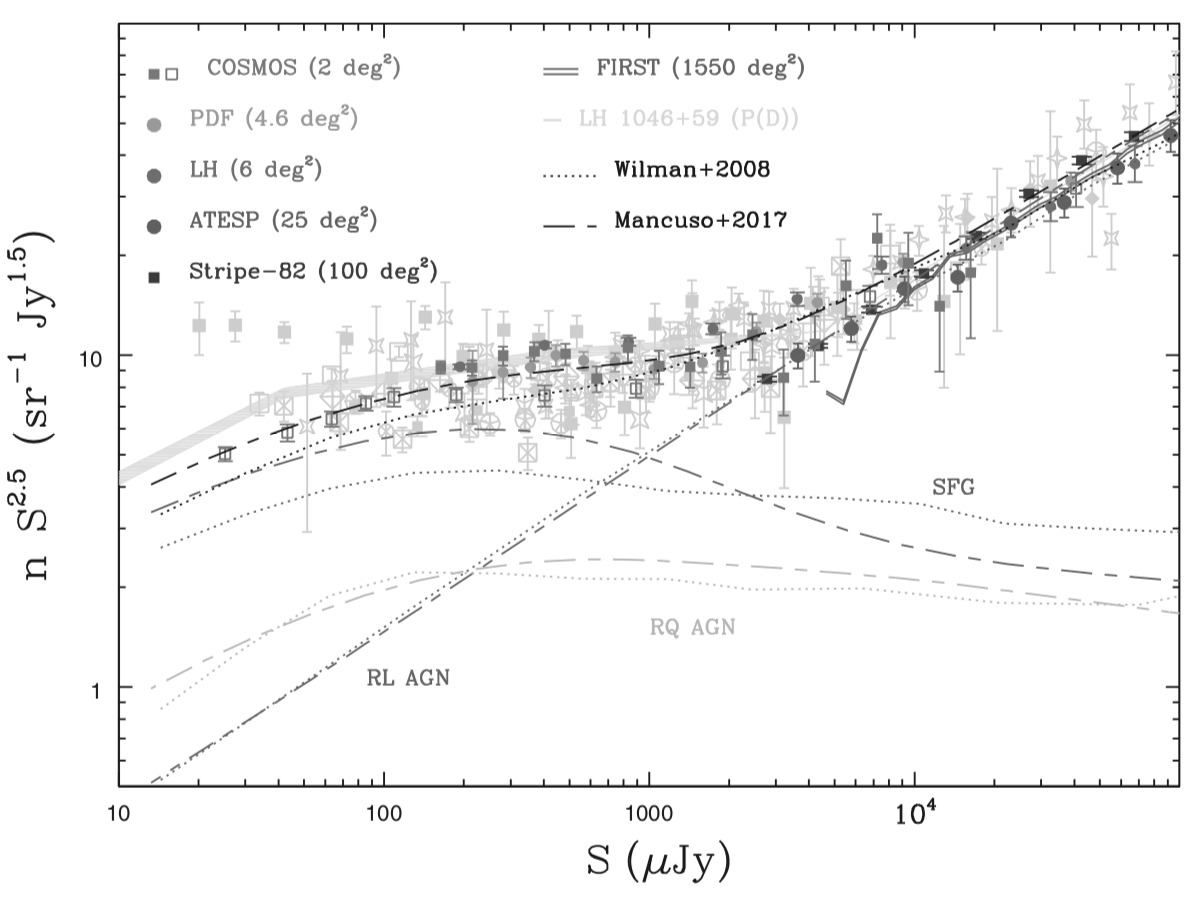
\includegraphics[width=0.95\textwidth]{Chapman_Jelic/Images/extragal.png}
    \caption{Normalized 1.4 GHz differential source counts for different radio source populations (fig. 1 in \cite{prandoniIAUS333}.}
    \label{fig:extragal}
\end{figure}

In addition to the radio source counts we also need to have a good knowledge of their distribution in the sky (clustering properties) and of their radio spectra. Neglecting the source clustering may result in underestimating the angular foreground power which can potentially lead to a false detection of the cosmological 21 cm signal \cite{murray17, murray18}, while if the radio spectra is not smooth the foreground removal will be much more demanding.

The radio spectra of the radio galaxies can be described with the power-law function with a spectral index of  $\alpha\sim-0.7/-0.8$, due to the synchrotron nature of the emission.  Nevertheless, there are process that can change the shape of the spectra (free-free absorption, synchrotron self-absorption, spectral ageing, etc.) and make it complicated. Recent  LOFAR observations of the Bo\"otes field \cite{calistrorivera17} showed significant differences in the spectral curvature between SFG and AGN populations. The radio spectra of SFGs show a weak but statistically significant flattening, while the radio spectra of the AGNs is becoming steeper towards  the lower frequencies. Therefore, different power-law slopes should be assumed for AGNs and SFGs, when modelling the radio sky at frequencies relevant for the cosmological 21 experiments.

\subsection{Polarized foregrounds}\label{sec:polarfg}
Galactic synchrotron emission is partially linearly polarized. Its polarized intensity $PI_\nu$ depends on a cosmic-ray electron density $n_{CR}$, a slope of the cosmic-ray energy spectrum $\delta$, and a strength of the magnetic field component perpendicular to the line-of-sight $B_\perp$, in the same way as defined by Eq.~\ref{eq:Isyn} in total intensity. The only difference is the amount of emission, defined by the degree of polarization \cite{rybicki86}:
\begin{equation}
\Pi=\frac{\delta+1}{\delta+7/3}.
\end{equation}
For $p=2.2$, which is consistent with the observed synchrotron spectral index of $-\beta=-2.6$ at 150 MHz \cite{mozdzen17}, we get $\Pi=0.7$. At low radio frequencies  (100--200~MHz) about $70\%$ of Galactic synchrotron emission is intrinsically polarised, while in fact we observe only a few percent \cite{bernardi13, jelic14, jelic15, lenc16, vaneck17,vaneck19}. To understand why we observe such a small percentage of polarised emission, we need to take a closer look at Faraday rotation and associated depolarisation that occurs. 

As linearly-polarised wave, with a wavelength $\lambda$, propagates through a magnetised plasma its polarisation angle $\theta$ is Faraday rotated by:
\begin{equation}\label{eq:FR}
\frac{\Delta \theta}{\rm [rad]}= \frac{\lambda^2}{\rm [m^2]}\frac{\Phi}{\rm [rad~m^{-2}]}=  \frac{\lambda^2}{\rm [m^2]}\left(0.81\int \frac{n_e}{\rm [cm^{-3}]} \frac{B_{||}}{\rm [\mu G]} \frac{dl}{\rm [pc]}\right),
\end{equation}
where $\Phi$ is Faraday depth, $n_e$ is a density of the thermal electrons, $B_{||}$ is a strength of the magnetic field component parallel to the line-of-sight. The integral is taken over the entire path-length $l$, from the source to the observer.  The Faraday depth is positive when $B_{||}$ points towards the observer, while it is negative when $B_{||}$ points away.

In the Milky Way, where distributions of thermal and comic-ray electrons are perplexed throughout the entire volume, differential Faraday rotation will occur and will depolarise the observed synchrotron emission \cite{sokoloff98}.  As Faraday rotation is proportional to $\lambda^2$, depolarisation at low radio frequencies will be significant. 
Nevertheless, small amounts of polarised emission that can still be observed carries valuable information about the physical properties of the intervening magnetised plasma.

\begin{figure}[!h]
\centering
    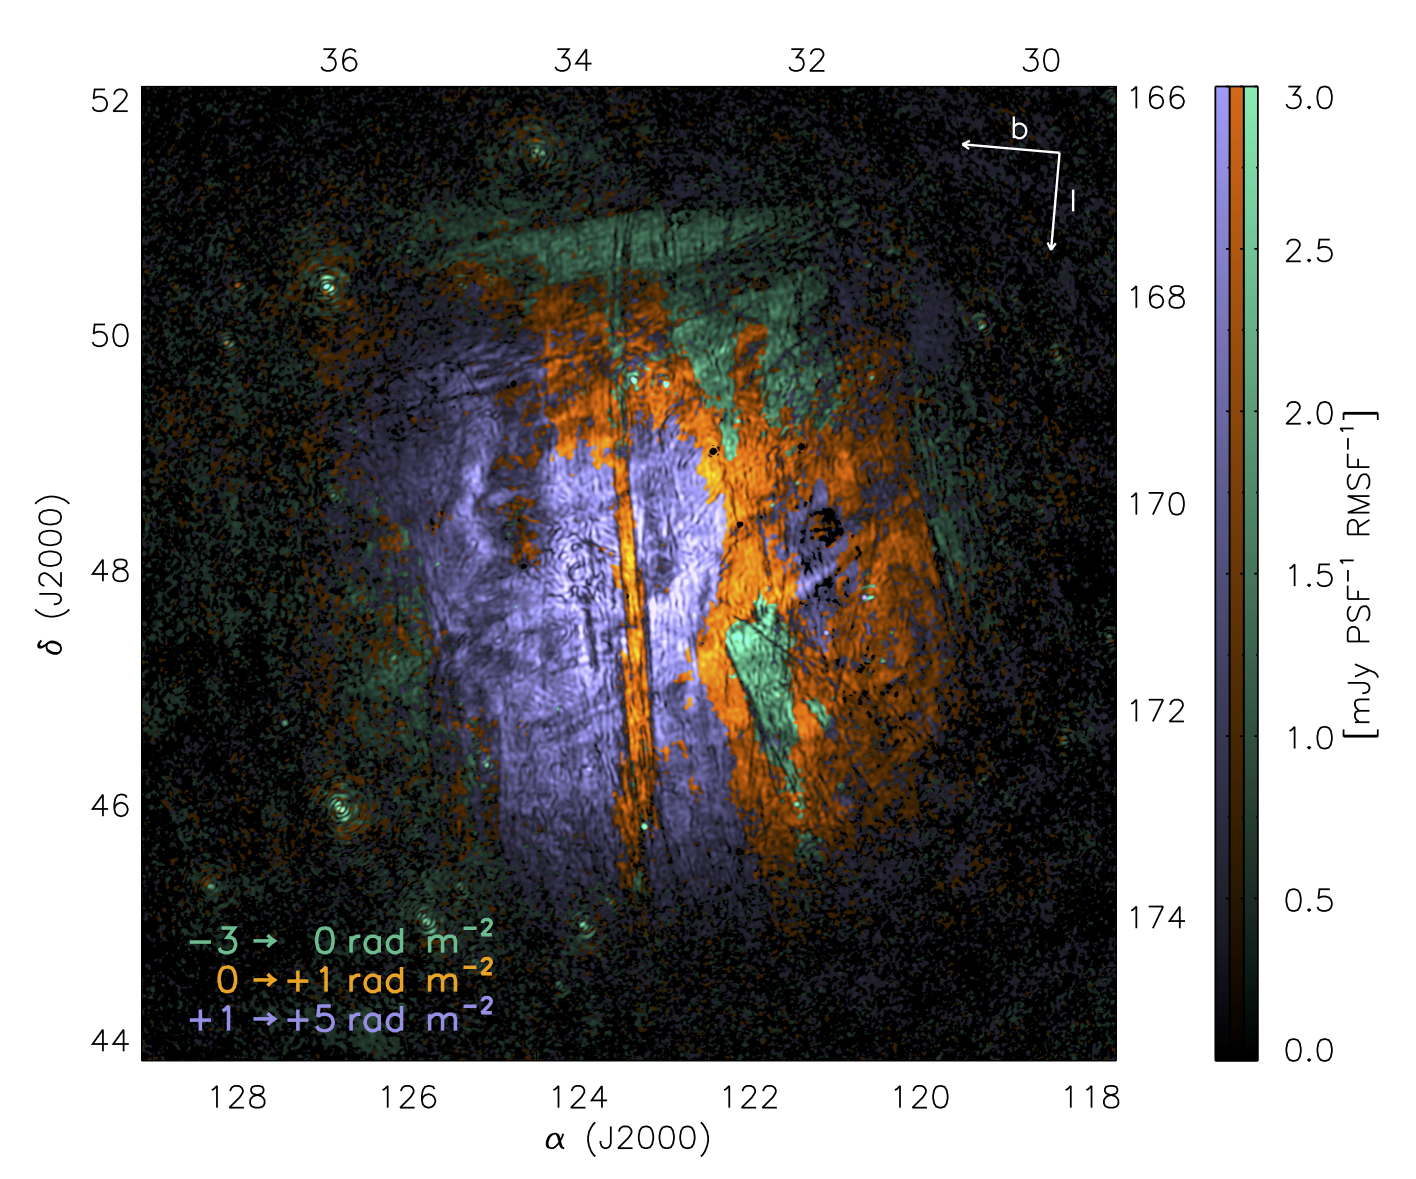
\includegraphics[width=0.475\textwidth]{Chapman_Jelic/Images/3C196.png}
    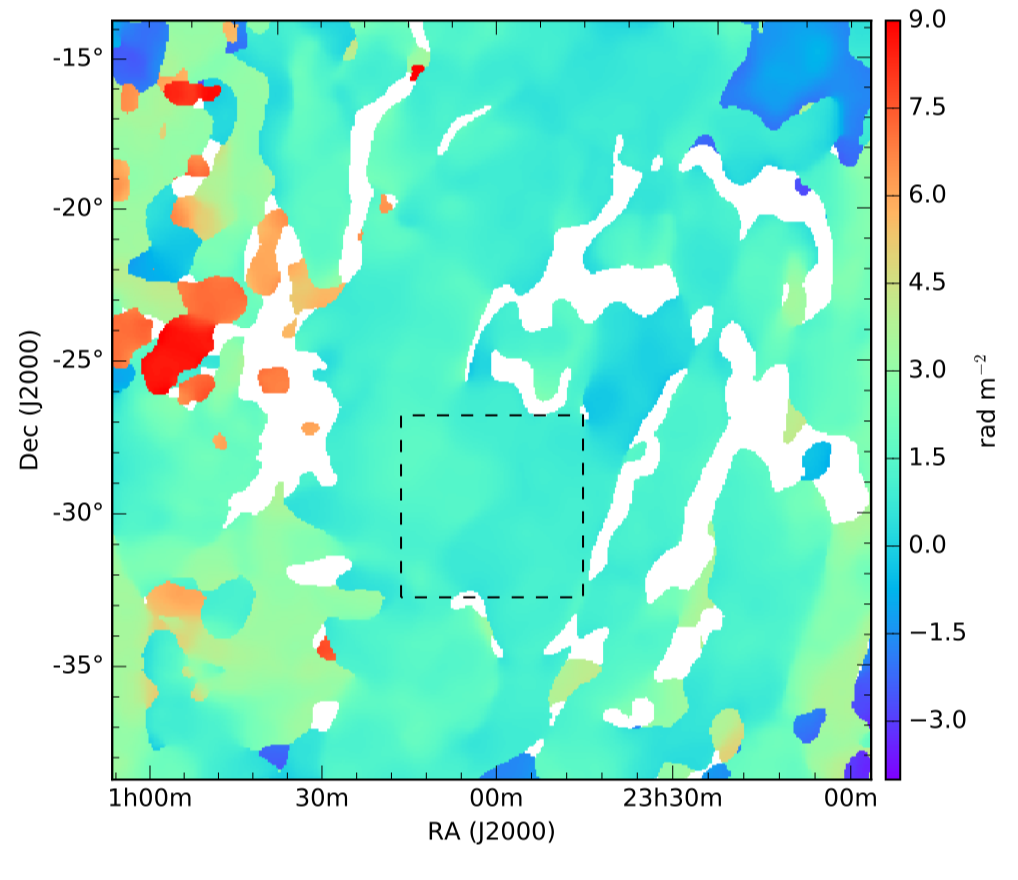
\includegraphics[width=0.475\textwidth]{Chapman_Jelic/Images/lenc.png}
    \caption{Polarised structures discovered with LOFAR (\% cite{jelic15} and MWA \cite{lenc16}
      in two fields at high Galactic latitudes.}
    \label{fig:polar}
\end{figure}


First attempts to constrain diffuse polarised emission at 150 MHz were done using the GMRT \cite{pen09} and WSRT observations \cite{bernardi09, bernardi10}.  However, the full richness and complexity of polarised emission at low-radio frequencies was not revealed until LOFAR and MWA came online.  Observations with these instruments discovered astonishing morphology of polarised Galactic synchrotron emission of a few Kelvin in brightness (and see Fig.~\ref{fig:polar} \cite{bernardi13, iacobelli13b, jelic14, jelic15, lenc16, vaneck17,vaneck19}. Discovered structures were unraveled by Rotation Measure (RM) synthesis \cite{brentjens05}. This is a technique in radio polarimetry that disentangles the observed wavelength-dependent polarisation into Faraday spectrum, i.e., the distribution of polarised emission as a function of Faraday depth. This allow us then to preform, so called, Faraday tomography, a study of the intervening magnetised plasma as a function of Faraday depth.

Given a wide frequency coverage and a high spectral resolution available in the low-frequency instruments Faraday tomography is preformed at an exquisite sensitivity and resolution in Faraday depth of $\sim1~{\rm rad~m^{-2}}$, an order of magnitude higher than at 350 MHz. This allow us to map small column densities of magnetised plasma that are, in most cases, not possible to detect at higher radio frequencies. Interestingly, most of the observed structures at low-radio frequencies appear at Faraday depths $\Phi\leq15~{\rm rad~m^{-2}}$ and they are not correlated with structures in total intensity. This result will be relevant in later discussion of polarisation leakage in the cosmological 21~cm experiments (see Sec.~\ref{sec:leakage}).

Extragalactic polarised sources are not a big concern for the cosmological 21~cm experiments due to their sparsity in the sky. \cite{bernardi13} surveyed 2400 deg$^2$ of the southern sky at 189 MHz with the MWA 32-element prototype and found only one polarised source. In a preliminary data realise of the LOFAR Two-meter Sky Survey of the HETDEX field, covering an area of 570 square degrees, 92 polarized radio sources where found \cite{vaneck18}. This gives a lower limit to the polarized source surface density at 150 MHz of only 1 source per 6.2 square degrees. Something higher value, 1 source per 2 degrees, is found based on three LOFAR observations of three 16 deg$^2$ fields \cite{mulcahy14, jelic15, vaneck18}.
 
\section{Foreground Mitigation}
%%% COMMENTED OUT TEXT IS PROBABLY IRRELEVANT DUE TO PREVIOUS CHAPTERS %%%
%Current and future efforts to provide direct observational insight into the Epoch of Reionization have largely focused on detecting the 21-cm radiation emitted by the neutral hydrogen pervading the Universe at high redshifts. At lower redshifts when the first ionizing sources have begun to ionize bubbles in the neutral hydrogen, the 21-cm signal is diminished until, as those bubbles overlap and entirely ionize the Universe, the 21-cm signal depletes entirely. 

The 21-cm signal emitted by high-redshift neutral hydrogen provides a window into the Epoch of Reionization (EoR), but it is a window that is obscured by layers of foregrounds. Terrestrially, radio frequency interference (RFI) from any human-made sources of radio transmission, such as wind turbines, leads to the necessary excision of frequency channels using a flagging technique (e.g. \cite{Prasad2012ExA....33..157P,Offringa2012}. The number of channels excised is significant, around 1$\%$ of channels of data for MWA and LOFAR \cite{Offringa2019MNRAS.484.2866O,Offringa2015PASA...32....8O}. Without careful mitigation in the calibration, imaging and diffuse foreground removal stages, RFI excision can result in an excess power that scales with the number of excised channels and does not integrate down with time, significantly dominating over the cosmological 21-cm signal by 1-2 magnitudes \cite{Offringa2019MNRAS.484.2866O}. Extra-terrestrially, there exist a multitude of foregrounds which dominate all frequencies of observation and so more subtle methods than excision are required. This part of the chapter discusses the development and current use of Galactic and extragalactic foreground mitigation methods in Epoch of Reionization 21-cm experiments.


\subsection{Foreground Mitigation in the Data Analysis Pipeline}
\subsubsection{Bright Source Removal}
The first stage of foreground removal involves mitigating the effect of the very brightest sources on the sky: the point sources and extended sources. Bright source removal often comes under the umbrella of calibration as opposed to foreground mitigation however we will briefly summarize the process here. For example, the MWA real-time system (RTS) \cite{Mitchell2008ISTSP...2..707M} carries out sequential bright source `peeling' on the visibilities, tracking a few hundred of the brightest sources and comparing to a sky model constructed from existing catalogues and MWA observations \cite{Carroll2016MNRAS.461.4151C}. The gains are calibrated on the strongest source, before that source is peeled (subtracted) from the data, and the next strongest source is used to refine the calibration, and so on until it is deemed that enough bright sources have been removed, usually a few hundred to a thousand at most. The other MWA calibration pipeline, Fast Holographic Deconvolution (FHD) \cite{Sullivan2012ApJ...759...17S}, uses the MWA extragalactic catalogue GLEAM \cite{hurleywalker17} to calibrate gains, modelling all sources out to 1$\%$ beam level in the primary lobe, amounting to approximately 50000 sources \cite{Barry2019arXiv190102980B} and then removing a smaller population of them from the data. Similarly, LOFAR has built up a sky model over several years using the highest resolution LOFAR images and subtracts the sources in visibility space also \cite{Yata2015MNRAS.449.4506Y,Yata2013AA...550A.136Y}. As of 2017, the LOFAR EoR sky model contained around 20,800 unpolarized sources. 

\subsubsection{The EoR Window}
\label{sec:wedge}

It has previously been traditional when discussing diffuse foreground mitigation to assume that the previous stage of bright source subtraction has already been implemented perfectly. This is no longer seen to be a valid or safe assumption, as the chromaticity of the instrument, calibration errors and incorrect source subtraction lead to significant bias in the EoR signal for all current and planned experiments (e.g. \cite{ EW2017MNRAS.470.1849E,Procopio2017PASA...34...33P,Barry2016MNRAS.461.3135B,Patil2016MNRAS.463.4317P,Datta2010ApJ...724..526D,Liu2009MNRAS.394.1575L}, including redundant arrays \cite{Byrne2019ApJ...875...70B}. 

\begin{figure}
\begin{center}
    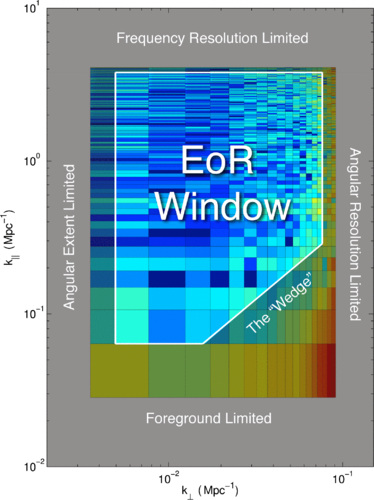
\includegraphics[width=0.5\textwidth]{Chapman_Jelic/Images/medium.png}
\end{center}
    \caption{A schematic of the `EoR Window' in the cylindrical $k_{\parallel}$,$k_{\perp}$ Fourier plane, taken from Fig.1 of \cite{Dillon2014PhRvD..89b3002D}. In a perfect observation, with zero instrumental effects, the foregrounds would be entirely contained in the well defined horizontal band. In a realistic observation however, the chromaticity of the instrument results in a leakage of power up into the EoR window, into a region called the `wedge'. Aside from these contaminated areas there should be a relatively clean area called the EoR window.}
    \label{fig:window_liu}
\end{figure}

The spectral differences between the EoR signal and the bias introduced by the foregrounds and instrument lend themselves to a neat separation in $k_\bot-k_\parallel$ space, Fig. \ref{fig:window_liu}. In this formalism, spectrally-smooth foregrounds live in a well-defined area of $k$-space, at the smallest $k_\parallel$ scales, equivalent to the red stripe at the bottom of Fig. \ref{fig:window_liu}, excluding the wedge area. The assumption that the foregrounds would remain smooth and confined in a horizontal area at low $k_\parallel$ even after observation by a radio interferometer drove early foreground removal techniques such as those introduced in Section \ref{sec:poly} but is now known to be an incorrect assumption. The chromaticity of the instrument results in a `mode-mixing' where power is transferred from the angular to the frequency scales, throwing power upwards from the foreground area in the window into the larger $k_\parallel$ scales, with the effect increasing with larger $k_\bot$. This results in a wedge like structure, a structure that has been now extensively discussed and mathematically defined in the literature (e.g. \cite{Jensen2016MNRAS.456...66J,Dillon2014PhRvD..89b3002D,Liu2014PhRvD..90b3019L,Liu2014PhRvD..90b3018L,Hazelton2013ApJ...770..156H,Thyagarajan2013ApJ...776....6T,Pober2013ApJ...768L..36P,Morales2012ApJ...752..137M,Vedantham2012ApJ...745..176V,Trott2012ApJ...757..101T,Parsons2012ApJ...756..165P,Datta2010ApJ...724..526D}. Because the point sources reside on the largest $k_\bot$ scales they, or even their residuals when incorrectly calibrated, can overwhelm the EoR power in the frequency scales (e.g. \cite{Bowman2009ApJ...695..183B} and immediately preceding references).

Now we have defined the problem, namely the overpowering magnitude and potential leakage of foregrounds onto the EoR signal, we can consider how to achieve our aim of making accurate statistical conclusions on the nature of the EoR using the data within this window. To proceed, we can consider two philosophies. The first, \textbf{foreground subtraction}, aims to remove foreground contamination on all scales. The benefit of this is that there are more $k$ scales available for analysis. The drawback of foreground subtraction across all $k$-scales is that any failure in the method will potentially result in a foreground fitting bias across all scales of the window, providing another layer of contamination. One could instead avoid the foregrounds and therefore the need to remove them: \textbf{foreground avoidance}. This philosophy aims to then quantify the foregrounds and wedge such that any analysis occurs within a well-defined window free of contamination. The benefit of this is, as stated, the avoidance of foreground subtraction bias. The drawback is that any analysis is performed on a significantly reduced set of scales which can for example introduce its own bias into the spherically averaged power spectrum \cite{Jensen2016MNRAS.456...66J}. Additional to both philosophies, we can implement \textbf{foreground suppression}, which down-weights scales where the foregrounds or foreground removal residuals are dominant. We will now discuss these approaches in further detail in the context of current EoR experiments.

\subsection{Foreground Avoidance and Suppression}

The Murchison Widefield Array (MWA) has two separate pipelines which differ in their application of foreground mitigation techniques and calibration methods, while mostly employing foreground avoidance. They way in which MWA is optimized for making images allows the option to directly subtract known foregrounds but in this case the direct foreground subtraction is primarily applied to get access to a cleaner EoR window, not to get access to within the wedge, as is the motivation of foreground subtraction in LOFAR.

\begin{figure}
\begin{center}
    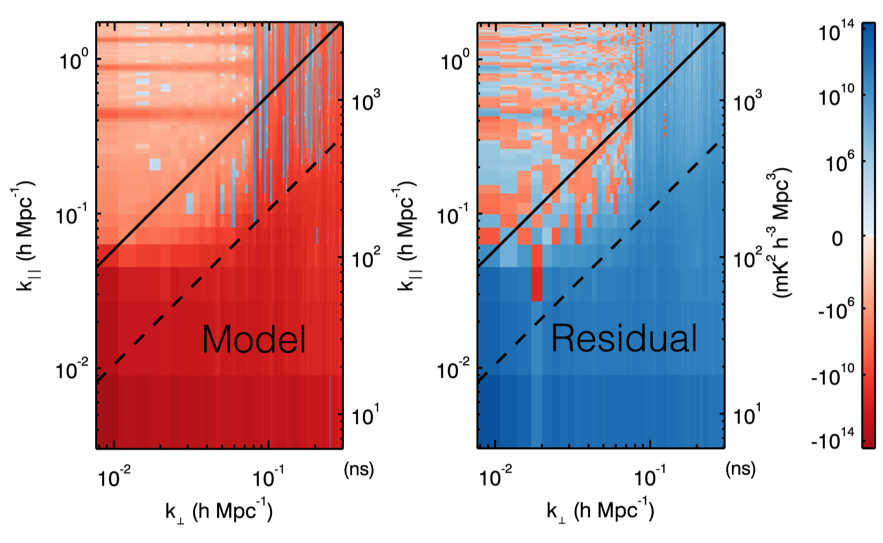
\includegraphics[width=0.9\textwidth]{Chapman_Jelic/Images/apjaa3b64f9_hr.png}
\end{center}
\caption{Left: MWA foreground model without diffuse foregrounds (i.e. just point sources) and with diffuse foregrounds. Adding diffuse foregrounds into the model produces leakage far up into the EoR window and instrumental contamination can be seen in the horizontal lines throughout the EoR window. Right: the difference between the power spectrum of the residuals when only the point sources have been subtracted as described above, and the power spectrum of the residuals where the diffuse foregrounds have also been subtracted. There is a clear reduction in foreground residuals all along the wedge and the EoR window is noise-like, suggesting a lack of foreground contamination there. There is a 70$\%$ reduction in residual power of the foregrounds using this method. Figure taken from \cite{Beardsley2016ApJ...833..102B}.}
    \label{fig:beardsley_fg_sub}
\end{figure}

The FHD \cite{Sullivan2012ApJ...759...17S} and $\epsilon$psilon \cite{Barry2019arXiv190102980B} pipeline builds a sky model of point sources based on a golden set of data, including all sources above a floor limit within the primary beam of the instrument, and those beyond the primary beam if they are above 1$\%$ of the maximum primary beam level. This point source model is used in calibration in a similar way to LOFAR, and contains about 7000 sources as of 2016 \cite{Beardsley2016ApJ...833..102B}. In contrast to the RTS \cite{Mitchell2008ISTSP...2..707M} and CHIPS \cite{Trott2016ApJ...818..139T} pipeline, the FHD-$\epsilon$psilon pipeline also generates a diffuse foreground model by subtracting away the point source model from the observed data, and integrating over frequency to create a diffuse foreground model free of spectral information \cite{Beardsley2016ApJ...833..102B}. They then subtract both the point source model and the diffuse model from the data to minimise the leakage from the wedge into the EoR window. In Fig \ref{fig:beardsley_fg_sub} we see the effect of this foreground subtraction on the EoR window. The left image is the difference between the power spectrum of the MWA foreground model without diffuse foregrounds (i.e. just point sources) and with diffuse foregrounds. The plot shows that the diffuse foregrounds have power far up into the EoR window, due to non-uniform spectral sampling and the effect of windowing the data along frequency during the Fourier Transform. This figure if no other demonstrates the danger of assuming that the observed foreground signal is smooth and contained only at the smallest $k_\parallel$. Further instrumental complications can be seen in the horizontal lines throughout the EoR window, which is contamination due to the periodic frequency sampling function used by MWA \cite{Offringa2016MNRAS.458.1057O}. The right plot of Fig. \ref{fig:beardsley_fg_sub} shows the difference between the power spectrum of the residuals when only the point sources have been subtracted as described above, and the power spectrum of the residuals where the diffuse foregrounds have also been subtracted. There is a clear reduction in foreground residuals all along the wedge and the noise-like characteristic of the EoR window suggests a lack of foreground contamination there. \cite{Beardsley2016ApJ...833..102B} report a 70$\%$ reduction in residual power of the foregrounds using this method.

The black lines in Fig. \ref{fig:masks} show the area of the EoR window used in the FHD-$\epsilon$psilon pipeline, with the masks ensuring the avoidance of the horizontal contamination lines and the wedge.

\begin{figure}
\begin{center}
    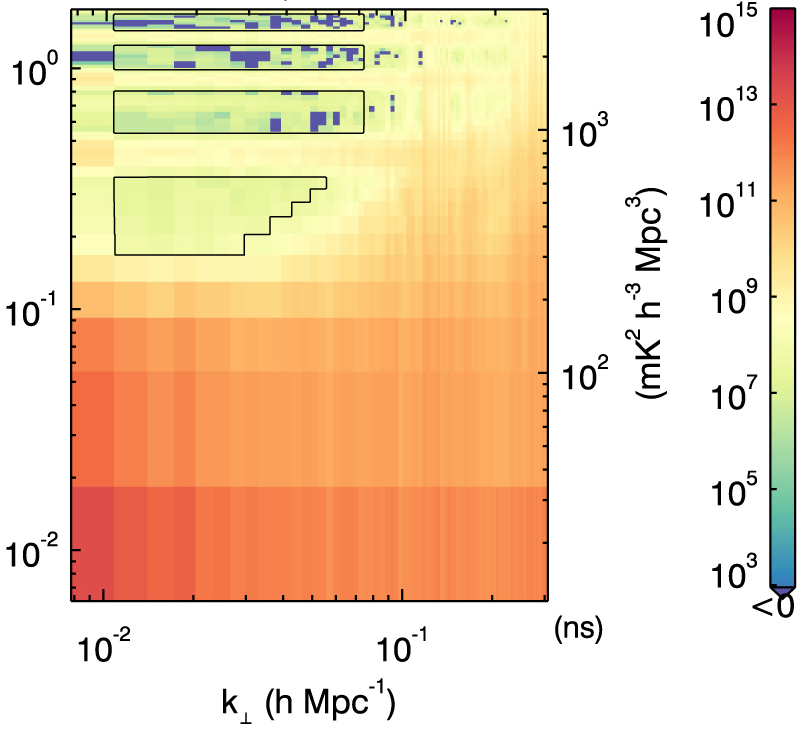
\includegraphics[width=0.9\textwidth]{Chapman_Jelic/Images/apjaa3b64f13_hr.jpg}
\end{center}
    \caption{An example 2D cylindrical power spectrum of the first season MWA data after foreground mitigation. The data used for the upper limits can be seen bounded by black lines. The amount of data available for a power spectrum analysis has been severely reduced by the presence of foregrounds and instrumental contamination but the data within the bounded regions displays noise-like behaviour indicative of successful foreground mitigation. Figure taken from \cite{Beardsley2016ApJ...833..102B}.}
    \label{fig:masks}
\end{figure}

The RTS-CHIPS pipeline subtracts significantly fewer sources, a few hundred to a thousand at most, and does so in visibility space. There is no diffuse foreground model in the subtraction stage and instead CHIPS down-weight modes with residual point source power. There is also the option of diffuse foreground weighting based on a simple foreground model where the covariances are known, though in practice this diffuse down-weighting is not currently utilised.

\subsubsection{Delay Space Filtering}
Delay space filtering is a method of foreground avoidance primarily adopted by the Donald C. Backer Precision Array for Probing the Epoch of Reionization (PAPER) \cite{Parsons2010AJ....139.1468P}. As with most foreground mitigation methods it requires the foregrounds to be reasonably smooth, even after instrumental effects. The wedge is the end-result of an instrument where the frequency-dependence of the instrument's sampling is dependent on the length of the baseline measuring the sky. Delay-space filtering exploits this relation by analyzing the data per baseline, circumventing the conspiracy of instrumental effects on the foregrounds and effectively isolating the foregrounds such that they are easily avoided. Fig. \ref{fig:baselines} demonstrates that for a given baseline measurement the visibility sampled changes with frequency, with a steeper change for longer baselines. This results in the mode-mixing seen in the 2D cylindrical power spectrum and the wedge structure, where we see power thrown up into the EoR window increasingly on the largest $k_\bot$ scales, which are the scales sampled by the longest baselines. Delay space filtering aims to mitigate the mode mixing by performing a Fourier transform along the visibility sampled by a given baseline (a solid line in Fig. \ref{fig:baselines}, and not along the frequency direction (vertical axis of Fig. \ref{fig:baselines}as is usual.

\begin{figure}
\begin{center}
    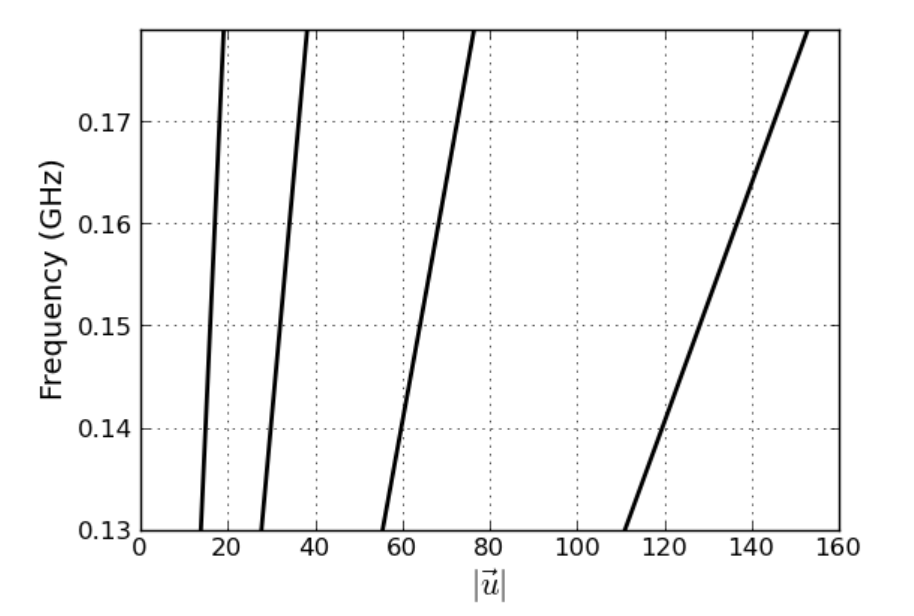
\includegraphics[width=0.5\textwidth]{Chapman_Jelic/Images/baselines.png}
\end{center}
    \caption{This figure, taken from \cite{Parsons2012ApJ...756..165P}, demonstrates the frequency dependence of the wavemode sampled by baselines measuring 16, 32, 64, and 128 wavelengths at 150 MHz. For a given baseline measurement, the visibility sampled changes with frequency, with a steeper change for longer baselines. This results in the mode-mixing seen in the 2D cylindrical power spectrum and particularly "the wedge", where we see power thrown up into the EoR window increasingly on the smallest $k_\bot$ scales, which are the scales sampled by the longest baselines.}
    \label{fig:baselines}
\end{figure}

A delay transform takes a single time sample of a visibility from one baseline, for all observed frequencies (i.e. one of the solid lines on Fig. \ref{fig:baselines}, and Fourier transforms it to produce the delay spectrum \cite{Parsons2012ApJ...756..165P,Parsons2012ApJ...753...81P,Parsons2009AJ....138..219P}. The delay transform is:

\begin{equation}
    \widetilde{V}_b(\tau) = \int dl \; dm \; d\nu \; A(l,m,\nu)I(l,m,\nu)e^{-2\pi i\nu(\tau_g-\tau))}
\end{equation}

\noindent where $l,m$ have their usual definition relating to angular coordinates on the sky (e.g. \cite{Thompson2001isra.book.....T}). $\tau$ is the time-delay between the signal reaching both antennas and the geometric group delay associated with the projection of baseline $\overrightarrow{b} \equiv (b_x,b_y,b_z) $ in the direction $ \hat{s} \equiv (l,m,\sqrt{1-l^2-m^2})$ is:

\begin{equation}
    \tau_g \equiv \frac{\overrightarrow{b} \cdot \hat{s}}{c} 
\end{equation}

For comparison, the usual equation where the Fourier transform is simply applied along the frequency axis is:

\begin{equation}
    \widetilde{V}(u,v,\eta) = \int dl \; dm \; d\nu \; A(l,m,\nu)I(l,m,\nu)e^{-2\pi i(ul+vm+\eta\nu)}
\end{equation}

\noindent where $\eta$ is the Fourier transform of $\nu$.

The delay transform transforms flat spectra sky emission into delta functions. Because the sky emission is not perfectly smooth, and the instrument adds in its own unsmoothing effects, this delta function is effectively convolved with a kernel, which broadens the delta function in delay space. For the smoother foregrounds, that kernel will be narrow, and confined within the ``horizon limits", the geometric limit in delay space beyond which no flat spectra emission can enter the telescope. Spectrally unsmooth sky emission can enter beyond these horizon limits and emission such as the cosmological signal finds itself with a wide convolving kernel, spreading power well beyond the horizon limit where the foregrounds are theoretically confined. In Fig. \ref{fig:horizon} we see the delay transform at 150 MHz for several spectrally smooth sources and how they remain confined within the horizon limits of the baseline (here 32 metres). In contrast, the delay spectrum of spectrally unsmooth emission, such as the cosmological 21-cm signal, finds itself smeared to high delays. Full mathematical detail can be found in \cite{Parsons2012ApJ...756..165P,Parsons2012ApJ...753...81P} and \cite{Parsons2009AJ....138..219P}.

\begin{figure}
\begin{center}
    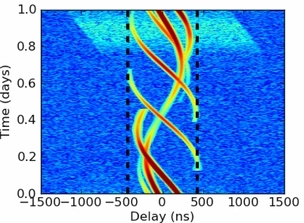
\includegraphics[width=0.5\textwidth]{Chapman_Jelic/Images/horizon.jpg}
\end{center}
    \caption{The delay spectra of several smooth-spectra sources, which remain largely confined within the geometric horizon limits. The broad 21-cm cosmological signal delay spectra in cyan demonstrates that unsmooth spectral signals have a much wider convolving kernal and produce a much wider delay spectra. If analysis is carried out outside of the horizon limits then the foregrounds can be avoided. Taken from \cite{Parsons2012ApJ...756..165P}.}
    \label{fig:horizon}
\end{figure}

By performing this delay space transform, we are effectively moving into the sidelobes of the 21-cm signal in delay space. The cosmological signal is scattered to high delays whereas the foregrounds are not, allowing the data analysis in that large delay space to be free of foregrounds and foreground removal bias. This method also removes the need for imaging in order to remove the foreground directly, making it suitable for a redundant array with little or no ability to image, but a high sensitivity to the 21-cm power spectrum \cite{Parsons2012ApJ...753...81P}.   

PAPER is a radio interferometer with a highly redundant antenna layout, with multiple baselines of the same length and orientation. Because these multiple baselines all measure the same sky signal, any differences in the signal received would be due to instrumentation, allowing a quick calibration for multiple calibration parameters - `redundant calibration' (e.g. \cite{Ronniy2018AJ....156..285J,Li2018ApJ...863..170L,Dillon2016ApJ...826..181D,Zheng2014MNRAS.445.1084Z,Wieringa1992ExA.....2..203W}). 

PAPER avoided the use of the delay modes dominated by foregrounds and downweighted residual foregrounds using inverse covariance weighting in order to form an upper limit power spectrum measurement \cite{Ali2015ApJ...809...61A}. The latter method of inverse covariance weighting where the covariance is calculated based on the data itself has now been shown to carry the considerable risk of overfitting the EoR data \cite{Cheng2018ApJ...868...26C}. To be clear, despite the retraction of the PAPER-64 results due to power spectrum estimation errors \cite{Ali2018ApJ...863..201A}, the delay space filtering technique remains a promising approach to foreground mitigation.

\subsection{Foreground Subtraction}
Foreground subtraction methods all seek to find a model for the observed foregrounds and remove that model from the observed signal, leaving the cosmological signal, instrumental noise and any foreground fitting errors. Foreground removal is usually applied on all scales, meaning that it potentially allows access into the lowest $k_\parallel$ scales where foregrounds traditionally dominate. A caveat of this is that any foreground fitting bias has the potential to affect all scales in the window: foregrounds may remain within the wedge and cosmological signal may be erroneously fitted out within the previously clean EoR window. As an aside, there has been no method so far that can separate out the cosmological 21-cm signal entirely by itself, separate from instrumental noise. Currently when the foregrounds are subtracted or avoided the cosmological noise and signal are still mixed together in what are often termed the `residuals'. The instrumental noise can be obtained from the data for example by the differencing of very fine bandwidth frequency channels, such that both the foregrounds and EoR signal are smooth. The noise power spectrum can then be removed from the residual power spectrum to form the recovered cosmological signal power spectrum. We will now introduce some of the main foreground subtraction techniques.

\subsubsection{Polynomial Fitting and Global Experiments}
\label{sec:poly}

\begin{figure}
\begin{center}
    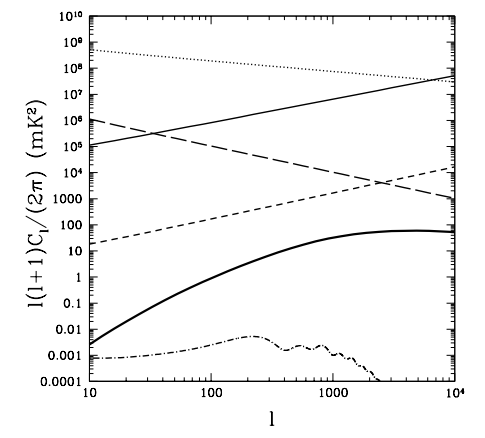
\includegraphics[width=0.4\textwidth]{Chapman_Jelic/Images/santos_spat.png}
    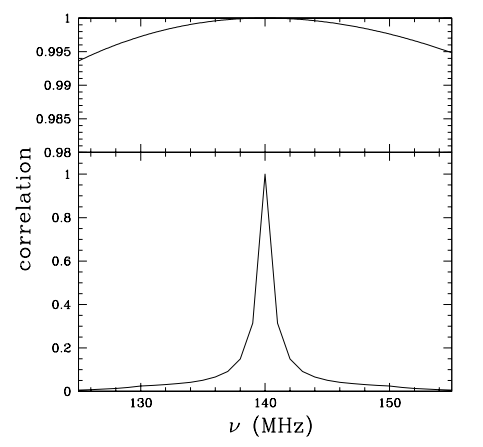
\includegraphics[width=0.4\textwidth]{Chapman_Jelic/Images/santos_freq.png}
\end{center}
    \caption{Left: The 2D power spectrum at 140MHz for the cosmological signal (thick, solid), point sources (thin, solid), Galactic synchrotron (thin, dotted), extra-Galactic free-free (thin, dash), Galactic free-free (thin, long dash) and the CMB (dot-dash). The cosmological signal is dominated by foregrounds at all scales, such that separation based purely on spatial differences in not feasible. Figure taken from Fig. 5 of \cite{Santos2005ApJ...625..575S}. Right: The simulated frequency correlations for the foregrounds (top) and cosmological signal (bottom). This plot shows how the correlation between frequency slices (with the comparison made to a slice at 140 MHz), drops off with increasing frequency separation. The foregrounds are highly frequency coherent, whereas the cosmological signal is significantly less so. Figure taken from Fig. 7 of \cite{Santos2005ApJ...625..575S}.}
    \label{fig:santos_spatial}
\end{figure}

As we have seen in the first half of this chapter, the astrophysical foregrounds are 3-5 magnitudes brighter than the cosmological 21-cm signal and so, by magnitude alone, appear to be the most ominous obstacle to the first detection. Despite, or perhaps because of, their overwhelming magnitude they are well constrained, following power laws with known indices and evolution. The sheer magnitude of the foregrounds means that purely spatial separation, i.e. separation based on only one frequency slice, is not possible: the 21-cm signal and foregrounds are not statistically different enough when only considering spatial scales (see left-hand panel of Fig. \ref{fig:santos_spatial}) \cite{Santos2005ApJ...625..575S,DiMatteo2004MNRAS.355.1053D,Oh2003MNRAS.346..871O,DiMatteo2002ApJ...564..576D}. While separation based purely on spatial scales is not feasible, the high frequency coherence of the foregrounds compared to both the instrumental noise and cosmological signal provides a way to separate out the two signals (foregrounds and both cosmological signal and noise) (see right-hand panel of Fig. \ref{fig:santos_spatial}). 

\cite{Santos2005ApJ...625..575S} and \cite{Zal2004ApJ...608..622Z} exploited the large cross-correlation of the foregrounds in slices at different frequencies to model and remove the foregrounds noting that the frequency coherence was also a useful tool for separation. Polynomial fitting went on to exploit the frequency coherence of the foregrounds across the bandwidth, removing the foregrounds along the line of sight without using any spatial correlation information (e.g. \cite{Bowman2009ApJ...695..183B,Wang2006ApJ...650..529W,Mcquinn2006ApJ...653..815M}. In this method, the foregrounds are modelled by a polynomial function, for example in log-log space such as:

\begin{equation}
\mathrm{\log I} = a_3 +a_2\log\nu + a_1(\log \nu)^2 + ....
\end{equation}

\noindent where $I$ is the brightness temperature of the data, $\nu$ is the frequency of observation and $a_1,a_2,a_3$ are the coefficients which are to be determined in the fit.

Polynomial fitting is a parametric foreground mitigation method. It uses knowledge from simulated foregrounds to tune the coefficients of the polynomial function (e.g. \cite{jelic08}). There are two areas of concern when using this method. Firstly, the effect of the instrument results in a signal which can differ significantly from the frequency-coherent theoretical foreground model (see Section \ref{sec:wedge}). By incorporating weighting according to the amount of information in a particular $uv$ cell, this could possibly be overcome \cite{Liu2009MNRAS.398..401L,Bowman2009ApJ...695..183B}. The second area of concern was that the success of the method relies heavily on having an accurate model for the foreground signal. There are many more instrumental effects than the frequency dependence of the beams, for example polarization leakage (e.g. \cite{Nunhokee2017ApJ...848...47N,Asad2015MNRAS.451.3709A}) and excess instrumental noise \cite{Patil2016MNRAS.463.4317P}. \cite{Wang2013ApJ...763...90W} demonstrated that polynomial removal across the EoR frequency band resulted in significant signal loss when using simulations of complex foregrounds, though they also showed that by fitting a polynomial simultaneously in smaller bandwidth segments this signal loss could be mitigated. Polynomial removal is now rarely used within the interferometric experiments with the exception of the upper limit from GMRT \cite{Paciga2011MNRAS.413.1174P} which used a similar philosophy to remove their foregrounds, albeit by applying a piecewise linear function, as opposed to a polynomial function. 

Aside from interferometric experiments, polynomial fitting does have a prominent place in global EoR experiments (e.g. \cite{Singh2018ApJ...858...54S,Bowman2018Natur.555...67B}) which, due to the coherence of the 21-cm global signal over frequency, means that so far all the more sophisticated methods of foreground mitigation have been unworkable on global simulation and data. For example, the very small number of lines of sight observed by a single global experiment mean that there is not enough spatial information for some non-parametric methods to work.

The Experiment to Detect the Global EoR Signature (EDGES) detection \cite{Bowman2018Natur.555...67B} used a five term polynomial based on the properties of the foregrounds and ionosphere, incorporating the actions of the instrument into their foreground model. The level of accuracy of this method has since questioned however, with the results showing dependence on the description of the foregrounds \cite{Bradley2019ApJ...874..153B,Hills2018Natur.564E..32H}. Overall, polynomial fitting correctly exploits the foreground coherence but it is vulnerable to unknown systematics and unexpected foreground signals. For global experiments there is currently no other option, but for interferometric experiments the methods in the following section provide an alternative.

\subsubsection{Non-parametric foreground removal}
\label{sec:nonpar}
The concern that the instrument might introduce complex spectral structure into the foreground signal has driven research into foreground mitigation methods which rely less on a strongly constrained foreground model. Wp smoothing \cite{Harker2009MNRAS.397.1138H} fits a function along the line of sight whilst penalising the ``Wendepunkt", inflection points, that give the method its name. Unlike polynomial fitting, the function is permitted to be rough but inherently favours the more smooth models. Wp smoothing is applied along each line of sight individually and so spatial correlations of the foregrounds are not utilised in making the foreground fit. The current method employed by the LOFAR EoR pipeline, Gaussian Process Regression (GPR) \cite{Mertens2018MNRAS.478.3640M} also relies purely on spectral information. GPR models the foregrounds, mode mixing components, 21-cm cosmological signal and noise by Gaussian Processes, allowing a clear separation and uncertainty estimation (see Fig. \ref{fig:mertens_comp}). GPR does not require specification of a functional form for each component but instead allows the data to find its own model, while taking into account the covariance structure priors incorporated by the user. This allows a certain level of control, for example splitting the foreground covariance into a smooth intrinsic foreground model and an unsmooth mode mixing component, while still not imposing a strict level of smoothness or a parametric form on the data. 

\begin{figure}
\begin{center}
    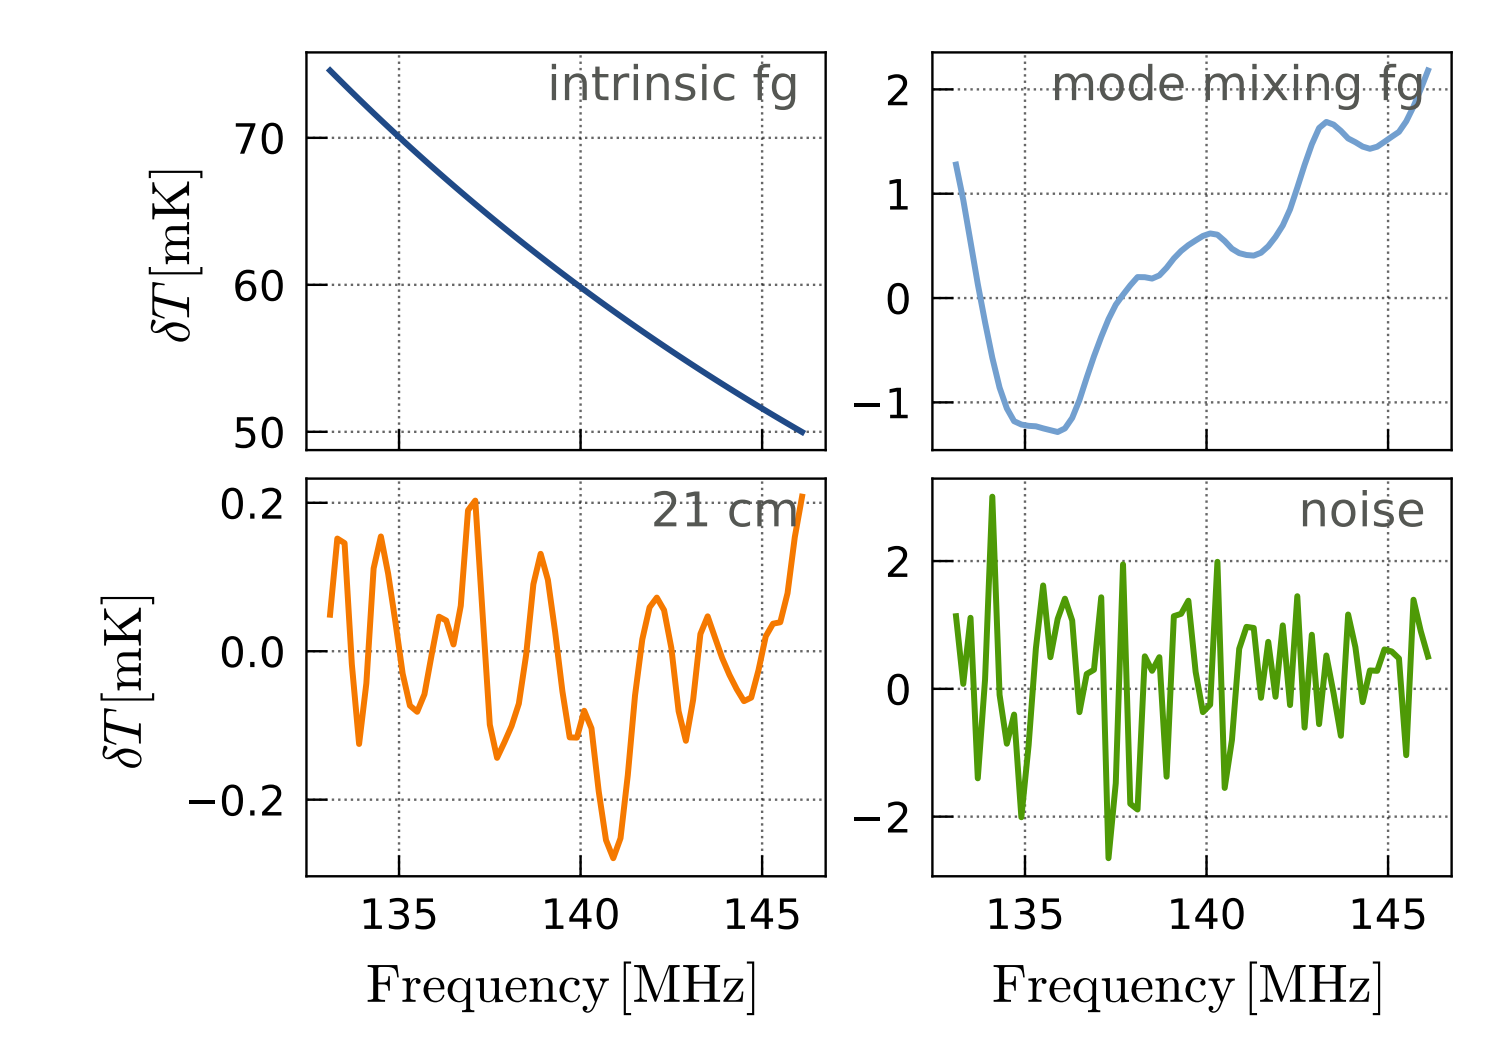
\includegraphics[width=0.9\textwidth]{Chapman_Jelic/Images/mertens_components.png}
\end{center}
    \caption{Simulated components of the observed signal, demonstrating that the smooth foreground signal is accompanied by an unsmooth mode mixing signal. GPR models each of these foreground components separately, making use of prior information about each component in the form of covariance functions. Figure taken from \cite{Mertens2018MNRAS.478.3640M}.}
    \label{fig:mertens_comp}
\end{figure}

 BSS methods have been used in Cosmic Microwave Background experiments \cite{PlanckI2018arXiv180706205P,PlanckIV2018} and their application to EoR data is a natural evolution. BSS methods are used across a wide range of fields in order to separate mixed signals into independent components. The data can be expressed in terms of the mixing model:

\begin{equation}
\mathbf{X} = \mathbf{A}\mathbf{S} + \mathbf{N}
\end{equation}

\noindent where $\mathbf{X}$ is the observed signal, $\mathbf{S}$ are the independent components of that signal, $\mathbf{N}$ is the noise and $\mathbf{A}$ is a matrix determining how the components are mixed, the `mixing matrix'. For an observation of $m$ frequency channels each constituting $t$ pixels and a foreground model of $n$ independent foreground components, the dimensions of these quantities are $\mathbf{X}$[$m$,$t$], $\mathbf{S}$[$n$,$t$], $\mathbf{N}$[$m$,$t$] and $\mathbf{A}$[$m$,$n$].

When this framework is applied to EoR data, the foregrounds are contained within $\mathbf{S}$[$n$,$t$] while the cosmological signal is contained along with the instrumental noise in $\mathbf{N}$[$m$,$t$]. The independent components of the foreground model are not directly related to the Galactic synchrotron, Galactic free-free and extragalactic foregrounds, but instead each independent component is potentially a mixture of all these physical foregrounds. This leaves the user without a physically motivated choice for the number of independent components, so that the number must be chosen empirically based on simulated data. Once a foreground model $\mathbf{A}\mathbf{S}$ has been determined this can then be subtracted from the observed signal, leaving the residual data as with the other methods.

\begin{figure}
\begin{center}
    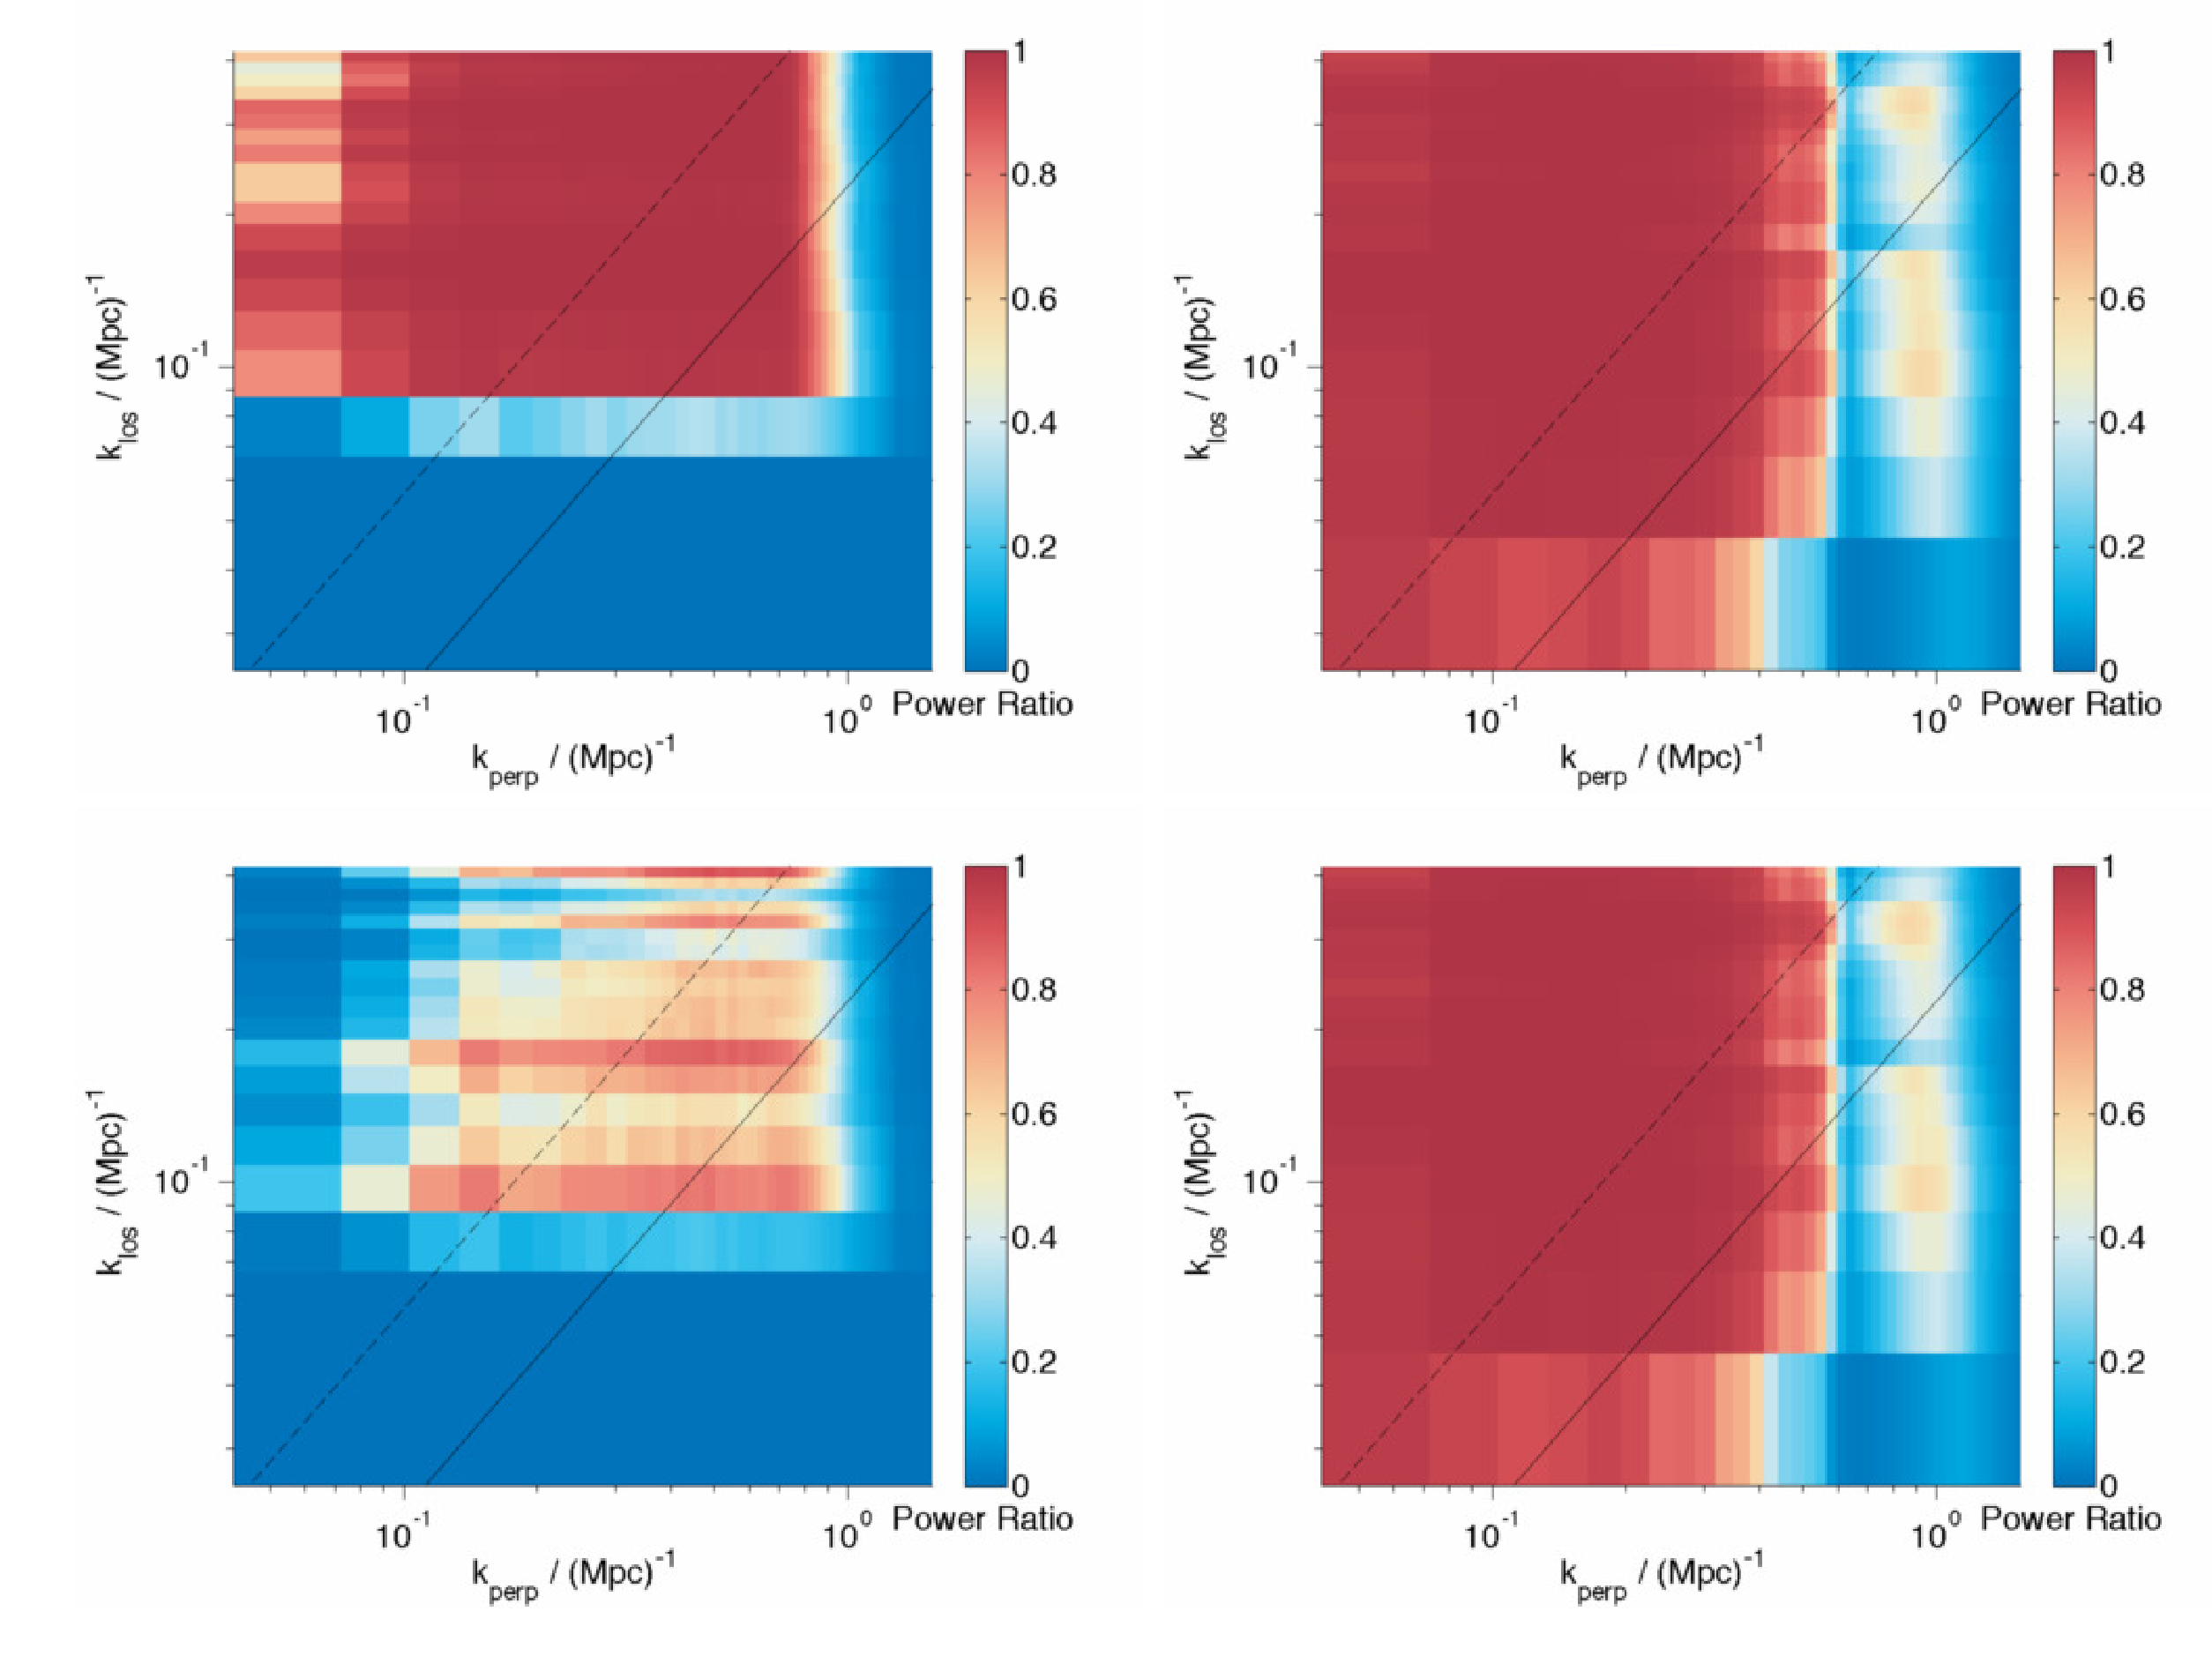
\includegraphics[width=0.9\textwidth]{Chapman_Jelic/Images/Em_window.png}
\end{center}
    \caption{The left column shows the ratio of the simulated components, (cosmological signal / (cosmological signal + foregrounds)), demonstrating that the area of the window free from foreground contamination is small when the foregrounds are unsmooth. The top row is where the foreground model has a random wiggle along the line of sight equal in magnitude to 0.1$\%$ of the foreground signal. The bottom row shows a 1$\%$ wiggle. On the right is the same ratio but with foreground fitting errors after foreground removal by GMCA instead of the simulated foregrounds, demonstrating that the method can open up the EoR window significantly even when the smoothness of the foregrounds is under threat. Figure taken from \cite{Chapman2016MNRAS.458.2928C}.}
    \label{fig:Chap_window}
\end{figure}

The two BSS methods introduced for use on EoR data differ by their definition of independence. FastICA \cite{Chapman2012MNRAS.423.2518C,hyvarinen2004independent,hyvarinen1999fast} is a long-established independent component analysis technique which uses statistical independence to separate out the foreground components. FastICA constrains the different components by maximizing the negentropy of the signal components, utilising central limit theorem which states that the more independent components a signal contains, the more Gaussian the probability distribution function of that signal will be. In contrast, GMCA \cite{Bobin2016AA...591A..50B,bobin2015sparsity,Chapman2013MNRAS.429..165C,Bobin2008StMet...5..307B} is a method developed for use on CMB data that uses morphological diversity to separate out components. GMCA assumes that the data is represented in a sparse manner which can be achieved by a wavelet decomposition. With the independent components unlikely to have the same few non-zero basis coefficients in wavelet space, the method is able to separate out the components according to the differing sparse basis coefficient values. As with FastICA, we actually care little for the independent components individually, it is the combination of those as a whole which form the foreground model, with the method naturally separating out the decoherent noise and cosmological signal. In simulation both these methods have behaved well, opening up the EoR window into the lowest scales even when subjected to unsmooth foreground simulations, Fig. \ref{fig:Chap_window}. GMCA was used to achieve the current LOFAR upper-limit \cite{Patil2017ApJ...838...65P} but since then has not been able to remove the foregrounds down to the same level as, for example, GPR \cite{Mertens2018MNRAS.478.3640M}. The reason for this remains unknown and a full comparative analysis is currently underway. \cite{Mertens2018MNRAS.478.3640M} also expressed concern that because BSS methods are not based on defining the components in a statistical framework relating to the contributions from foregrounds and mode-mixing, they are not easily assessed for uncertainty and physical meaning. The blind methods are very useful as a separate check on results from what are extremely complex experiments, with many unknown unknowns. There is scope to move these methods towards a more parametric framework, perhaps constraining the mixing matrix columns according to the first-hand knowledge about the instrumental effects and foregrounds we have built up from the pathfinder telescopes. This is a similar philosophy as introduced by \cite{Bonaldi2015MNRAS.447.1973B} in Correlated Component Analysis (CCA). While still based on a mixing matrix framework, CCA is a parametric method which constrains the mixing matrix to represent power law behaviour over frequency, fixing the spectral index for a Galactic free-free contribution explicitly. 

While Wp smoothing, GMCA, GPR and FastICA are all labelled non-parametric in the literature, it is important to note than none of them are fully blind or indeed fully non-parametric. Each of them require the selection of parameters to define the fit: whether it is the smoothing parameter in Wp smoothing, or the number of independent components in GMCA and FastICA. So far these parameters have been chosen based on minimizing the foreground fitting error on simulated data, where the foreground model is known. A more robust method is to implement a Bayesian model selection model, as GPR does already. In addition, \cite{Gleser2008MNRAS.391..383G} developed a method based on the Bayesian maximum a posteriori probability (MAP) formalism, assuming priors for the smoothness of the contaminating radiation and for the correlation properties of the cosmological signal and \cite{Zhang2016ApJS..222....3Z} introduced HIEMICA (HI Expectation Maximization Independent Component Analysis), an extension of ICA with a fully Bayesian inference of the foreground power spectra, allowing their separation from the cosmological signal power spectra. Machine learning has also been applied in an effort to seek a foreground model defined by the data itself \cite{Li2019MNRAS.485.2628L}. There are now a multitude of non-parametric foreground subtraction methods available which have each proved their own principle on simulated, and in the case of GPR and GMCA, observed data. Now we know the constraints of the instrument much better, work on the relative advantages and disadvantages of all these approaches are a logical next step.

\subsection{Residual Error Subtraction}
The final stage of foreground mitigation is residual error subtraction \cite{Morales2006ApJ...648..767M,Morales2004ApJ...615....7M}. The residual foreground mitigation errors from the previous two stages (bright source subtraction and diffuse foreground mitigation) produce distinct shapes in the spherical power spectrum, Fig. \ref{fig:ressub}. One can take the spherical power spectrum of the residual data and apply a multi-parameter fit according to the foreground residual and EoR template power spectrum. This allows a final cleaning of residual foreground contamination. \cite{Morales2006ApJ...648..767M} also notes that ``because the residual error subtraction relies on the statistical characteristics of the subtraction errors, the foreground removal steps become tightly linked and we must move from focusing on individual subtraction algorithms to the context of a complete foreground removal framework." This statement leads us neatly to the conclusion of this chapter.

\begin{figure}
\begin{center}
    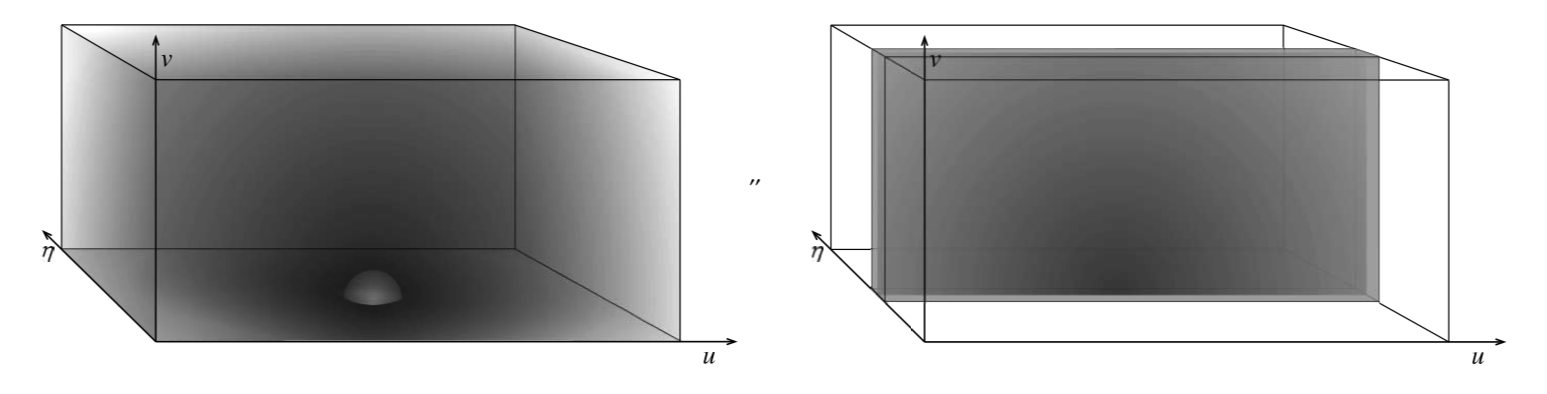
\includegraphics[width=0.9\textwidth]{Chapman_Jelic/Images/res_sub.png}
\end{center}
    \caption{The 3D spherical power spectrum of the EoR signal (left), and an example residual foreground signal template (right), where zero is at the centre of the bottom face of the cuboid. The foreground signal displays a separable-axial symmetry while the EoR signal has a symmetric power spectrum. This contrast allows a further separation stage in order to clean the foreground fitting errors which have accumulated from the previous two stages of bright source subtraction and diffuse foreground mitigation. Figure taken from \cite{Morales2006ApJ...648..767M}.}
    \label{fig:ressub}
\end{figure}

\subsection{Polarisation leakage}\label{sec:leakage}
One of the challenges in calibration is to minimise leakage of polarization signals in total intensity. Otherwise, the polarization leakage can contaminate the cosmological 21-cm signal. 
A level of contamination depends strongly on characteristics of a radio telescope, its calibration strategy, and of polarised emission itself.

Antennas in the low-frequency radio telescopes are dipoles. Dipoles usually come in pairs. In each pair dipoles are orthogonal to each other and each dipole is sensitive to a certain polarisation. Since antennas are also fixed to the ground, it is not possible to preform observations like with the traditional dish-like radio telescopes, where the tracking  is done by steering the dish. Here, the sources are tracked by the beam-forming or simply the observation is done in a drift-scan mode. Depending on the position of the sources in the sky, the sources will see different projections of dipoles. If this geometrical projection  is not corrected during the calibration, or the modelling of and correction for the beam polarisation is not accurate, polarised signals can leak to total intensity and vice versa. 

Since the polarised emission from the Milky Way can have a very complex frequency dependence, a leakage of this signal to the total intensity can contaminate the cosmological 21-cm signal, making extraction and analysis more demanding \cite{jelic10, moore13}. A number of studies addressed this problem for different low-frequency radio telescopes: LOFAR \cite{asad15, asad16, asad18},  MWA \cite{sutinjo15} and PAPER \cite{kohn16}.  Although the assessed polarization leakage in these studies is not limiting current  observations, it will become relevant once we reach a better sensitivity in the data. This will be especially the case for future 21-cm experiments, like HERA and SKA. 

Most of the observed structures appear at Faraday depths $|\Phi|\leq15~{\rm rad~m^{-2}}$, which measures the amount of Faraday rotation by
intervening interstellar medium (see Sec.~\ref{sec:polarfg}). Relatively small Faraday depths indicate polarised emission that fluctuates along frequency on scales  larger than 
the expected cosmological 21-cm signal  in total intensity (e.g. \cite{moore13}). Thus, associated leaked signals can be in principle mitigated, as it was shown in the case of a simple and  thin Faraday screen \cite{geil11}. On the contrary, polarised emission at Faraday depths $|\Phi|\geq15~{\rm rad~m^{-2}}$ can introduce frequency dependent signals, which if leaked can mimic the cosmological signal and make extraction and analysis more demanding (see Fig.~\ref{fig:leakage}).  Prior to the CD/EoR observations, it is therefore important to asses the properties of Galactic polarised emission in desired region in the sky. 

\begin{figure}[!h]
   \centering	
   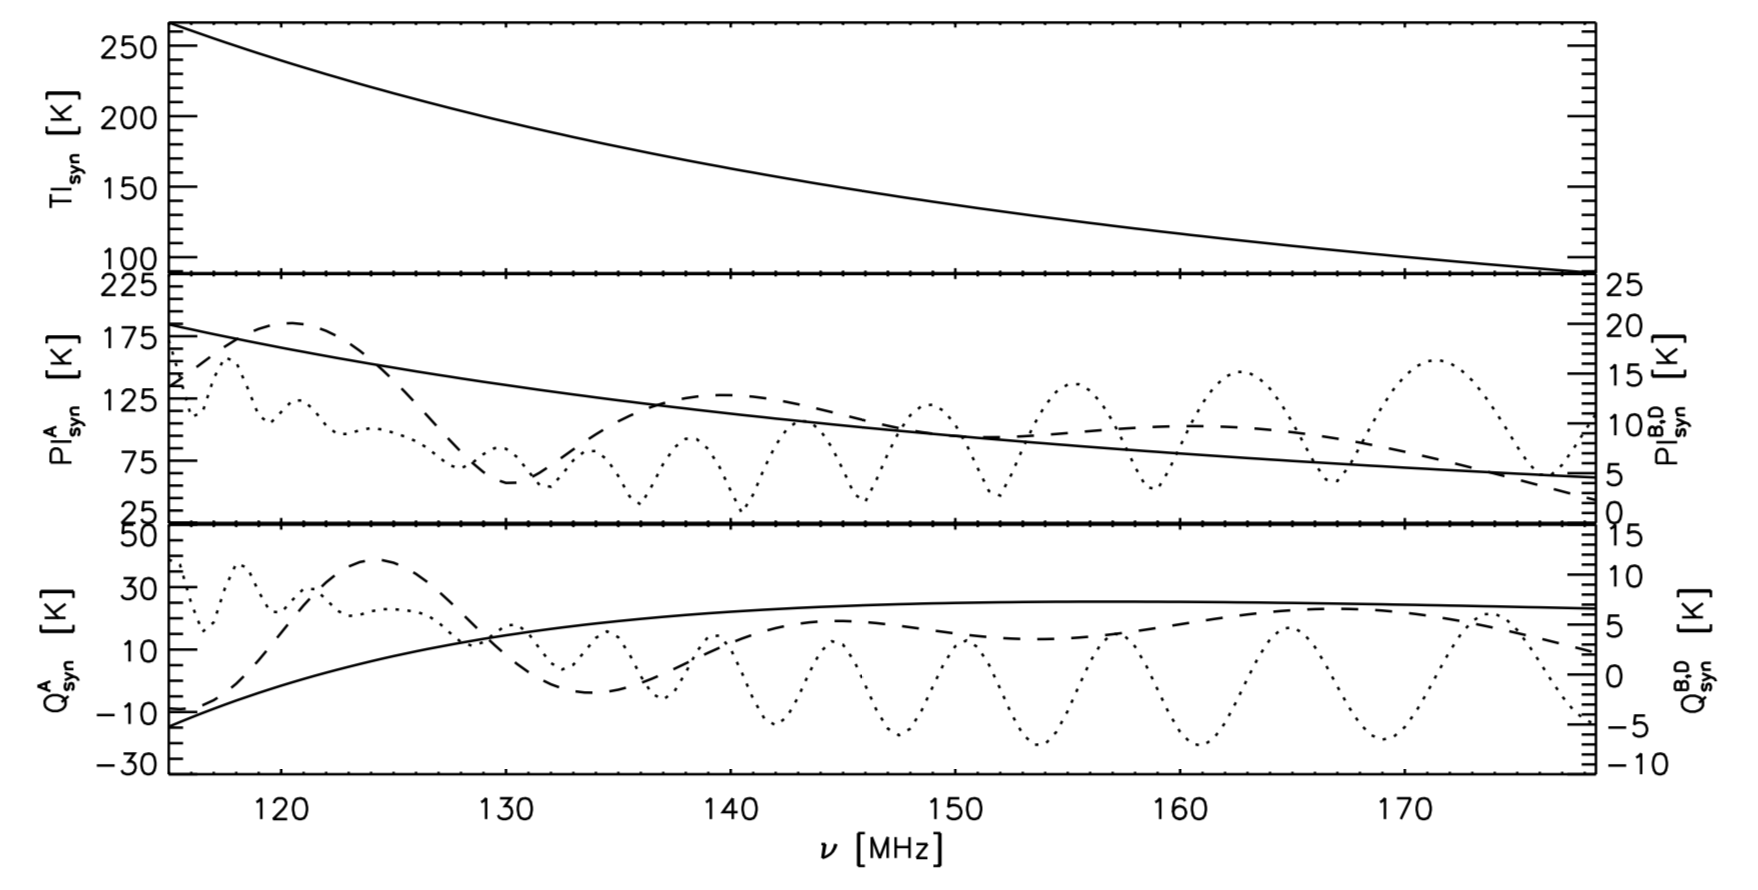
\includegraphics[width=0.9\textwidth]{Chapman_Jelic/Images/leakage.png}
    \caption{How polarisation leakage can contaminate the cosmological 21cm signal: $|\Phi|\leq15~{\rm rad~m^{-2}}$ vs. $|\Phi|\geq15~{\rm rad~m^{-2}}$.}
    \label{fig:leakage}
\end{figure}

\section{Conclusions}
The foreground emission of our Galaxy and extragalactic radio sources dominates over the whole frequency range of the cosmological 21cm experiments. In order to mitigate the foreground emission from the data we need to study and constrain its properties in great details. Thanks to the observations with LOFAR and MWA this is becoming possible.

The current EoR experiments are now modelled and constrained to an excellent degree but during that process there has been a blurring of boundaries between the analysis modules. The calibration stage, once assumed to mitigate foreground point sources only, can erroneously suppress diffuse foregrounds \cite{Patil2016MNRAS.463.4317P} and the mode-mixing of the instrument has required more complex modelling as wide-field effects have become apparent \cite{Thyagarajan2015ApJ...807L..28T}. There are a promising number of foreground mitigation techniques now available providing the necessary diversity of pipelines necessary for verifying the first detection. So far, there has not been a wide-reaching comparison of all of these methods or a complete assessment of their strengths and weaknesses for recovery of the different aspects of the EoR signal such as power spectra or images. Foreground subtraction, suppression and avoidance are now used in combination in the experimental pipelines and the further development of the best combination for these methods will provide an exciting area of research in the next decade.

\bibliographystyle{plain}
\bibliography{Chapman_Jelic/References}


\chapter{Chapter title}

\begin{bf}
  \author{Author Name}\\
  
Abstract\\
\end{bf}

This chapter discusses some important things


\section{A Section}

Lorem ipsum dolor sit amet, consectetur adipiscing elit. Duis eu egestas erat. Maecenas tincidunt lacinia tincidunt. Mauris id lectus nec neque feugiat condimentum vitae at diam. In vel orci nunc, non commodo mauris. Vivamus ipsum enim, vulputate quis pharetra non, molestie quis felis. Vivamus porttitor placerat turpis at accumsan. Nunc tortor velit, faucibus a rhoncus nec, blandit non elit. Nam consectetur lectus eu nisi blandit dapibus rhoncus dui tempus. Mauris fermentum dolor vel ipsum vulputate sit amet ultricies tortor lacinia. Donec ut nibh erat. Morbi nec mi ante. Integer nec vestibulum diam. Donec tincidunt pellentesque quam, ut interdum mauris venenatis condimentum. Nam condimentum, augue in aliquet gravida, neque dui elementum eros, id semper eros purus sed felis. Curabitur in justo sit amet sapien ultrices hendrerit at quis nibh. Quisque iaculis pulvinar tincidunt. 
\begin{eqnarray}
C(12) &= &\left[\overrightarrow{\pi}\cdot\overrightarrow{\phi}(x+r)\right] \nonumber \\ 
&\approx& 1-\mathrm{const}\frac{r^2}{L^2}\int_r^L\frac{x\rmd x}{x^2} + \cdots \nonumber  \\
&\approx& 1-\mathrm{const}\frac{r^2}{L^2}\ln\frac{x\rmd x}{x^2} + \cdots .\label{brokenlongeqn}
\end{eqnarray}

Aenean tellus risus, porta sit amet porta vitae, tincidunt ut felis. Class aptent taciti sociosqu ad litora torquent per conubia nostra, per inceptos himenaeos. Vestibulum ante ipsum primis in faucibus orci luctus et ultrices posuere cubilia Curae; Phasellus pulvinar placerat velit auctor egestas. Vivamus euismod fringilla tincidunt. Sed ut magna felis, id sollicitudin nunc. Quisque a dui eu erat consectetur egestas a quis justo. Aenean euismod congue diam, vel posuere urna fermentum sit amet. Lorem ipsum dolor sit amet, consectetur adipiscing elit. Mauris faucibus lacus eget est mollis auctor. Donec at nibh ligula, et posuere massa. Phasellus quis leo diam \cite{diamantaras1996pcn}.
Donec aliquam blandit risus, eu venenatis ante euismod eu. Curabitur cursus justo id arcu condimentum feugiat. Integer sapien urna, vulputate et adipiscing nec, convallis et justo. Suspendisse in ipsum at felis ornare interdum \cite{tulone2006pts},

\begin{figure}[]
\begin{center}

\includegraphics[width=0.5\textwidth]{Greenhill_Subrahmanyan/01x01-eps-converted-to}
\end{center}
\caption{This is figure 1 in chapter 1.}
\end{figure}

\paragraph{Cras adipiscing} sagittis nunc vel luctus. Suspendisse volutpat augue quis erat semper consequat dignissim tellus euismod. Morbi hendrerit, tellus id aliquam iaculis, nibh leo tincidunt eros, vitae varius ligula felis in mi.

\begin{table}
\caption{Greek Letters.}
\begin{center}
\begin{tabular}{llllllll}
\hline
$\alpha $  & $ \beta $  & $ \gamma $  & $ \delta $  & $ \epsilon $  & $ \varepsilon $  & $ \zeta $  & $ \eta $ \\
 $ \theta $  &  $ \vartheta $  &  $ \gamma $  &  $ \kappa $  &  $ \lambda $  &  $ \mu $  &  $ \nu $  &  $ \xi $ \\
 $ o $  &  $ \pi $  &  $ \varpi $  &  $ \rho $  &  $ \varrho $  &  $ \sigma $  &  $ \varsigma $  &  $$ \\
 $ \tau $  &  $ \upsilon $  &  $ \phi$ &  $ \varphi $  &  $ \chi $  &  $ \psi $  &  $ \omega$  &  $ $ \\
 &  &  &  &  &  &  & \\
$ \Gamma $  & $ \Delta $  & $ \Theta $  &  $ \Lambda $  &  $ \Xi $  &  $ \Pi $  &  $ \Sigma $  & $ \Upsilon $ \\
 $ \Phi$ &  $ \Psi $  &  $ \Omega $  &  &  &  &  &\\
\hline
\end{tabular}
\end{center}\end{table}

\begin{figure}[]
\begin{center}

\includegraphics[width=0.6\textwidth]{Greenhill_Subrahmanyan/01x02}
\end{center}
\caption{This is figure 2 in chapter 1.}
\end{figure}


\bibliographystyle{plain}
\bibliography{Greenhill_Subrahmanyan/References}



\chapter{Status of 21~cm interferometric experiments}

\begin{bf}
  \author{Cathryn M. Trott (ICRAR-Curtin), Jonathan Pober (Brown University)}\\

Abstract\\

Interferometric experiments of the reionization era offer the advantages of measuring power in spatial modes with increased sensitivity afforded by multiple independent sky measurements. Here we review early work to measure this signal, current experiments, and future opportunities, highlighting the lessons learned along the way that have shaped the research field and experimental design. In particular, this chapter discusses the history, progress, challenges and forecasts for detection and exploration of the spatial structure of the 21~cm brightness temperature signal in the Epoch of Reionisation using interferometric experiments. We discuss GMRT, PAPER, LOFAR, MWA, and the future HERA and SKA.
\end{bf}

\section{Introduction}
%Some rehash of the abstract with some extra guff. Include list of experiments with references.

Because they provide both rapid mapping speed and good angular resolution, interferometers have become the preferred instrument for experiments looking to measure the expected spatial fluctuations in the 21~cm signal. 
The current instruments hosting such experiments include the Murchison Widefield Array, MWA{\footnote[1]{http://www.mwatelescope.org}} \cite{bowman13_mwascience,tingay13_mwasystem,jacobs16}; the Precision Array for Probing the Epoch of Reionization, PAPER{\footnote[2]{http://eor.berkeley.edu}} \cite{parsons10}; the LOw Frequency ARray, LOFAR{\footnote[3]{http://www.lofar.org}} \cite{vanhaarlem13,patil16}; and the Long Wavelength Array, LWA{\footnote[4]{http://lwa.unm.edu}} \cite{ellingson09}. In the future, we expect the Hydrogen Epoch Reionization Array, HERA \cite{deboer16} and the Square Kilometre Array, SKA-Low \cite{koopmans15}.
Sensitivity predictions for most of the current experiments (e.g. \cite{beardsley13,pober14}) find that they will not be capable of achieving the necessary signal-to-noise to image the 21~cm signal directly (although see \cite{2012MNRAS.425.2964Z} for a study with LOFAR).  As such, most of these experiments are targeting a detection of the 21~cm power spectrum, which can be constrained with higher signal-to-noise compared with an image because the isotropy and homogeneity of the Universe allows the 3D $k$-space power spectrum to be averaged over spherical shells of constant $|k|$.  
% \jp{It's not clear to me what kind of opportunity we'll get to see and reference chapters by other authors, or whether we're just supposed to be completely self-contained.  But this seems like something that would be described in Gianni's chapter.} \cmt{Yes, I was conscious of this potential overlap. I will await feedback from the other authors on this, but I think we can mention concepts to ensure ours is self-contained.}
Even using the power spectrum, typical predictions for the requisite observing time are of order 1,000 hours (see Figure \ref{fig:current}).  

However, beyond the need to achieve the requisite sensitivity, experiments are faced with the daunting task of isolating the 21~cm signal from foregrounds that can be up to five orders of magnitude brighter.  While the two can, in principle, be separated by their distinct spectral behavior, the inherently frequency-dependent response of radio interferometers complicates the picture significantly.  In this chapter, we review the challenges faced by current interferometric 21~cm experiments as well as the progress to-date in overcoming them.  The detailed structure of this chapter is as follows.  In \S\ref{sec:early_work}, we present the history of experiments and techniques that led to the design of current 21~cm experiments.  In \S\ref{sec:methodologies}, we discuss the distinct approaches each experiment has developed to overcome the challenges associated with these observations, and in \S\ref{sec:results} we review the current published upper limits on the 21~cm signal strength from these experiments.  In \S\ref{sec:challenges}, we highlight the currently unsolved problems at the forefront of experimental 21~cm cosmology and conclude in \S\ref{sec:prospects} with a discussion of the potential for both current and future experiments to overcome them.

\section{Early work}
\label{sec:early_work}
The origins of the approaches that current experiments are taking to detect the Epoch of Reionization power spectrum can be traced to the development of radio interferometry observational techniques and Cosmic Microwave Background (CMB) analysis methodology.

Radio interferometers measure the cross-correlation of voltages detected with two antennas, extracting the sky signal in a complex-valued dataset that encodes sky emission location and intensity, and as a function of antenna separation vector and frequency \cite{tms}. For small field-of-view instruments (large antenna aperture), the measured signal is well-approximated as the 2D Fourier Transform of the sky brightness, attenuated by the antenna response function (the primary beam).

Motivated by analysis of CMB datasets in the 1990s and 2000s, and the curved nature of full-sky imaging, early discussion of power spectrum estimators used spherical harmonic basis functions to describe the signal and extract optimal estimators \cite{tegmark97}. CMB studies suffer from some of the challenges faced also by EoR experiments: wide fields-of-view, low sensitivity, limited angular resolution, and foreground contamination. Unlike EoR, which is an evolving signal in redshift space, CMB studies are single frequency experiments focussed on angular statistics. As such, the foreground mitigation and treatment approaches of CMB studies are of limited use for EoR studies, which attempt to separate foregrounds from the 21~cm signal using the frequency axis. Nonetheless, the fundamental need to extract a weak signal from complex and highly-contaminated data is shared between the two fields, and Tegmark used this experience to apply CMB analysis techniques to early EoR methodology development. 
Since an interferometer natively measures in Fourier space, there was a transition from the natural basis of curved sky functions (spherical harmonics) to the interferometer measurement space (Fourier modes) in discussion of optimal estimators for EoR science \cite{liu11}.

This work was supported by groundwork laid out for doing EoR power spectra with radio interferometers, including cosmological and unit conversions \cite{morales04,parsons10} and noise considerations for astrophysical parameter estimation with specific future experiments \cite{mcquinn06}. McQuinn and colleagues discussed a simple foreground model where fitting of a smooth spectral function could remove their effect cleanly, focussing on array sensitivity as the limiting factor for future experiments. 
%JCP: Who is "they"?  Is it a Bowman paper you're referencing?  The Morales 04 paper of the above paragraph? RESOLVED
However, the lack of any real-world experiments attempting the detection meant they failed to realise the extent of foreground spectral contamination.

More sophisticated approaches to foreground modelling and mitigation appeared in the mid-2000s, with \cite{2009ApJ...695..183B} beginning a set of papers that explored the signature of smooth spectrum sources in the EoR power spectrum parameter space. Initially, low-order polynomials were explored to fit and remove these sources. However, lacking a physical motivation for this functional form to robustly separate foregrounds from cosmological signal, polynomials  were replaced with more realistic functions. Ultimately, the likelihood of removing not only foregrounds but also cosmological signal when fitting and subtracting models, particularly considering the large difference in magnitude of the two signals, has steered the research field away from this approach to foreground mitigation.

As part of this better appreciation for the impact of foregrounds, particularly with the knowledge that they are used also for data calibration, \cite{datta10} explored the required accuracy of source models such that foregrounds may be subtracted to a level sufficient to detect the EoR. This work was the first to show the characteristic wedge in power spectrum parameter space, a triangular region in angular and line-of-sight wavenumber space representing the signature of smooth-spectrum sources observed with an interferometer.

\section{Experimental methodologies and current experiments}
\label{sec:methodologies}
In this section we introduce the different instruments that have previously taken, or currently are taking and analysing, data for an interferometric EoR experiment. We start by presenting the relevant parameters of the telescopes that these experiments use, highlighting and motivating the different observational and analysis approaches taken by each. Table \ref{table:parameters} lists the location (including latitude), frequency (redshift) range, number of stations/antennas, station diameters, and maximum baseline, and field-of-view at 150\, MHz for the relevant instruments. Italicised telescopes are discussed in this Chapter. We also plot the full uncertainties (including sample variance) for a 1000~hour observation at $z$=8.5 (10~MHz bandwidth) for each experiment as a function of spatial wavenumber in Figure \ref{fig:current}. We uniformly assume that the modes within the horizon are inaccessible due to foreground contamination, and note that this is a broad assumption that is not applicable to all experiments. Note also that MWA's and HERA's large fields-of-view gives them access to smaller wavenumbers. This figure also includes a nominal signal strength (black, 21cmFAST, \cite{mesinger11}), but this level is highly uncertain. The proximity of the curves to this line highlights the difficulty with predicting the real sensitivity of experiments, particularly in light of the large number of observing hours required to reach an expected detection.
\begin{table}[ht]
\centering
\begin{tabular}{|c||c|c|c|c|c|}
\hline 
Facility & Location (Latitude) & Freq. [MHz] ($z$) & $N_{\rm ant}$ & Max. baseline & FOV$_{150}$ \\
\hline
\textit{GMRT} & India (19.1$^{o}$N) & 150--300 (3.7--8.5) & 30 & 30~km & 2.5$^{o}$\\
\textit{MWA} & Australia (26.5$^{o}$S) & 70--90, 135--195 (15--19, 6--10) & 128 & 5~km & 25$^{o}$\\
\textit{LOFAR} & Netherlands (52.9$^{o}$N) & 30--80, 120--190 (17--46, 6--11) & 50--60 & 50~km & 5$^{o}$\\
\textit{PAPER} & South Africa (30.6$^{o}$S) & 110--180 (7--12) & 32--64 & 210~m & 60$^{o}$\\
LEDA\footnote[1]{} & USA (34$^{o}$N) & 45--88 (15--30) & 256+ & $<$10~km & 70$^{o}$\\
21CMA & China (42$^{o}$N) & 50--200 (6--27) & 81 & 6~km & 10$^{o}$\\
\hline \hline
\end{tabular}
\label{table:parameters}
\caption{General parameters for the telescopes undertaking interferometric observations of the Cosmic Dawn and EoR. Italicised telescopes are discussed in this Chapter. $^1$LEDA is a total power experiment using interferometry for data calibration.}
\end{table}
\begin{figure}[ht]
\centering
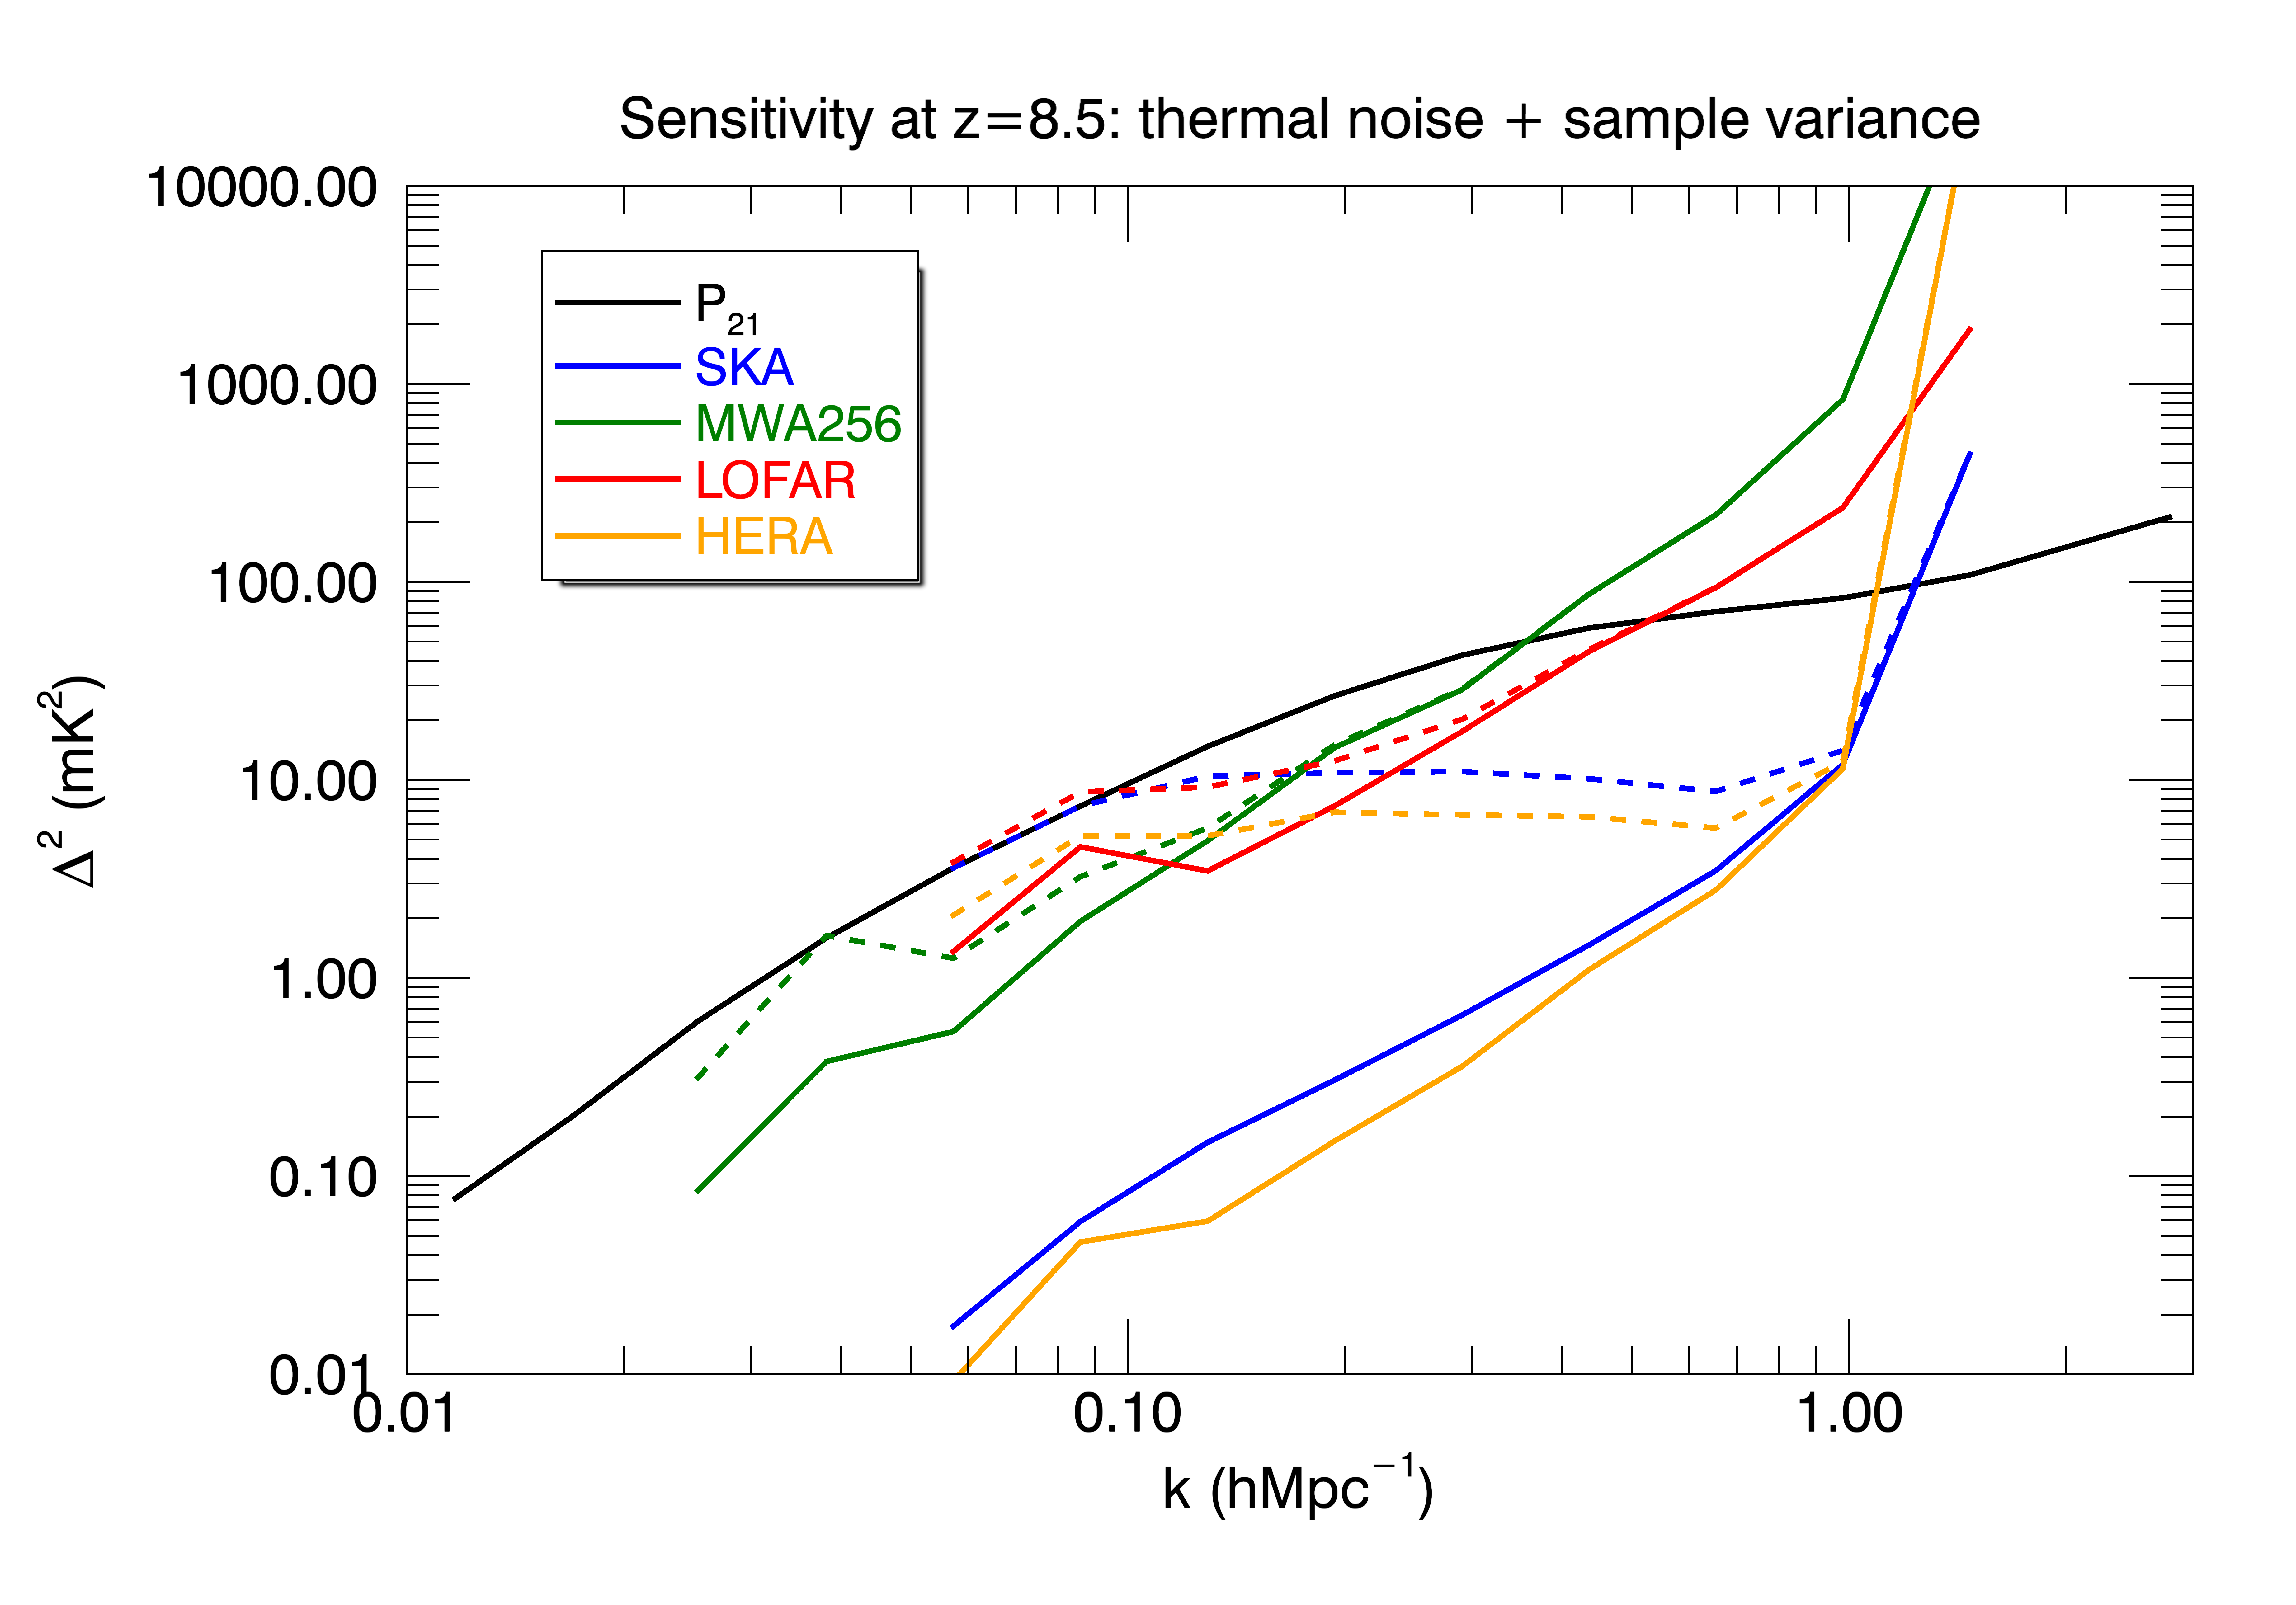
\includegraphics[width=1.0\textwidth]{Trott_Pober/sensitivity_horizoncut.png}
\caption{Estimated total uncertainty on the dimensionless power spectrum for a 1000 hour observation with several experiments at $z$=8.5 compared with a model input power spectrum (21cmFAST,\cite{mesinger11}), and assuming that modes within the horizon are inaccessible. Solid lines are only thermal noise uncertainty, while dashed lines include sample variance. (Black) Model cosmological signal; (blue) SKA; (green) MWA256; (red) LOFAR; (orange) HERA.}\label{fig:current}
\end{figure}
%JCP: If it's not too hard, a color legend on the figure would be welcome. Done!
The parameters shown in the table, and the curves shown in Figure \ref{fig:current} motivate and frame the discussion of different experiments in the following sections. Experiments are forced to undertake different approaches to observations and data analysis, because the physical limitations of the systems promote different systematic errors into the forefront for each experiment. There is no silver bullet telescope for undertaking this experiment, however, and after reviewing the main experiments, we discuss the pros and cons of different features.

\subsection{Giant Metrewave Radio Telescope - GMRT}
\label{sec:gmrt}
The GMRT \cite{swarup91} is a Y-shaped array of 30 45~m dishes spread over 25~km in western India. Operating between 50~MHz and 1420~MHz, its 153~MHz receiver has been most used for Reionization studies. Motivated by early work in the post-reionization era (325~MHz and 610~MHz receivers) to statistically detect 21~cm fluctuations and understand the foreground contamination to these data, the low frequency receiver opens the door to exploring the Reionization era. The methodology developed has focused on angular power spectra, measured at a range of frequencies, and pioneered much of the early work to use spectral correlation of foregrounds as a way of treating them. With a lack of short baselines and poor instantaneous $uv$-coverage (Figure \ref{fig:gmrt}), the array is suited to building high resolution foreground models, and computing the foreground angular correlation function (\cite{rana19}).

GMRT work has largely utilised the visibility correlation function, which cross-correlates visibilities to study the spectral and spatial structure of the sky. Visibility correlation functions were also explored for 21CMA analysis \cite{zheng12}. Unlike other experiments, which have cross-correlated interleaved time samples to remove noise power bias, GMRT has usually opted for cross-correlating visibilities from adjacent frequency channels. This has different systematics, with finer spectral resolution required to minimise visibility decorrelation.

During the 2000s, there was a series of papers developing a formalism for use of this visibility correlation function to measure angular modes.
\cite{bharadwaj01} introduced a cross-visibility angular correlation function to measure HI fluctuations post-reionization. 
%First use of cross-correlating different frequency channels to remove noise bias.
%JCP: I think the above sentence (now commented) was basically said in the previous paragraph?
\cite{bharadwaj05} then related the cross-visibility correlation function across baselines and frequencies to the power spectrum of brightness temperature fluctuations, presenting the full formalism and expected results in different epochs. They suggest that the cosmological is uncorrelated for frequency channel differences larger than 1~MHz, allowing signal to be `easily distinguished from the continuum sources of contamination'.
\cite{ali08} then extended this formalism to model the expected foreground continuum signatures in the cross-correlation visibility space, and compared with GMRT observations. Their results were hindered by calibration errors, which caused decorrelation of the signal over frequency, but presented the first application of this technique to data.
\cite{datta07} provided an extension of the visibility cross-correlation approach to estimating power spectra to a multi-frequency angular power spectrum (MAPS), utilising decorrelation of signals over frequency to extract information about bubble sizes and distributions as a function of redshift while suppressing the effects of foreground contamination.
%JCP: These are all important papers, but this paragraph is tough to get through -- in part because the GMRT analysis framework has been so incrementally built up over the years.  Not sure if there's much to do about it, but thought I'd mention it.

\cite{ghosh11} published the first measurement of post-reionization neutral hydrogen fluctuations with GMRT (HI intensity mapping) at $z$=1.32 (610 MHz) and using the MAPS formalism. 
%JCP: First mention of MAPS -- I think it's from one of the papers in the previous paragraph, but not sure which one?
They used a fourth-order polynomial to remove smooth foregrounds, in line with early attempts with many experiments to fit a parametric function without physical motivation.
\cite{ghosh11a} then demonstrated improved foreground removal for 610 MHz observations by tapering the primary beam function and reducing sidelobes; 
\cite{ghosh12} further extended the work to the reionization epoch using 150 MHz observations to characterize the foregrounds with the MAPS formalism.

Using an alternative analysis to the MAPS formalism, \cite{paciga11} analysed 50h of data at $z$=8.6 with a simple piecewise linear foreground subtraction method and cross-correlation of foreground-subtracted images.  The result was a reported upper limit on the 21~cm signal strength of (70 mK)$^2$.
However, \cite{paciga13} re-analysed the data with a more sophisticated foreground subtraction technique, including a calculation of signal loss due to foreground fitting. The result was an increase in the upper limit to (248 mK)$^2$, indicative of the degree to which signal loss can affect results.

More recently, \cite{chouduri14} published a series of papers introducing and exploring the use of two new optimised power spectrum estimators using visibility correlations: the Tapered Gridded Estimator (TGE) and Bare Estimator (BE). The key concept for the TGE, which has been further discussed in the literature in subsequent papers \cite{2016MNRAS.463.4093C}, is to use a Fourier beam gridding kernel that is larger than the physical beam kernel, thereby decorrelating sources at the edge of the field-of-view. 
%JCP: Unsure about the phrase "which has been further discussed in the literature" -- we should either omit or give references.
Note that this approach is not a silver bullet to removing the effect of horizon sources, because their sidelobes remain in the data even if they have been attenuated. Originally developed as angular power spectra as a function of frequency, the TGE work has recently been expanded to use the line-of-sight spatial information \cite{bharadwaj19}. The BE directly squares adjacent visibilities to provide individual measurements of the power, but this has not been used further, possibly due to the large number of visibilities that are accumulated and stored.
%JCP: Anything to say about the BE?

Additionally to power spectra, \cite{ali06} predicted the amplitude of a bispectrum signal with GMRT using its shortest baselines by modelling non-linear clustering. They predicted the signal strength to be comparable to the power spectrum and detectable in 100 hours but this project has not been explored observationally with this instrument.
\begin{figure}[ht]
\centering
\includegraphics[width=0.85\textwidth]{Trott_Pober/gmrt_array.png}
\caption{Array configuration for the GMRT: thirty 45~m dishes spread over 30~km.}\label{fig:gmrt}
\end{figure}


\subsection{Murchison Widefield Array - MWA}
The Murchison Widefield Array (MWA) is a 256-element interferometer in the Western Australian desert. In Phase I of the array, operating from 2013--2016, it was composed of 128 tiles of 16 dual-polarization dipoles, spread over 3~km \cite{tingay13_mwasystem}. Phase II (2016--) expanded the array to 256 tiles, with longer baselines for improved survey science and sky model building (5~km), and two hexagonal sub-arrays of 36 tiles with short spacings available for redundant calibration and improved EoR sensitivity \cite{wayth18}. It operates in two distinct modes: Extended Array (128 tiles with long baselines), and Compact Array (128 tiles with short baselines including two 36-tile redundant subarrays in a hexagonal configuration). The Compact Array is principally used for EoR science (see Figure \ref{fig:mwa}).
%JCP: I was going to add some text about how Phase II operates in extended and compact modes, but then noticed Figure 3 only has an image of the extended array.  Is there a reason for the omission?
The MWA is a general science telescope, with multiple science goals \cite{bowman13_mwascience}. As such, it balances high surface brightness sensitivity on EoR scales, redundant and non-redundant elements, and longer baselines for good imaging capabilities. The instantaneous $uv$-coverage of the MWA is excellent, allowing for science-quality snapshot imaging (2-minute). The MWA is also a wide-field instrument, with a field-of-view of 25~degrees at 150~MHz. This wide field-of-view, combined with the complex frequency-dependent shape of the aperture array primary beam, and analogue electronics, create challenges for data analysis. The two-stage analogue beamformer produces a frequency bandpass that contains 24 coarse channels over a 30.72~MHz bandwidth (chosen from the full bandwidth listed in Table \ref{table:parameters}), with missing regular channels between the coarse bands. This instrumental spectral structure provides a challenge to producing instrumentally-clean output EoR datasets.
\begin{figure}[ht]
\centering
\includegraphics[width=0.42\textwidth]{Trott_Pober/mwa_128_array.png}
\includegraphics[width=0.52\textwidth]{Trott_Pober/MWA_PhaseII_pos.png}
\caption{Array configurations for the MWA (Phase I, left; Phase II, right, including cutout of hexagonal subarrays (blue)): 128 (256) 4.4~m aperture array tiles spread over 3 (5)~km.}\label{fig:mwa}
\end{figure}

Early deployments of the array, with 32 tiles, were used for preliminary science, and to begin to survey the EoR fields \cite{2012ApJ...755...47W}. Upon completion of the 128 tiles, the MWA Commissioning Survey provided the first sky catalogue for use for calibration of EoR data \cite{2014PASA...31...45H}. This work paved the way for the GLEAM survey \cite{wayth15} and catalogue \cite{hurleywalker16}, yielding 300,000 sources in the southern sky. GLEAM provides the basis for the current sky model for point sources in EoR observations, augmented by individual models for extended sources.

%JCP: Note, I moved this paragraph up one in order, as I think it flows better.
In line with developments in concurrent experiments, prior to data acquisition the MWA EoR collaboration focused on relatively simplistic foreground fitting and removal methods, but with an increasing understanding of the signature of smooth-spectrum foregrounds in the wavenumber parameter space of an interferometer \cite{2009ApJ...695..183B,datta10,trott12}. 
%JCP: Not entirely clear what you mean by the second half of this sentence.
%JCP: These next sentences are fairly redundant with things you said at the beginning of this section, but perhaps more clearly worded -- so you can maybe swap text as you see fit?
%It also concentrated efforts on building an instrument with hybrid capabilities of high surface-brightness sensitivity and short baselines for EoR, and longer baselines for survey science and calibration model building \cite{tingay13_mwasystem}. Like LOFAR and GMRT, but unlike PAPER, the MWA is a general science telescope with EoR being one of the primary science pursuits \cite{bowman13_mwascience}.
There are now two primary EoR data calibration and source subtraction pipelines used by the collaboration: the Real-Time System (RTS, \cite{mitchell08}) and Fast Holographic Deconvolution (FHD, \cite{2012ApJ...759...17S}). Both use underlying catalogues of sources that have been generated by cross-matching multiple low-frequency sky catalogues. PUMA \cite{line17} generates an observation-specific sky model of point sources and double sources \cite{procopio15}, and includes shapelet-based and point source-based models for extended sources. The RTS calibrates the data in two steps, both of which rely on a weighted least-squares minimisation: (1) overall direction-independent (flux density and phase) calibration on a full model of 5,000 sources; (2) direction-dependent corrections along the line-of-sight to bright sources. The direction dependent corrections are then applied to sources in the region of the fit, and the 5,000 source sky model is subtracted.
FHD calibration \cite{2012ApJ...759...17S} computationally optimizes the direction-dependent and wide-field imaging steps by pre-computing the mapping from Fourier to real space. FHD relies on an underlying point source sky model \cite{2016MNRAS.461.4151C}, which generates an observation-specific calibration model for $>$10,000 sources based on the GLEAM catalogue and other cross-matched surveys.

Early developments of power spectrum pipelines stemmed from the inverse covariance quadratic estimator framework pioneered in CMB studies \cite{tegmark97}, and applied to theoretical EoR datasets by Liu \& Tegmark in 2011 \cite{liu11}. This work was further developed by Dillon in a series of papers that explored how to bridge some of the differences between the ideal estimator and a physical dataset \cite{dillon15,dillon13}. In particular, Dillon discussed missing data, and large data volumes. An adapted approach was then applied to three hours of MWA data, showing promising results \cite{dillon13}. 

One key feature of the optimal quadratic estimator formalism is the whitening of data according to the correlated covariance introduced by the uncertainty on residual foregrounds. This is effectively a down-weighting of data that are heavily affected by foregrounds, thereby improving signal-to-error. Subsequent analysis of a higher redshift dataset was used to estimate the principal eigenmodes of the data in spectral space, identifying these with bright foregrounds \cite{dillon15}. 
%JCP: Just going off memory here, but I thought Dillon tried to estimate the eigenmodes using an annulus of |u| excluding the (u,v) cell containing the actual data being weighted -- to try and avoid the re-substitution bias.  This was the suggestion of an astute reviewer, so it didn't appear in the first draft. %CMT Yes, I see that now in the paper. I will amend this.
The covariances of these modes were then used in the estimator to down-weight and decorrelate data, yielding improved limits at $z=6.8$. However, as with commensurate and subsequent work with PAPER that used this technique, it had the large potential to cause bias in the estimates. Re-use of the same dataset to empirically estimate the data covariance, and then fit for it, causes re-substitution bias, a well-known statistical effect where the performance of an estimator can appear much better than it actually is. In this work, Dillon was careful to estimate covariances empirically while omitting the $uv$ cells in question, to avoid bias, however there was still limited information available in the remaining cells. Thus, although this work was careful to not try to subtract the foreground bias directly, use of the empirical covariance in the data weighting, and lack of a full end-to-end simulation to demonstrate no signal loss, makes this approach prone to large bias.  It has not been used to analyze MWA data since the original analysis in \cite{dillon15}.

In a later paper, describing the CHIPS estimator, Trott also developed an inverse covariance quadratic estimator formalism using a model foreground covariance \cite{trottchips2016}. Unlike the empirical approach of earlier work, this does not use the data itself to form the foreground covariance, but a model for the expected spatial and spectral structure of point source foregrounds. However this approach can suffer from similar effects, whereby error in the covariance can propagate into the analysis. Therefore, this inverse foreground covariance has never been applied to data used in publication due to the output's sensitivity to the choice of foreground model.

A second principal power spectrum estimator for MWA EoR analysis, $\epsilon$ppsilon, was independently developed from CHIPS \cite{barry19}. $\epsilon$ppsilon prioritizes the propagation of thermal noise error from the visibilities (with estimates provided by FHD) through to the power spectrum while also providing a suite of diagnostics for assessing the performance of the estimator in a number of domains.  

Both $\epsilon$ppsilon and CHIPS (without the foreground covariance weighting) were used in the EoR limit paper led by Beardsley \cite{beardsley16}, which processed 32~hours of MWA Phase I high-band data to power spectrum limits. 
At the time, these results were highly-competitive in the field, but the data were clearly still systematic-dominated. At a similar time, Ewall-Wice published the first measurement of upper limit from the Cosmic Dawn (Epoch of X-ray heating, EoX) from 3-hours of MWA data above $z=15$ \cite{ewall-wice16}.

One of the clear outcomes of the early upper limit publications from MWA (and other instruments, particularly LOFAR) was that the data were highly systematic-dominated in modes relevant for EoR, and accumulating more data into the power spectrum estimator would offer no advantage. With this realisation, the MWA collaboration embarked on a two year program to prioritize understanding and treating systematics over processing large datasets, despite more than a thousand hours having been collected by the instrument. This work encompassed (1) improving the sky model (point, extended and multiple sources, \cite{procopio15,trottwayth17_extended}); (2) understanding the impact of calibration choices on residuals and uncertainties \cite{barry16,trottwayth2016,trott17_skala,ewall-wice17,murray17}; (3) improving the primary beam modelling \cite{line18}; (4) developing data quality metrics for data triaging (RFI, ionospheric activity, \cite{jordan16,trott18,wilensky19}), (5) developing and refining redundant and hybrid calibration pipelines for Phase II \cite{li18_redundant,joseph18,byrne19}. A final important step was the development of a full end-to-end simulation to demonstrate that there was no signal loss in the chain from telescope to data product. The results of this work include upcoming EoR limits from re-analysis of Phase I data and new Phase II data, as well as exploration of new techniques for exploring the EoR \cite{trott19_bispectrum}.
%JCP: Nichole's paper probably won't be published on 6/21, but may be by the end of July.  We should consider mentioning this to Andrei and saying we might want to update this section last minute.

A final, key insight from recent work helps to address the current questions in the EoR research field about robustness of any future claimed detection of cosmological signal. Along with confirmation by other telescopes, ability to detect the same signal in independent observing fields, where the foregrounds are different, is crucial. In \cite{trott19_kde}, MWA data from two observing fields was studied with a Kernel Density Estimator to understand the similarities and differences between the statistical structure of data from independent sky areas. This work can lead to a better understanding of robustly discriminating contamination from cosmological signal.


\subsection{Low Frequency Array  - LOFAR}
LOFAR is a composite aperture array low-frequency radio interferometer. It has two primary station types; the High-Band Antennas (HBA, 120--190~MHz) and Low-Band Antennas (LBA, 30--90~MHz). Both station types have been used for EoR and Cosmic Dawn science. Athough LOFAR formally contains baselines of thousands of kilometres to the international stations, it is only the Dutch-based stations that are used for actual EoR measurements. Figure \ref{fig:lofar} shows the central stations (blue cut out) and the nearest remote stations (red).
\begin{figure}[ht]
\centering
\includegraphics[width=0.85\textwidth]{Trott_Pober/lofar.png}
\caption{Array configuration for the central and inner remote stations of LOFAR (red), and subplot showing the central stations only (blue): 30--40~m aperture array dipole stations spread over tens of kilometres.}\label{fig:lofar}
\end{figure}

The LOFAR latitude allows for circumpolar observations with long winter nights. As such, one of the primary observing fields is the North Celestial Pole, which can be observed for more than 12 hours in the winter months.
Early work with the LOFAR EoR Key Science Project focussed on foreground mitigation, choice of observing fields, and data analysis methodology. As with many of the published papers in this early epoch, foregrounds in \cite{2008MNRAS.389.1319J} were modelled to be subtracted with a simple smooth fitting function. This work is notable because it provided realistic models for a range of different foreground components, and included discussion of the treatment of polarized foregrounds.

\cite{2010MNRAS.409.1647J} extended the work from 2008 to focus on simulations of Faraday Rotation from polarized Galactic foregrounds. FR rotates the phase of the intrinsically-smooth foreground component yielding spectral structure that may mimic the EoR signal. In this work, Jeli{\'c} shows the effect of inaccurate data calibration on polarized emission, which can imprint total intensity structure if the polarized instrumental response is incorrect.

%In 2008, a landmark study published by \cite{2008MNRAS.389.1319J} explored realistic resolved and unresolved foregrounds for the LOFAR experiment. This work set the scene for more complete and realistic models of the true spatially- and spectrally-varying foreground sky. It was later extended to include polarized foregrounds \cite{2010MNRAS.409.1647J}.
%JCP: This last paragraph seems both out of place and an abrupt end to the section.  Do you want to do more with it?  It also seems to be discussed in the LOFAR section itself, so perhaps it could be omitted.

The SAGE algorithm (Space Alternating Generalized Expectation Maximization) was first introduced in 2011 by \cite{2011MNRAS.414.1656K}, and provides the basis for all calibration of LOFAR EoR datasets to the present day. Based on the well-known Expectation Maximization (EM) algorithm, which iteratively fits for calibration parameters (maximizes the likelihood with respect to a set of parameters and then alters the parameters to find a new likelihood) when the underlying system model contains unobserved variables, SAGE extends the traditional least-squares fitting to allow for more model flexibility, and improved convergence and efficiency. Part of the SAGE algorithm performs direction-dependent calibration towards clusters of sources on the sky, thereby allowing for ionospheric distortion of the sky model.

Detailed total intensity and polarized imaging of the LOFAR EoR fields were presented in \cite{2013A&A...550A.136Y} and \cite{2014A&A...568A.101J}. The North Celestial Pole field allows for deep, long winter nighttime observations, and was shown to be able to be calibrated over long integrations. Observations of low Faraday depth structures in the ELAIS-N1 field yielded structures that would be problematic for EoR science if the degree of polarization leakage into total intensity exceeded 1\%. This quantification of the accuracy required of instrumental polarization models was the first of a set of papers that explored polarized signal and leakage for EoR science. Thus far, the LOFAR EoR collaboration has undertaken the most extensive work to quantify the impact of polarization leakage, while the MWA collaboration has made some observations of polarized emission in their data (\cite{2016ApJ...830...38L}, \cite{2017PASA...34...40L}, \cite{2013ApJ...771..105B}). In \cite{2015MNRAS.451.3709A} and \cite{2016MNRAS.462.4482A}, Asad and colleagues first studied the polarized emission in the 3C196 EoR field, finding them to be localized around a small Faraday depth, and quantified the leakage, and then studied the accuracy of the LOFAR polarized beam model to be able to limit leakage into total intensity. Given the level of polarized to total intensity, and a beam model accurate to 10\% at the field centre, the leakage and subsequent spectral structure would be acceptable for EoR science. Finally, \cite{2018MNRAS.476.3051A} considered the more problematic impact of wide-field polarization leakage on the EoR power spectrum. Far from the field centre, the primary beam models are less accurate, and sources imprint additional spectral structure due to the chromaticity of an interferometer. In these cases, bias was found to persist in the EoR power spectrum.

%JCP: This paragraph seems to come out of nowhere.  Presumably it's about fitting foregrounds but the word foreground never shows up here.  You also discuss the Mertens paper in detail later, so maybe this is just a relic paragraph that can be removed?
In early work on fitting foregrounds, Harker and colleagues \cite{2010MNRAS.405.2492H} discussed the use of Wp smoothing as a non-parametric method for fitting a smooth function, based on limiting the number of inflection points in the fit. Further, they discuss the systematic errors introduced by the fitting routine, methods for estimating these, and for accounting for them in the final uncertainties. This approach is used again in the work of \cite{2018MNRAS.478.3640M} for the Gaussian Process Regression fitting, and also is used generically in the PAPER analysis to try to understand signal loss. 
%JCP: I don't know the Harker paper or Wp smoothing, but if it's used in the PAPER analysis, it's certainly not discussed in those terms.  I think you're referred to the iterative deconvolution method used to build a foreground model?  That's (mostly) independent of the resubsitution bias issue though, so I'm just kind of confused.
There, and elsewhere, use of the same dataset to empirically estimate the bias, and then to correct it, leads to resubstitution bias, underestimate of bias and signal loss.

In a series of papers, Chapman and collaborators explored novel approaches to fitting and removing foreground signal from image-based datacubes. In \cite{2012MNRAS.423.2518C}, they introduced the FastICA technique, as a non-parametric method that estimates independent foreground components and their mixing for each image pixel and frequency. The advantage of such methods is that they do not rely on any a priori knowledge of the signal, but instead only assume that the full signal can be represented by a small number of components (sparsity), thereby allowing for good estimation with a given dataset. The disadvantage lies in the sensitivity of results to the number of components the user chooses that the data should contain, and the potential for signal loss if the projection of the estimated components onto the EoR signal is non-negligible. ICA generically minimizes Gaussianity, thereby enforcing smoothness in the fitted components. Beyond ICA, a generalized method (GMCA; Generalized Morphological Component Analysis) was applied (\cite{2013MNRAS.429..165C,chapman14}) to use an underlying blind wavelet decomposition of the components, combined with the sparsity and mixing model methodology of the ICA method. As with other methods when the underlying structure, spatial distribution and amplitude of the cosmological signal and foreground components is unknown, the potential for signal loss is present. The ICA and GMCA methods both assume that the cosmological signal has negligible amplitude and is absorbed in the noise. Structural deviations from this assumption can lead to signal loss.

In a new approach to foreground treatment, Mertens and colleagues discuss use of the well-known Gaussian Process Regression (GPR) technique to fit for foregrounds using only an understanding for the spectral data covariance of different components \cite{2018MNRAS.478.3640M}. Unlike parametric methods that assume an underlying model, GPR (an extended version of kriging, which interpolates data based on their known covariance properties) relies only a statistical separation of foreground and cosmological signal via their spectral correlation lengths. This method also suffers from the potential for cosmological signal loss, but the authors attempt capture the potential bias statistically through increased noise. The ultimate utility of this approach has yet to be demonstrated on a large dataset at the time of the writing.
%JCP: I would also argue that this approach has not been simulated vetted, as the "simulations" in Mertens' paper were extremely crude.  But I understand if you don't want to say that, as it could be considered controversial.

Along with the power spectrum as a measure of the signal variance as a function of spatial scale, the variance statistic was explored with simulations in \cite{2014MNRAS.443.1113P}. The variance of the brightness temperature, as the wavenumber integral over the power spectrum, quantifies the variability in the cosmological signal on the imaging scale (autocorrelation function). Although it provides limited cosmological information, detection of this variance can be theoretically obtained with fewer observing hours. Bayesian power spectrum extraction techniques were also explored in \cite{2015MNRAS.452.1587G}, with a view to allowing for a spatially-smooth component to capture the unmodelled diffuse emission in the NCP field. Like other instruments, the data calibration and foreground models were limited to point and extended sources, with the complex diffuse emission difficult to measure and model. Increasingly, the impact of this incomplete sky model has become apparent.

In a landmark paper published by Patil and colleagues in 2016 \cite{patil16} the source of `excess noise' and diffuse emission suppression in LOFAR data were studied. Excess noise is the identification of increased noise levels in the data post-calibration compared with expectations of thermal noise and Stokes V measurements. Ultimately, the lack of a diffuse model in the calibration sky model allowed for this signal to be absorbed into the gain calibration solutions, thereby yielding a direction-dependent bias and noise in the residual data. To address this problem, the short baselines containing the majority of the diffuse emission could be excluded, however this leads to increased noise on these scales (due to statistical leverage; effectively this amounts to additional flexibility in the gain solutions on these scales because they are not used in the modelling). This work was undertaken contemporaneously with that of \cite{barry16} and \cite{trottwayth2016}, which both studied the effect of incomplete sky models and spectrally varying bandpass parameters on calibration and residual signal. The combined outcome of these studies is an understanding of the impact of sky model incompleteness, the need to enforce spectral correlation (e.g., regularization as in SAGECal or smooth model fitting) for calibration parameter fitting, and the approaches to calibration that can mitigate these. 

Further exploration of the impact of calibration frameworks and data treatment were then explored in \cite{2019MNRAS.483.5480M} and \cite{2019MNRAS.484.2866O}, with a view to having a complete understanding of the end-to-end data processing of LOFAR EoR data on the path to a detection. Unlike in the previous ten years before real observations were undertaken and thermal noise sensitivity was seen to be the major impediment for EoR detection, the field has come to appreciate the crucial roles of unbiased calibration, sky model completeness, and foreground treatment without cosmological signal loss.

The culmination of the lessons learned from statistical leverage and incomplete sky models was applied to two fluctuation upper limit papers published since 2017. In \cite{2017ApJ...838...65P}, Patil and colleagues presented competitive results from a small set of data ($\sim$10 hours) at $z = [9.6 - 10.6]$, with the best limit of (59.6 mK)$^2$. This work reported an excess variance, in line with previous discussions, and the use of Stokes V power to remove noise power. At higher redshifts (lower frequencies), Gehlot and colleagues \cite{2018arXiv180906661G} reported upper limits above $z=20$, with use of the Gaussian Process Regression foreground fitting technique introduced by \cite{2018MNRAS.478.3640M} for EoR science.

Beyond the power spectrum, LOFAR has explored other tracers of the neutral hydrogen temperature field, namely the ability to produce low angular resolution images \cite{2012MNRAS.425.2964Z} and the 21~cm Forest \cite{2013MNRAS.428.1755C}. LOFAR like other current instruments, does not have the sensitivity to directly image neutral hydrogen bubbles at the instrumental resolution. However, by lowering the resolution of images (thereby improving the radiometric noise), Zaroubi and colleagues argue that the largest of bubbles may be detectable at low signal-to-noise ratio on the largest of scales late in reionization. The ability to detect the 21~cm Forest (absorption of continuum radio emission along the line-of-sight to high redshift AGN due to intervening neutral gas) remains a challenge and aim of many current interferometers. Ciardi and colleagues showed that LOFAR would have the ability to detect an absorption feature under ideal conditions. Unlike the statistical detection of the power spectrum of temperature fluctuations, the absorption signal amplitude is determined by the astrophysical conditions close to the gas, namely gas kinetic temperature. Cold gas is able to absorb light more readily than heated gas. The failure of this method to date is primarily due to the lack of any known high-redshift radio-loud AGN ($z>6$). Given the sensitivity of current instruments, a source with flux density exceeding 10~mJy and cold neutral gas would be required. It is likely that the arrival of SKA will provide both the sensitivity and the detection (and confirmation) of high-redshift radio-loud AGN to be able to undertake this experiment. Of the current interferometric experiments, only LOFAR has sufficient sensitivity to be able to attempt this experiment at all.

The utility of extracting higher-order statistics of the 21~cm brightness temperature field were explored in a simulation study of foreground-subtracted image cubes by \cite{2009MNRAS.393.1449H}. Again, the ability to smoothly treat and remove foregrounds placed the burden of detection on pure noise considerations.

\subsection{Precision Array for Probing the Epoch of Reionization - PAPER}
The PAPER experiment was designed as a testbed for developing novel 21~cm cosmology analysis techniques.  PAPER antennas were chosen to be small, single dipoles on elevated ground-screens to enable reconfiguration of the array, and the system used a flexible digital correlator architecture that could scale as the number of antennas grew \cite{parsons08}.  The small antenna sizes was also chosen to limit the frequency evolution of the antenna response over the instrument's $110-180$\, MHz of usable instantaneous bandwidth.  The design and results from an initial 8-station deployment of PAPER in Green Bank, WV, USA were described in \cite{parsons10}.  

In its earlier stages, PAPER deployed its antennas in configurations designed for imaging, including a single-polarization 16-element 300~m diameter ring in Green Bank used for primary beam measurements in \cite{pober12}.  While the Green Bank array was upgraded to a single-polarization, 32-element array, all subsequent publications came using arrays deployed at the SKA-SA site in the Karoo, South Africa.  Highlights of early PAPER studies include the creation of a 145\, MHz Southern hemisphere sky-catalog using a single-polarization, 32-element array \cite{jacobs10} and a study of the radio galaxy Centaurus A using a single-polarization, 64-element array \cite{stefan10}.  In both of these cases, the elements were deployed in a randomized configuration over a circle of 300~m diameter to maximize $uv$ coverage.

In 2012, however, members of the PAPER team developed what is now referred to as the ``delay spectrum" approach for measuring the 21~cm power spectrum.  In the delay spectrum approach, visibility spectra from individual baselines are Fourier transformed and cross-multiplied. \cite{parsons12a} demonstrated how these delay spectra can be used as estimates of the 21~cm power spectrum, without ever combining visibilities and making an image.  \cite{parsons12a} also provided sensitivity estimates for the delay spectrum approach using a 128-element PAPER array.  \cite{parsons12b} then demonstrated how 21~cm foregrounds isolate into what is now commonly referred to as ``the wedge" and included the effects of foreground contamination in the sensitivity study.  One consequence of the delay spectrum approach is a higher noise level than alternative approaches: power spectra estimated from individual baselines are averaged together, as opposed to coherently combining all the visibilities and forming a single power spectrum, so noise fluctuations average down more slowly.  To make-up for this sensitivity sacrifice, \cite{parsons12a} proposed using a ``maximum redundancy" configuration, in which antennas are arranged to create multiple copies of the same baseline spacing.  These redundant baselines can then be averaged together before squaring, helping the noise level to integrate down faster.  Although redundant layouts drastically reduce imaging fidelity, the delay spectrum approach does not requiring imaging and so is, in principle, not affected by this consequence.

The decision was made to reconfigure the PAPER array and test the delay spectrum technique in a maximum redundancy layout. However, a short data set in a single-polarization, 64-element ``minimum redundancy" (i.e. random layout) with a 300~m diameter was collected and used to make delay spectra from a range of baseline lengths and orientations in \cite{pober13}.  This analysis demonstrated good isolation of foreground emission to the wedge in 2D cosmological $k$-space, suggesting the promise of the delay spectrum technique. 

\cite{parsons14} presented the first deep power spectrum limits from a dual-polarization, 32-element, maximum redundancy array (a grid of 8 columns and 4 rows, with a column spacing of 30 meters and a row spacing of 4 meters).  Just over 1000 hours of data were used in the analysis.  In addition to the basic delay spectrum formalism, \cite{parsons14} introduced two additional analysis techniques: redundant calibration \cite{wieringa92,liu10}, which was enabled by the redundant layout of the array, and a new technique for removing off-diagonal covariances between redundant baselines.  These same techniques were applied to the same data over a range of redshifts in \cite{jacobs15}.

The techniques of \cite{parsons14} were then applied to a new, $1000+$ hour, dual-polarization, 64-element PAPER data set in \cite{ali15} (the layout of which is shown in Figure \ref{fig:paper}).  This analysis improved upon the redundant calibration technique by using the OMNICAL package \cite{zheng14}, replaced the off-diagonal covariance removal technique with an inverse covariance weighting approach using empirically estimated covariance matrices (similar to \cite{dillon15}) and applied a new technique known as ``fringe rate filtering" (described in \cite{parsons16}).  At the time, the \cite{ali15} limits on the 21~cm power spectrum were believed to be the most stringent to be published and were followed by two separate publications using their measurement to constrain the temperature of the IGM at $z=8.4$ \cite{pober15,greig16}.

However, re-analysis of the \cite{ali15} data by \cite{cheng18} revealed a critical error in the analysis: empirically estimated covariance matrices are correlated with the data, and weighting by them can bias the recovered signal low.  (As described in \S\ref{sec:gmrt}, this bias has frequently been referred to as ``signal loss" --- the idea that an analysis technique can remove 21~cm signal along with foregrounds.)  In practice, the signal loss in the PAPER analysis was \emph{very} large (nearly four orders of magnitude of potential EoR signal was suppressed) due to the fringe-rate filtering technique that reduced the number of independent samples used to estimate the covariance matrix.  Although the analysis in \cite{ali15} attempted to estimate signal loss using injection of mock EoR signals into the data, their method missed potential loss caused by data-signal cross terms in the covariance matrix and thus concluded that the original analysis was effectively lossless.  Incorrect estimates of both the theoretical and observed noise levels in the data also contributed to the belief that the analysis of \cite{ali15} was sound.

In light of the analysis in \cite{cheng18}, all of the PAPER results in \cite{parsons14,jacobs15,ali15} are considered to be invalid and do not place meaningful limits on the 21~cm signal.\footnote{Although \cite{parsons14} did not use the inverse covariance weighting that was the main source of the problem in \cite{ali15}, its covariance removal technique has not been robustly vetted for signal loss and thus the results are considered suspect at best.} A re-analysis of the full \cite{ali15} data set using a lossless analysis is forthcoming, but the limits are not expected to be near the same level as \cite{ali15}.  The PAPER experiment also collected two years of data with a dual-polarization, 128-element array, but due to an increased amount of instrument systematics and failures in the aging system, these data are not expected to be published.

The delay spectrum approach does not allow for high accuracy polarization calibration, which needs to be performed in the image domain.  Theoretical studies of the effect of Faraday rotated (i.e. frequency-dependent) polarized emission on the delay spectrum technique were presented in \cite{moore13} and \cite{nunhokee17} and studies using PAPER data were performed in \cite{moore17} and \cite{kohn16}.  Overall, the effect of polarized emission on the delay spectrum approach can be quite significant, but the overall amplitude is uncertain as there are few constraints on the polarization properties of the 150~MHz sky at the angular scales probed by PAPER.  Ionospheric Faraday rotation can also attenuate the polarized signal in data sets averaged over many nights \cite{martinot18}.
\begin{figure}[ht]
\centering
\includegraphics[width=0.85\textwidth]{Trott_Pober/paper.png}
\caption{Array configuration for the PAPER-64 maximally-redundant array: 64 single dipoles spread over 210~m.  Note the distinctly different scales on the $x$ and $y$ axes.}\label{fig:paper}
\end{figure}

\section{Published results}
\label{sec:results}
Here we collate the published best limits at each redshift from the current experiments (Table \ref{table:limits}). PAPER measurements have been omitted. Despite the current published values, there are publications in peer-review now for LOFAR, PAPER, and MWA improving on these results.
\begin{table}[ht]
\centering
\begin{tabular}{|c|c|c|c|c|}
\hline 
Facility & $z$ & $k$ ($h$Mpc$^{-1}$) & Upper limit (mK)$^2$ & Ref. \\
\hline
MWA & 12.2 & 0.18 & 2.5$\times$10$^7$ & \cite{ewall-wice16}\\
MWA & 15.35 & 0.21 & 8.3$\times$10$^8$ & \cite{ewall-wice16}\\
MWA & 17.05 & 0.22 & 2.7$\times$10$^8$ & \cite{ewall-wice16}\\
MWA & 7.1 & 0.23 & 2.7$\times$10$^4$ & \cite{beardsley16}\\
MWA & 6.8 & 0.24 & 3.0$\times$10$^4$ & \cite{beardsley16}\\
MWA & 6.5 & 0.24 & 3.2$\times$10$^4$ & \cite{beardsley16}\\
MWA & 9.5 & 0.05 & 6.8$\times$10$^4$ & \cite{dillon15}\\
LOFAR & 10 & 0.053 & 6.3$\times$10$^3$ & \cite{patil16}\\
LOFAR & 9 & 0.053 & 7.5$\times$10$^3$ & \cite{patil16}\\
LOFAR & 8 & 0.053 & 1.7$\times$10$^4$ & \cite{patil16}\\
LOFAR & 23 & 0.038 & 6.8$\times$10$^4$ & \cite{2018arXiv180906661G}\\
GMRT & 8.6 & 0.5 & 6.2$\times$10$^4$ & \cite{paciga13}\\
\hline
\label{table:limits}
\end{tabular}
\caption{Best two sigma upper limits on the EoR and Cosmic Dawn power spectrum for each experiment. Only the lowest limits have been reproduced.}
\end{table}


\section{Current challenges}
\label{sec:challenges}
21~cm experiments consist of many components, from the analog telescope design through to power spectrum estimation algorithms.  One clear lesson from first generation experiments is that no one aspect of the system can provide the necessary 1-part-in-$10^5$ dynamic range required to detect the 21~cm signal; rather, the burden needs to be spread across the components of the experiment, alleviating the demands on each of the other components.  In this section, we briefly review what we consider five key areas where 21~cm experiments continue to innovate: (1) analog instrument design; (2) data quality control; (3) calibration; (4) foreground mitigation and the associated potential for signal loss; and (5) end-to-end validation of analysis pipelines.

\textbf{1. Analog instrument design}.  One of the major challenges for 21~cm cosmology experiments is to remove any spectral structure introduced by the instrument that might otherwise mix smooth spectrum foregrounds into the spectral modes occupied by the cosmological signal.  One seemingly straightforward approach is to limit the amount of spectral structure in the instrument response through careful analog design.  Initial specifications on the HERA system design were to limit spectral structure to a level that would enable the delay spectrum technique without any additional calibration or analysis requirements; however, further study has shown that the HERA design does not meet this stringent specification and will need data analysis algorithms to also model and remove spectral structure from the instrument \cite{deboer16}.  The push to larger bandwidths (e.g. $50-250$\, MHz for HERA and $50-350$\, MHz for the SKA) adds to the challenge of constructing a single instrument with a smooth spectral response over a large range of wavelengths.  Analysis with the MWA has also demonstrated how reflections in the analog system can contaminate modes of the EoR power spectrum, suggesting that more stringent specifications on impedance matches and cable lengths are necessary for future instruments \cite{barry16,ewall-wice17}.

\textbf{2. Data Quality Control.} Given the extreme brightness of human-generated radio signals compared to the 21~cm signal, only a very small number of contaminated measurements are enough to significantly affect the analysis of a large data set.  The ``gold standard" for identifying radio frequency interference, AOFlagger \cite{offringa12}, is used by both LOFAR and the MWA.  However, additional quality metrics can still catch corrupted data that slips by this first round of flagging, including ultra-faint, broad-band digital TV transmission \cite{wilensky19} and effects due to ionospheric weather \cite{trott18,jordan16}.  As interferometers grow in size, the large data rates may also require computationally faster algorithms for data quality checks \cite{kerrigan19}. \cite{offringa19} also demonstrate how even flagged RFI can affect power spectrum analysis if care is not taken.

\textbf{3. Calibration.} Instrument calibration is often regarded as the greatest challenge for existing and future 21~cm experiments.  While both the analog design and the methodology used for power spectrum estimation can ease calibration requirements \cite{morales19}, experiments still need to control the spectral response of their telescopes over wide bandwidths at a level unprecedented in radio astronomy.  Typically, antenna-based gain calibration is performed by forward-modeling visibilities and minimizing the difference with the observed data; however, \cite{barry16}, \cite{patil16}, and \cite{trottwayth2016} demonstrate that without additional constraints, calibration performed with an incomplete sky-model can lead to spurious spectral structure in the calibration solutions that can both overwhelm or remove the EoR signal.  Redundancy based calibration has been viewed as a promising alternative because it does not reference a sky-model; however, recent work has shown that a sky model is still required to constrain the degeneracies inherent in redundant calibration, and that the same kind of contamination can affect the power spectrum as in sky-based calibration \cite{byrne19,li18_redundant,joseph18}. Calibration of the primary beam response of the instruments is also a major challenge, and several options have been explored, including sky-based calibration \cite{pober12}, using satellite broadcasts \cite{neben15,neben16,line18}, and with drones flying transmitters \cite{jacobs17}.

\textbf{4. Foreground mitigation.} Fundamentally, the real challenges at the heart of 21~cm cosmology come from the intrinsic brightness of the foreground emission.  While much of the work to date focuses on removing the instrument response from the foreground spectra, most current experiments use some form of foreground mitigation to help isolate or remove foregrounds.  Many distinct approaches have been developed, which can be broadly classified as either ``foreground avoidance" and ``foreground subtraction."  Foreground avoidance methods attempt to isolate foregrounds into the wedge and minimize bleed into the EoR window; power spectra are then only estimated from within the EoR window.  Examples of avoidance techniques includes the wide-band iterative deconvolution filter used in PAPER analyses \cite{kerrigan18} and the inverse covariance weighting techniques also used by PAPER \cite{cheng18}.  Foreground subtraction, on the other hand, attempts to remove specific models of the foregrounds --- using either real sky catalogs or parametric models for their spectra --- while leaving the 21~cm unaffected.  Examples of foreground subtraction including the point-source forward modeling and subtraction performed by FHD \cite{barry19} and the spectral based fitting methods used by LOFAR \cite{chapman14,2018MNRAS.478.3640M}.  It is worth stressing that while these techniques have historically been developed in the context of specific experiments, they are more generally applicable; see \cite{kerrigan18}
for an example of PAPER-developed techniques applied to MWA data and MWA-developed techniques applied to PAPER data.

One of the greatest risks of foreground removal is the inadvertent removal of 21~cm signal, i.e., signal loss.  Although many techniques have been developed using frameworks where signal loss is not expected, due to a presumed orthogonality of the foreground description and 21~cm signal basis, there are subtle challenges that arise when faced with a need to achieve five orders of magnitude of dynamic range.  While cross-terms between the foreground and signal might have an expectation value of 0, there are still only a finite number of samples going into the analysis, and these cross terms will not have converged to their expectation value --- as was the case in the PAPER analysis of \cite{ali15}.  

\textbf{5. Validation.} One of the last major challenges for current and future experiments is to rigorously test foreground removal and other analysis algorithms --- ideally as part of complete pipeline and not as an independent step --- to confirm that 21~cm signal is not being biased or removed.  And although foreground removal seems like the step most likely to cause signal loss, it is certainly not the only place that needs further scrutiny.  In light of the PAPER retractions, 21~cm experiments are realizing the importance of simulation-based analysis vetting --- ideally with independent, third-party simulations.  Many inteferometric simulators exist, including CASA, PRISim \cite{thyagarajan15a}, OSKAR, and pyuvsim \cite{lanman19}.  In turn, it has become important to test the simulators against each other, to verify that they achieve the requisite precision for 21~cm cosmology.  These validation efforts can be slow and painstaking, but as experiments push closer to a first detection of the 21~cm signal, they have become more vital than ever. The other avenue for verification is with other instruments and other pipelines providing independent analysis. Use of multiple observing fields can also show robustness to foreground treatment \cite{trott19_kde}.

\section{Prospects for the future}
\label{sec:prospects}

\subsection{Current instruments}
MWA and LOFAR are both currently pursuing deeper limits. Armed with new calibration and analysis, and critically, a deeper understanding of the effects of different processing approaches, the level of systematics in data are reduced, and more data can be processed to reduce noise. At this stage, it is difficult to predict whether systematics will remain at deeper levels, and if the fundamental limitations of the instrument will preclude a detection. While the reported detection of the Cosmic Dawn global signal from the EDGES experiment \cite{bowman18} suggests that the spatial power spectrum amplitude may be larger than expected, this is highly uncertain, and the flexibility in possible strengths of the signal in the EoR emission part of the spectrum could help or hinder a detection by LOFAR and MWA. Pursuit of the Cosmic Dawn signal from 75--100~MHz observations with the MWA and LOFAR is also underway, but that introduces even greater challenges of large fields-of-view and poor extended source models at those frequencies.

\subsection{Future instruments}
The SKA and HERA offer the future vision for EoR and Cosmic Dawn science. Like LOFAR and MWA, SKA is a general science instrument, being able to produce its own sky model and calibration framework, while needing to balance design with the other science aims of the observatory. HERA, like PAPER, is a custom EoR instrument, being able to design with a complete focus on EoR science, likely requiring external information to provide a full end-to-end calibration and source subtraction element.

The low-frequency telescope of the SKA Observatory, SKA-Low, will be centred at the Murchison Radioastronomy Observatory in Western Australia, on the same radio quiet site as MWA, ASKAP, EDGES and BiGHORNS \cite{koopmans15,dewdney16}. Despite being designed for 512 38~m stations (256 dual-polarization dipoles in each station) spread over $>$40~km, the core region will contain $>$200 stations within the central 1~km, with exceptional surface brightness sensitivity for EoR and CD science. With a frequency range available down to 50~MHz, the CD will be accessible to $z=27$, with sub-stations able to be formed to produce the wider fields-of-view and shorter baselines required for early times. With its exceptional imaging capabilities, SKA-Low aims to pursue power spectrum, direct imaging (tomography) and 21~cm Forest studies. The prices to be paid for this highly-capable instrument are the complexity of the data and instrument, and the large data volumes that will be produced from the telescope, and is therefore faces a more severe version of the challenges currently experienced by multi-purpose dipole arrays such as MWA and LOFAR.

HERA \cite{deboer16} is a smaller instrument (although still significantly larger than any of the existing instruments) being constructed in South Africa. It comprises 350 14~m dipole elements spread over $<$1~km (331 in a 320~m core) for high EoR sensitivity and moderate imaging and calibration needs (19 outriggers). It will primarily pursue the statistical exploration of the EoR and CD using the delay spectrum technique, with some hope for imaging capability and alternate power spectrum analyses.

\subsection{Future analyses}
Although the spatial power spectrum is the primary data product of most current EoR 21~cm experiments, there are other avenues of pursuit to explore this first billion years of the Universe, including an integrated product (the variance statistic, \cite{patil14}). Direct imaging is beyond the capability of current instruments, demanding a high surface brightness sensitivity and thousands of hours. This will be pursued by the future SKA~\cite{koopmans15}. However, there are other statistics that can be pursued through the 21~cm line, and also the opportunity for cross-correlating the signal with other tracers of early Universe evolution. The benefit of the latter approach is that the systematic errors may be different between the two tracers, offering an advantage over 21~cm alone.

At early times, the brightness temperature of the 21~cm line, relative to the CMB traces the matter power spectrum, and is highly Gaussian, but at later times the evolution of ionised bubbles dominates the spatial fluctuations and the signal is expected to have non-zero higher order terms \cite{furlanetto06,mcquinn06,eisenstein99}. The shape of the temperature distribution function evolves with time and spatial scale, and differs for different underlying models of the evolution of the Universe. As such, probing these non-Gaussian components can provide complementary information to the power spectrum, which, by design, only captures information in the second moment of the distribution~\cite{wyithe07}.

The bispectrum measures the three-point correlation function, and has been shown to encode non-Gaussianity. In early work to study the expected sensitivity of 21~cm experiments to the bispectrum,~\cite{yoshiura15} computed theoretical expectations for a range of instruments, under the assumption of thermal noise only. More sophisticated recent work included the effects of calibration and foregrounds on the ability to detect the signal. In~\cite{trott19_bispectrum}, two bispectrum estimators were developed to take a practical approach to estimation with real data, and were applied to 20 hours of data from Phase II of the MWA.\@ This work discussed some of the advantages and challenges of doing such an experiment with real data.% Bispectrum estimates with data from the Cosmic Dawn observed with the MWA and currently being undertaken (Yoshiura, priv.\ comm.).

Cross-correlation studies from the early Universe offer the potential for new astrophysical insight and reduced observational biases and errors. In the context of the MWA,~\cite{yoshiura19} used data to explore the cross-correlation of the 21~cm image from the EoR-0 observing field, and the CMB field measured by Planck. An additional tracer that can be used is the population of high-redshift LAEs, which are observable in ionised regions~\cite{yoshiura18,kubota18,hutter17}. The SKA's Synergy group is exploring the potential for multi-facility observations, including the exciting prospects available with WFIRST \cite{hutter19}.

%JCP: If you have any idea why the first three references are showing up as blank, I'm all ears... Many references are also out of date (i.e. arXiv preprints for published papers), but presumably the editors can take care of that (or punt back to us at a later date like journals always do...)




\bibliographystyle{plain}
\bibliography{Trott_Pober/References}

\chapter{Future prospects}

\begin{bf}
  \author{Leon V. E. Koopmans (Kapteyn Astronomical Institute), Gianni Bernardi (INAF-IRA \& Rhodes University)}\\
  
Abstract\\
\end{bf}

This chapter discusses some important things

\section{Forthcoming interferometric ground based instruments and upgrades}

\subsection{The Hydrogen Epoch of Reionization Array - 1 page}
The Hydrogen Epoch of Reionization Array (HERA) is an array currently under construction in the Karoo reserve area in South Africa - following the conclusion of the PAPER experiment. HERA is built following the approach used for PAPER: a highly redundant array to maximize the sensitivity on a number of power spectrum modes measured using the avoidance approach. In order to increase the sensitivity with respect to PAPER, it employs 14 m diameter dishes that, in the final configuration, will be densely packed in a highly redundant hexagonal array configuration of $\sim 350$ m diameter. 
HERA is built with the purpose to provide a complete statistical characterization of cosmic reionization: its high brightness sensitivity configuration leads to a significant ($> 10$) power spectrum detection in the $0.2 < k < 0.4$ Mpc-1 range throughout reionization (i.e., 6 < z < 12; Pober et al., 2014; deBoer et al., 2017), fully constraining the evolution of the IGM neutral Hydrogen fraction. As the avoidance approach does not take advantage of foreground modeling, particular attention was paid to prevent the instrumental frequency response from corrupting intrinsically smooth foregrounds (Ewall-Wice et al., 2015; Patra et al., 2017).
HERA is currently under construction, with more than 200 dishes deployed and science observations routinely carried out (Carilli et al. 2018, Kohn et al. 2019). New feeds that extend the sensitivity to the 50-250 MHz (i.e. enabling observations of the Cosmic Dawn) are currently deployed for testing.
In summary, HERA is planned to deliver a complete characterization of cosmic reionization and to attempt the detection of the Cosmic Dawn. Given its redundant configuration, imaging capabilities remain limited and will be the target of a next generation experiment.


\subsection{The Large aperture Experiment to detect the Dark Ages - 1 page}
The Large aperture Experiment to detect the Dark Ages (LEDA) is located in Owens Valley, California. It operates in the 30-88 MHz frequency range corresponding to $15 < z < 46$, therefore seeking to detect the 21 cm signal from the Cosmic Dawn. It is equipped to attempt the measurement of both the global signal via individual dipoles equipped with custom-built calibration sources and 21 cm fluctuations via an array of 256 dipoles. Dipoles are pseudo randomly distributed to achieve an essentially filled array within a ~200 m diameter core, providing excellent imaging capabilities to Galactic diffuse emission - the brightest foreground component. The LEDA approach to measure the 21 cm signal can be versatile, allowing to image and subtract foregrounds but also to isolate them in the power spectrum domain without any specific modeling. Current simulations shows that if IGM heating occurs efficiently at z ~ 16, LEDA would be able to detect the 21 cm power spectrum at $k \sim 0.1$ Mpc-1 with a ~10 signal to noise ratio in 3000 hours. First observations have set a 108 (mK)2 upper limits on the 21 cm power spectrum at k = 0.1 Mpc-1 at z = 18.4 (Eastwood et al. 2019)


\subsection{MWA phase II - Bernardi - 1 page}





\section{Forthcoming Global Signal Experiments}

\subsection{EDGES - Bernardi - 0.5 page}

\subsection{LEDA - Bernardi - 0.5 page}




\section{A Section}

Lorem ipsum dolor sit amet, consectetur adipiscing elit. Duis eu egestas erat. Maecenas tincidunt lacinia tincidunt. Mauris id lectus nec neque feugiat condimentum vitae at diam. In vel orci nunc, non commodo mauris. Vivamus ipsum enim, vulputate quis pharetra non, molestie quis felis. Vivamus porttitor placerat turpis at accumsan. Nunc tortor velit, faucibus a rhoncus nec, blandit non elit. Nam consectetur lectus eu nisi blandit dapibus rhoncus dui tempus. Mauris fermentum dolor vel ipsum vulputate sit amet ultricies tortor lacinia. Donec ut nibh erat. Morbi nec mi ante. Integer nec vestibulum diam. Donec tincidunt pellentesque quam, ut interdum mauris venenatis condimentum. Nam condimentum, augue in aliquet gravida, neque dui elementum eros, id semper eros purus sed felis. Curabitur in justo sit amet sapien ultrices hendrerit at quis nibh. Quisque iaculis pulvinar tincidunt. 
\begin{eqnarray}
C(12) &= &\left[\overrightarrow{\pi}\cdot\overrightarrow{\phi}(x+r)\right] \nonumber \\ 
&\approx& 1-\mathrm{const}\frac{r^2}{L^2}\int_r^L\frac{x\rmd x}{x^2} + \cdots \nonumber  \\
&\approx& 1-\mathrm{const}\frac{r^2}{L^2}\ln\frac{x\rmd x}{x^2} + \cdots .\label{brokenlongeqn}
\end{eqnarray}

Aenean tellus risus, porta sit amet porta vitae, tincidunt ut felis. Class aptent taciti sociosqu ad litora torquent per conubia nostra, per inceptos himenaeos. Vestibulum ante ipsum primis in faucibus orci luctus et ultrices posuere cubilia Curae; Phasellus pulvinar placerat velit auctor egestas. Vivamus euismod fringilla tincidunt. Sed ut magna felis, id sollicitudin nunc. Quisque a dui eu erat consectetur egestas a quis justo. Aenean euismod congue diam, vel posuere urna fermentum sit amet. Lorem ipsum dolor sit amet, consectetur adipiscing elit. Mauris faucibus lacus eget est mollis auctor. Donec at nibh ligula, et posuere massa. Phasellus quis leo diam \cite{diamantaras1996pcn}.
Donec aliquam blandit risus, eu venenatis ante euismod eu. Curabitur cursus justo id arcu condimentum feugiat. Integer sapien urna, vulputate et adipiscing nec, convallis et justo. Suspendisse in ipsum at felis ornare interdum \cite{tulone2006pts},

\begin{figure}[]
\begin{center}
\includegraphics[width=0.5\textwidth]{Koopmans_Bernardi/01x01-eps-converted-to}
\end{center}
\caption{This is figure 1 in chapter 1.}
\end{figure}

\paragraph{Cras adipiscing} sagittis nunc vel luctus. Suspendisse volutpat augue quis erat semper consequat dignissim tellus euismod. Morbi hendrerit, tellus id aliquam iaculis, nibh leo tincidunt eros, vitae varius ligula felis in mi.

\begin{table}
\caption{Greek Letters.}
\begin{center}
\begin{tabular}{llllllll}
\hline
$\alpha $  & $ \beta $  & $ \gamma $  & $ \delta $  & $ \epsilon $  & $ \varepsilon $  & $ \zeta $  & $ \eta $ \\
 $ \theta $  &  $ \vartheta $  &  $ \gamma $  &  $ \kappa $  &  $ \lambda $  &  $ \mu $  &  $ \nu $  &  $ \xi $ \\
 $ o $  &  $ \pi $  &  $ \varpi $  &  $ \rho $  &  $ \varrho $  &  $ \sigma $  &  $ \varsigma $  &  $$ \\
 $ \tau $  &  $ \upsilon $  &  $ \phi$ &  $ \varphi $  &  $ \chi $  &  $ \psi $  &  $ \omega$  &  $ $ \\
 &  &  &  &  &  &  & \\
$ \Gamma $  & $ \Delta $  & $ \Theta $  &  $ \Lambda $  &  $ \Xi $  &  $ \Pi $  &  $ \Sigma $  & $ \Upsilon $ \\
 $ \Phi$ &  $ \Psi $  &  $ \Omega $  &  &  &  &  &\\
\hline
\end{tabular}
\end{center}\end{table}

%\begin{figure}[]
%\begin{center}
%\includegraphics[width=0.6\textwidth]{Koopmans_Bernardi/01x02}
%\end{center}
%\caption{This is figure 2 in chapter 1.}
%\end{figure}


\bibliographystyle{plain}
\bibliography{Koopmans_Bernardi/References}



%\part{Theory}
%\appendix



\end{document}
